\chapter{Correction en énergie des jets à l'aide d'événements \texorpdfstring{$\Pphoton$}{γ} + jets} \label{chap:jetmet}

\begin{fmffile}{chapitre4}

\section{Les différents niveaux de corrections}

Plusieurs effets sont à prendre en compte lorsque l'on veut corriger l'énergie des jets. En effet, la réponse des deux calorimètres peut varier selon plusieurs facteurs, tels que la présence de \pu, la position angulaire des cellules calorimétriques, l'impulsion transverse des particules, \ldots.

CMS a adopté une approche factorisée afin de corriger convenablement ces effets. Plusieurs niveaux de corrections sont ainsi définis, chacun corrigeant un effet particulier. Chaque niveau dépend des corrections appliquées au niveau précédent, et l'ordre dans lequel sont appliqués ces corrections est donc important. On compte trois niveaux de corrections différents :

\begin{description}
    \item[Niveau 1] Permet de corriger des effets du \pu et du bruit des détecteurs.
    \item[Niveau 2] Permet de corriger la dépendance angulaire.
    \item[Niveau 3] Permet de corriger la dépendance en fonction de l'impulsion transverse.
\end{description}

Ces corrections sont appliquées à la fois aux données collectées et à la simulation. Néanmoins, il est apparu que la simulation ne reproduisait pas (encore) parfaitement la réalité. Il a donc été décidé d'ajouter un quatrième niveau de corrections, nommé corrections résiduelles, appliqué uniquement aux données, qui permet de corriger des dernières différences qui subsistent entre données et simulation.

\medskip

Chaque niveau est décrit en détails ci-dessous.

\subsection{Les corrections de niveau 1}

On a déjà vu lors du \cref{chap:detecteur} que le \pu entraînait une activité supplémentaire dans le détecteur. Cela se traduit directement par une augmentation de l'énergie des jets reconstruits, puisque certaines particules agglomérées au sein d'un jet proviennent en réalité des interactions parasites plutôt que de l'événement dur.

\medskip

Grâce à l'algorithme du \pf, il est possible de réduire l'impact du \pu sur la reconstruction des jets en appliquant un filtre spécial chargé d'éliminer les hadrons chargés provenant des interactions secondaires, directement liés au \pu. Ce n'est cependant pas suffisant pour totalement supprimer la contribution du \pu, puisque environ \SI{40}{\%} de l'énergie d'un jet provient de hadrons neutres ou de photons (voir \cref{fig:pf_jets_composition}).

\bigskip

Deux méthodes sont employées dans CMS afin de supprimer la contribution du \pu : la méthode \emph{offset} et la méthode \emph{fastjet} \citep{l1fastjet_1,l1fastjet_2}. La méthode \emph{fastjet} est maintenant standard dans CMS, et repose sur la méthode \emph{offset}.

\begin{figure}
  \subcaptionbox{\label{fig:l1_offset}}[0.45\textwidth]{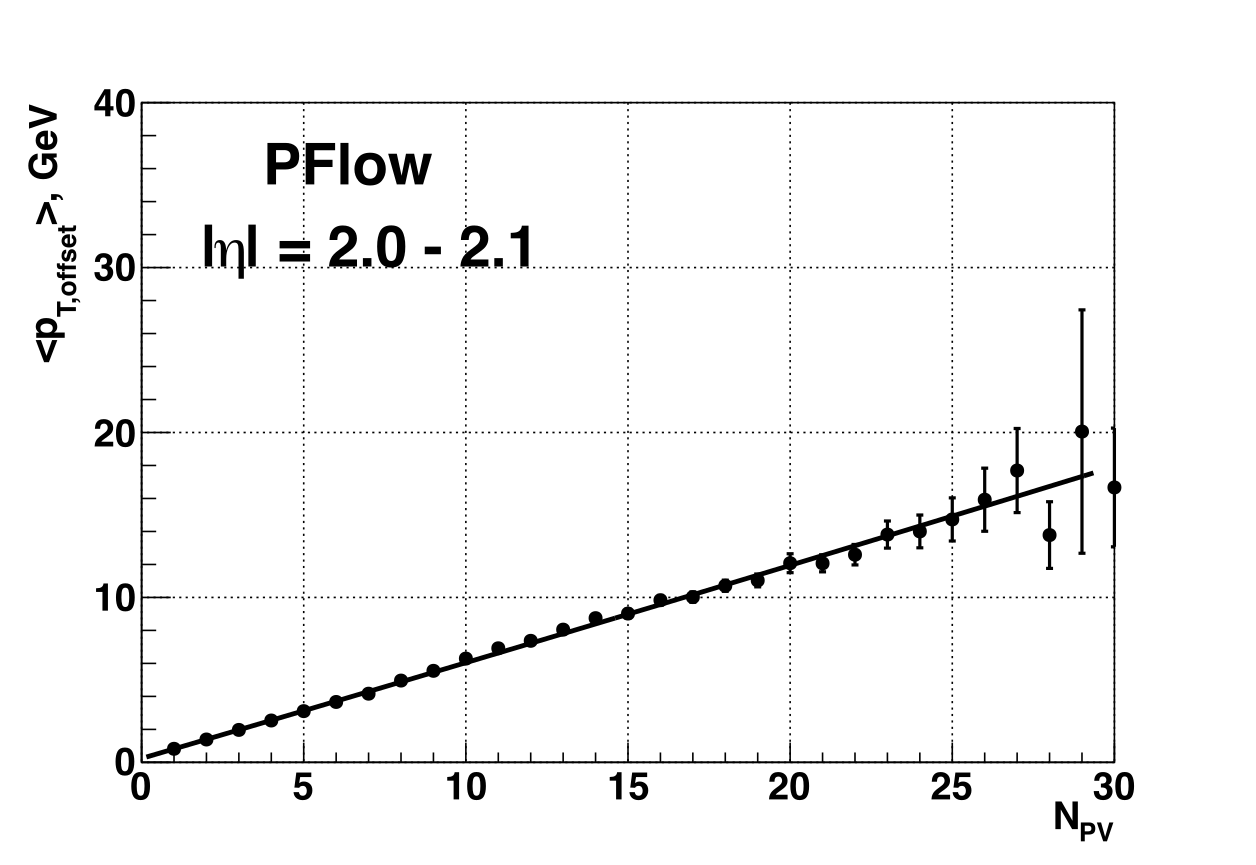
\includegraphics[width=0.45\textwidth]{chapitre4/figs/l1_offset.pdf}} \hfill
  \subcaptionbox{\label{fig:l1_offset_vs_fastjet}}[0.45\textwidth]{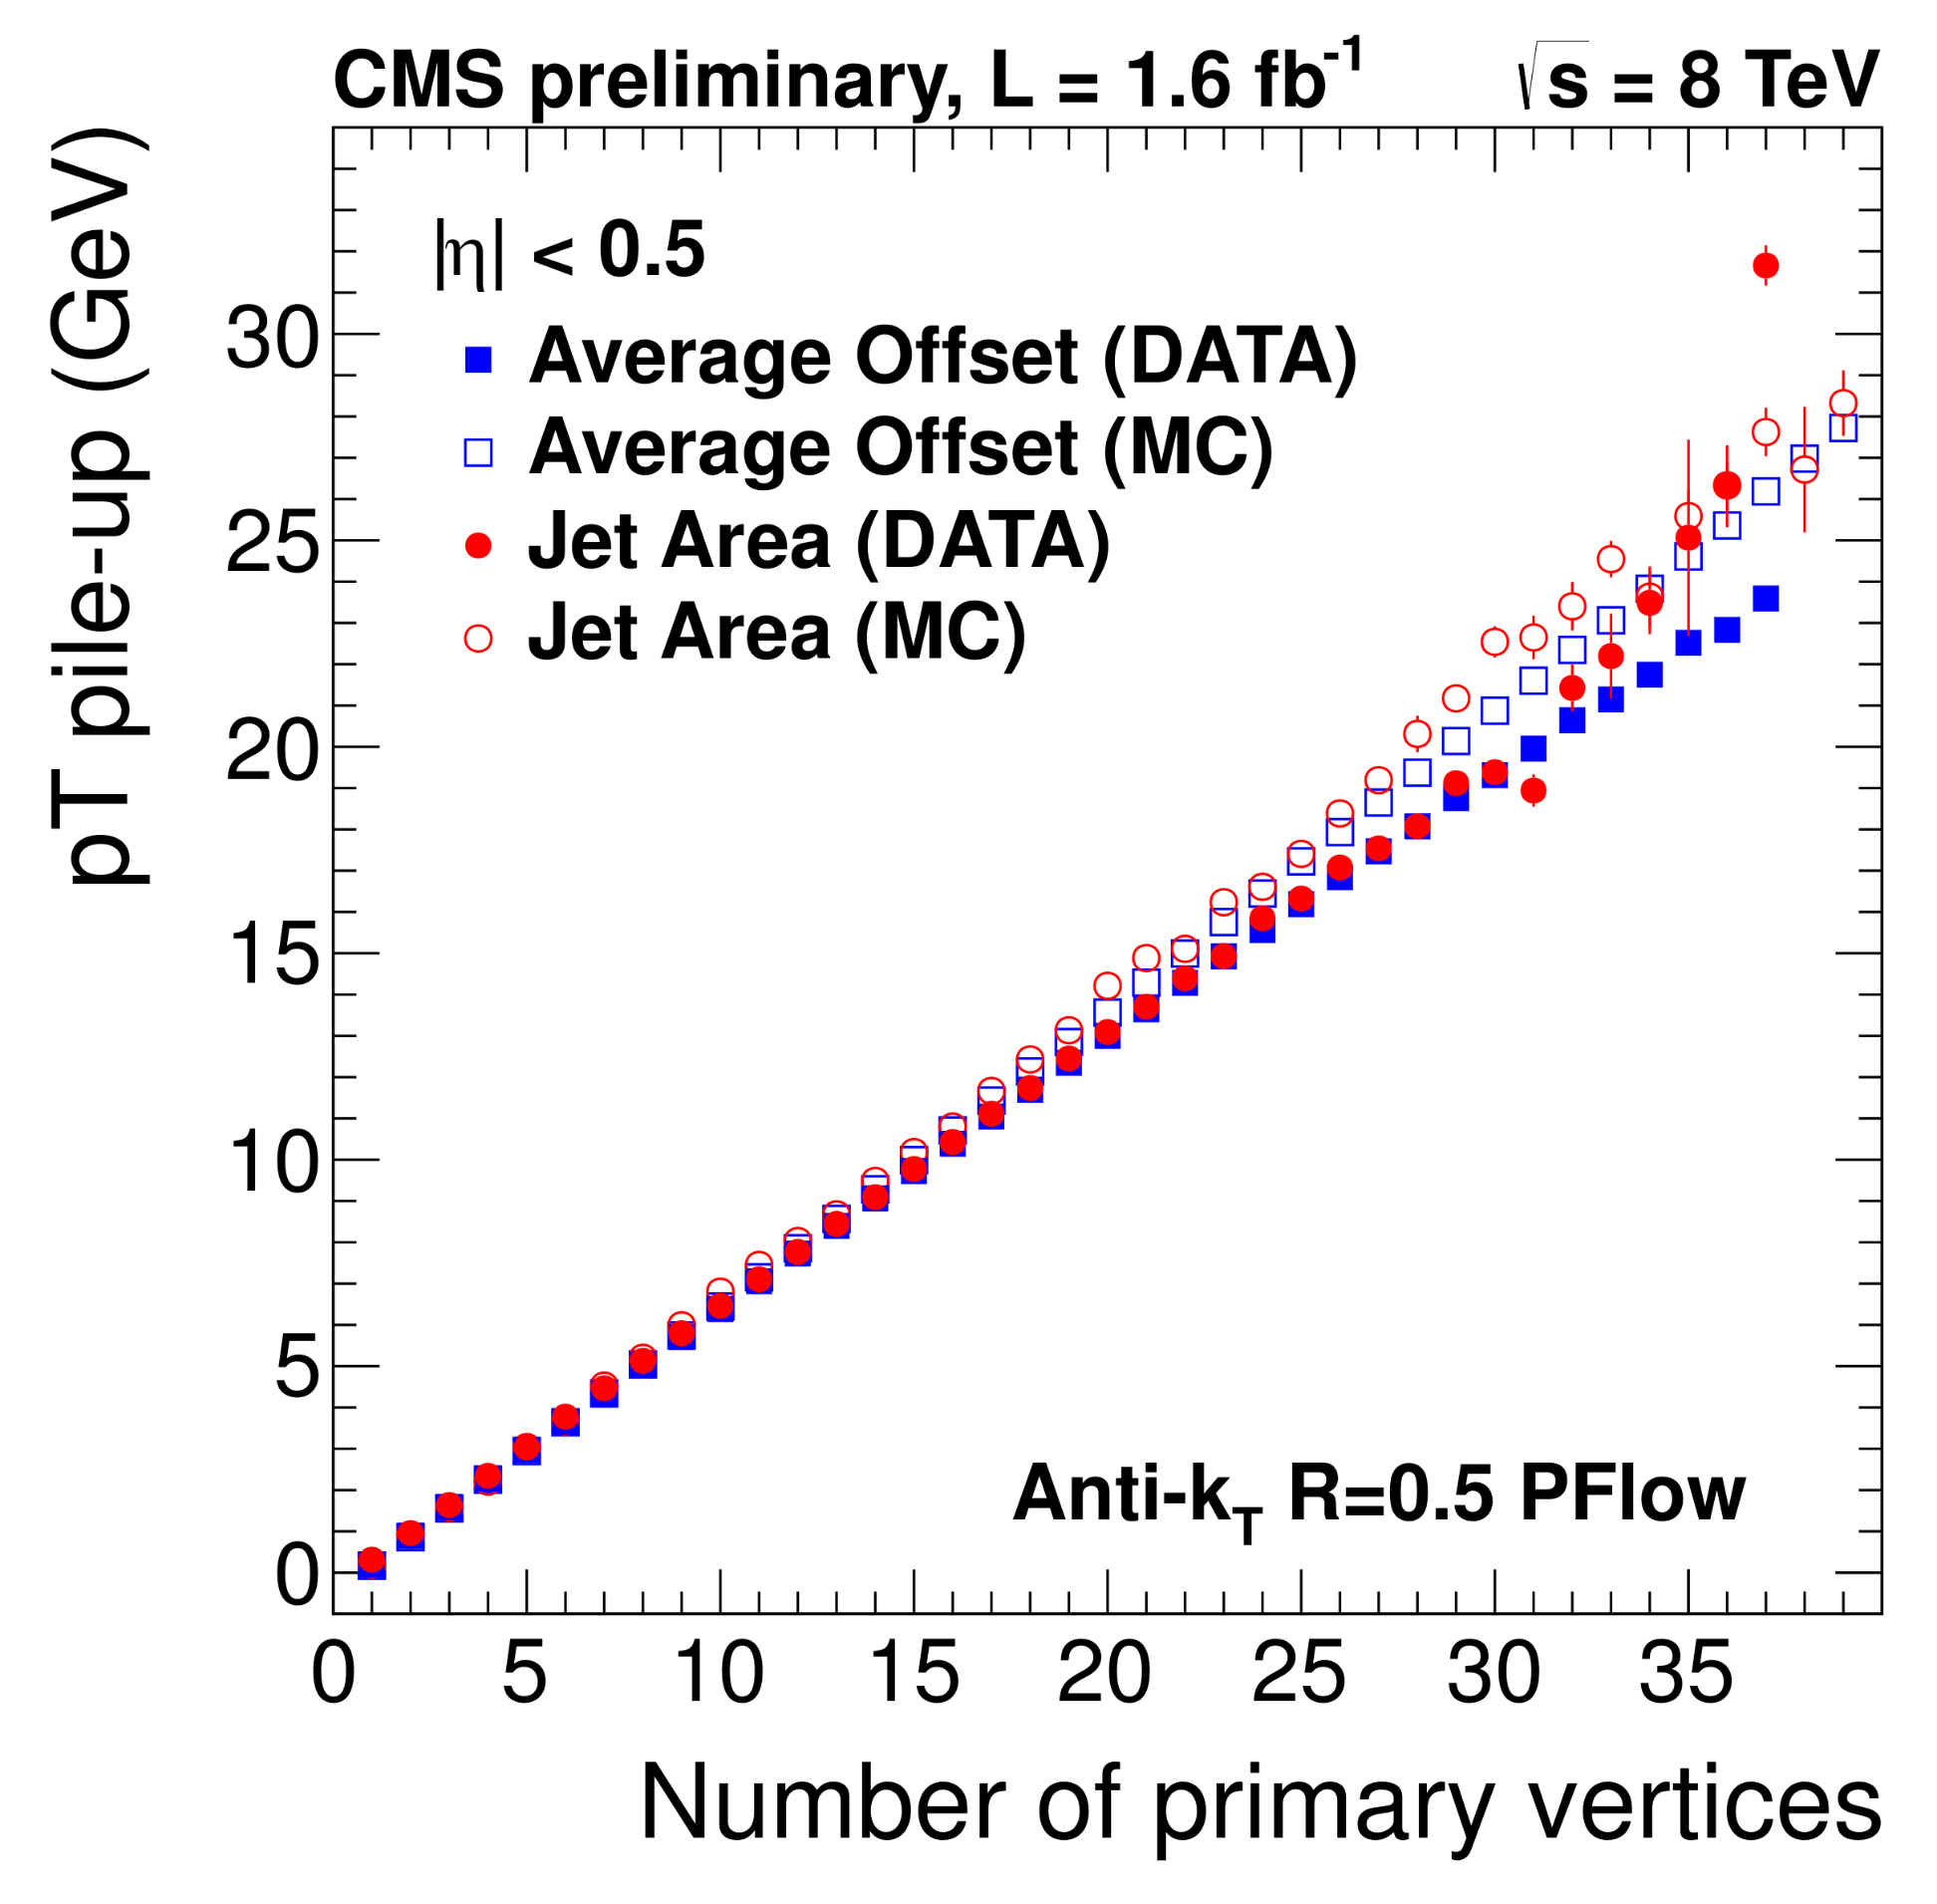
\includegraphics[width=0.45\textwidth]{chapitre4/figs/l1_offset_vs_fastjet.pdf}} \hfill
  \caption{(\subref{fig:l1_offset}) \emph{offset} en fonction du nombre de vertex primaire, pour $\num{2} < \aeta < \num{2.1}$. (\subref{fig:l1_offset_vs_fastjet}) comparaison entre les méthodes \emph{offset} et \emph{fastjet}.}
  \label{fig:jec_l1}
\end{figure}

\subsubsection{La méthode \emph{offset}}

Des événements de biais minimum sont utilisés afin d'estimer l'énergie moyenne portée par un jet à cause du \pu. Cette énergie moyenne est déterminée en fonction du nombre de vertex primaire ($N_{PV}$), une variable directement corrélée au \pu, ainsi qu'en fonction de $\aeta$ (voir \cref{fig:l1_offset}). On obtient ainsi une correction dépendante du nombre de vertex primaires, ainsi que de \aeta. Cette correction est à soustraire de l'énergie du jet afin de supprimer la contribution du \pu.

\subsubsection{La méthode \emph{fastjet}}

Il s'avère que tous les jets ne portent la même énergie due au \pu. La méthode \emph{fastjet} améliore ainsi la méthode \emph{offset} en ajoutant une dépendance des corrections en fonction de l'aire des jets ($A$) et en fonction de la densité d'énergie ($\rho$), définie comme la médiane de la distribution $p_T^j / A_j$, où $j$ est l'index d'un jet dans l'événement. La correction obtenue est donc dépendante de $\rho$, de $A$ et de \aeta. On présente \cref{fig:l1_offset_vs_fastjet} une comparaison entre ces deux méthodes.

\begin{figure}
  \subcaptionbox{\label{fig:l1_no_corr}}[0.45\textwidth]{\includegraphics[width=0.45\textwidth]{chapitre4/figs/l1_effect_no_corr.pdf}} \hfill
  \subcaptionbox{\label{fig:l1_with_corr}}[0.45\textwidth]{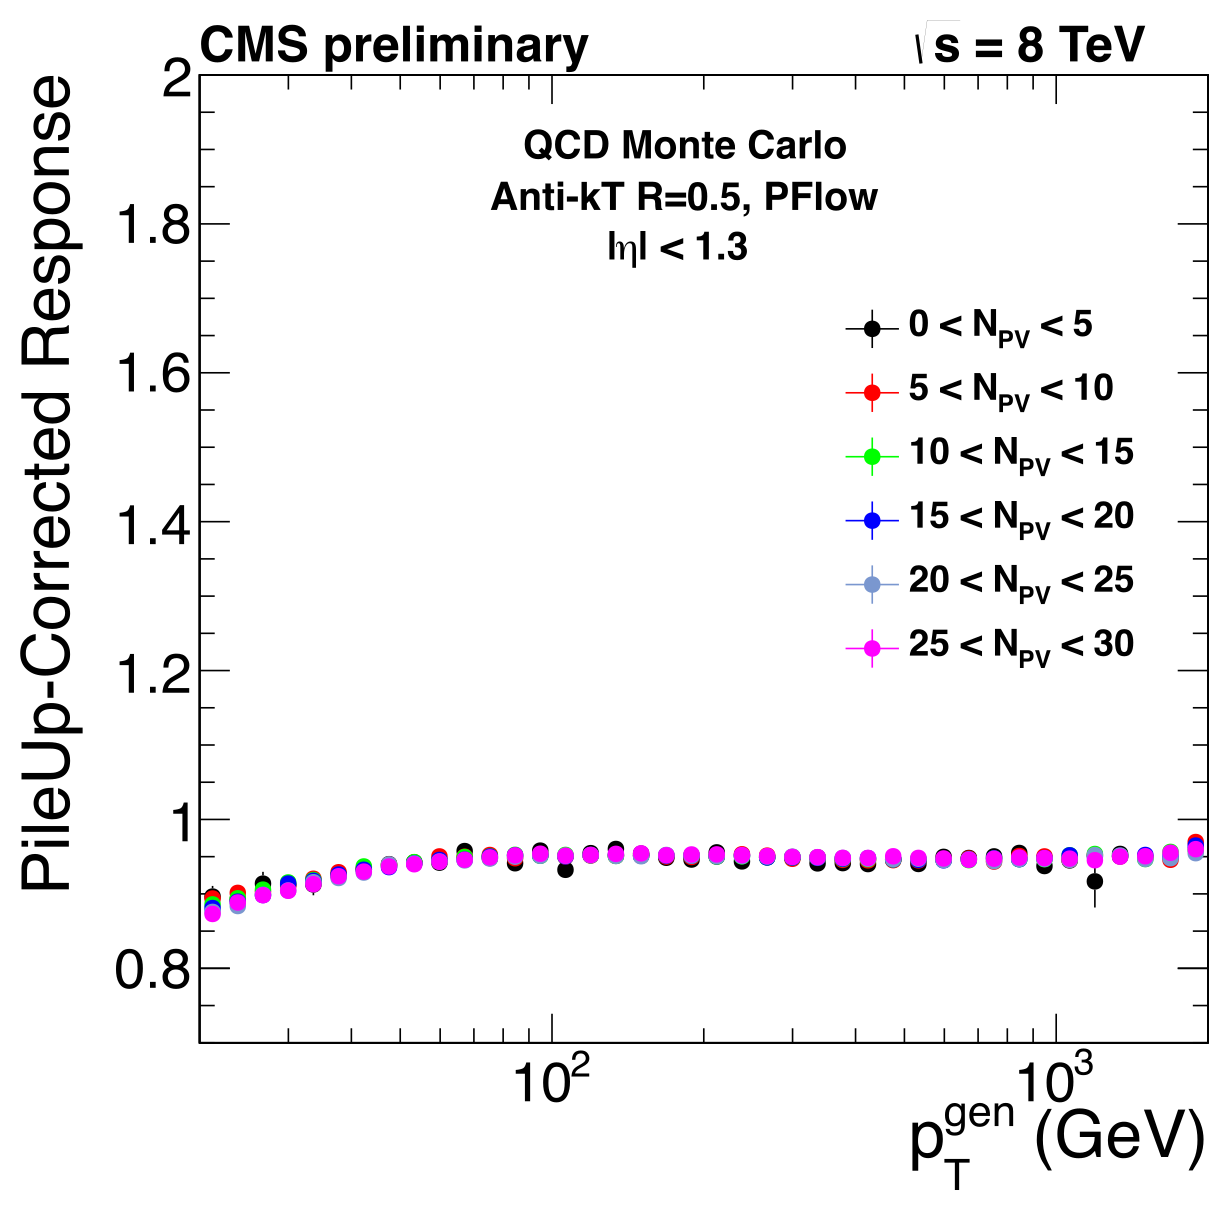
\includegraphics[width=0.45\textwidth]{chapitre4/figs/l1_effect_with_corr.pdf}} \hfill
  \caption{Évolution de la réponse des jets en fonction de l'impulsion transverse simulée, avant l'application des corrections de niveau 1 (\subref{fig:l1_no_corr}) et après (\subref{fig:l1_with_corr}), pour différentes classes de $N_{PV}$.}
  \label{fig:jec_l1_effect}
\end{figure}

\bigskip

Après application des corrections de niveau 1, la réponse des jets, définie comme le rapport en l'impulsion transverse du jet sur l'impulsion transverse vraie, n'est plus dépendante du nombre de vertex primaires, comme on peux le voir \cref{fig:l1_with_corr}.

\subsection{Les corrections de niveau 2 et 3}

Ces corrections sont appliquées après celles de niveau 1. La réponse n'est donc plus dépendante du \pu. Néanmoins, elle varie toujours en fonction de \aeta et du $p_T$. Afin de corriger ces effets, on utilise des événements di-jets. Par conservation de l'impulsion transverse, on a donc $p_T^\text{jet 1} = p_T^\text{jet 2}$. De plus, on considère que les jets dans la région centrale du détecteur ($\aeta < \num{1.3}$) sont correctement reconstruit. On sélectionne donc des événements avec au moins un jet dans la région centrale, et on calcule la réponse $R$, définie comme $p_T^\text{jet} / p_T^\text{central}$, en fonction de \aeta et $p_T$. Dans le cas d'une reconstruction parfaite, la réponse vaut 1. Dans le cas contraire, le facteur de correction à appliquer est $1 / R$.

%\begin{figure}
  %\subcaptionbox{\label{fig:l2l3_response}}[0.45\textwidth]{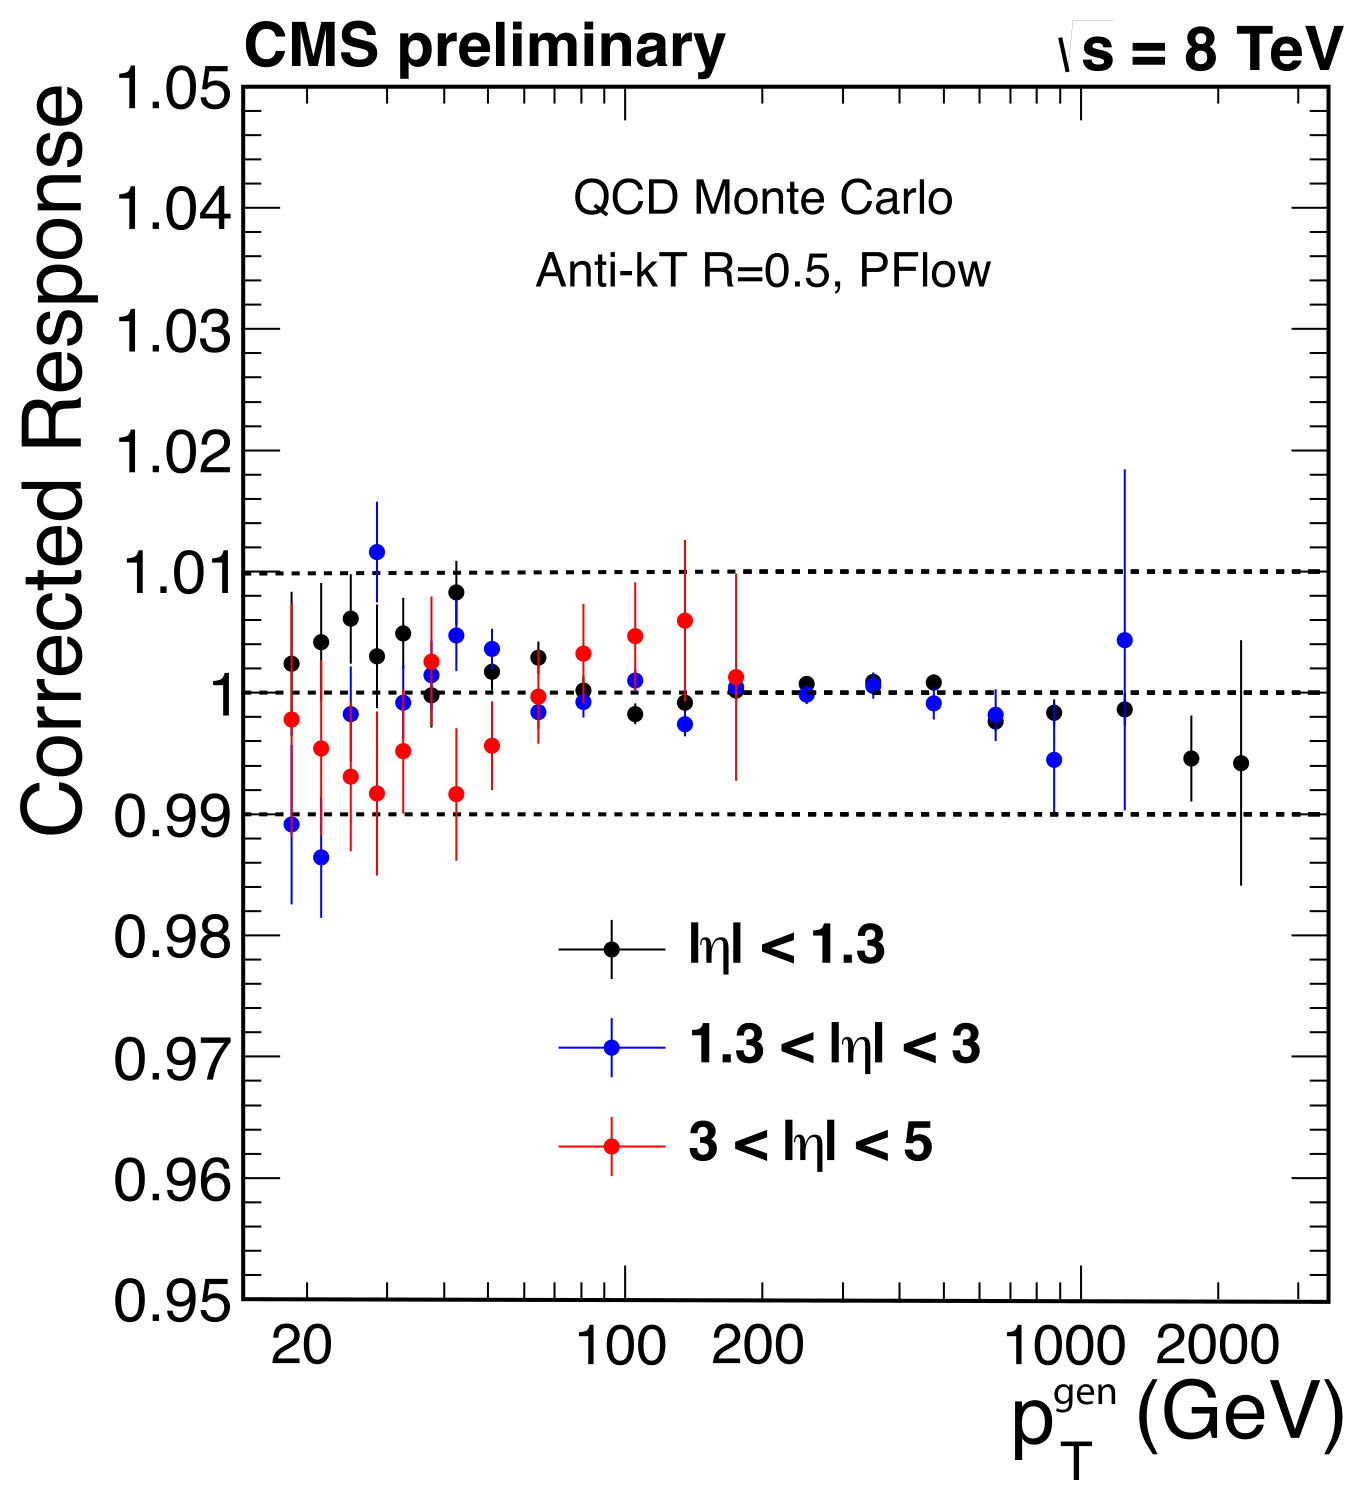
\includegraphics[width=0.45\textwidth]{chapitre4/figs/l2l3_response.pdf}} \hfill
  %\subcaptionbox{\label{fig:l1l2l3}}[0.45\textwidth]{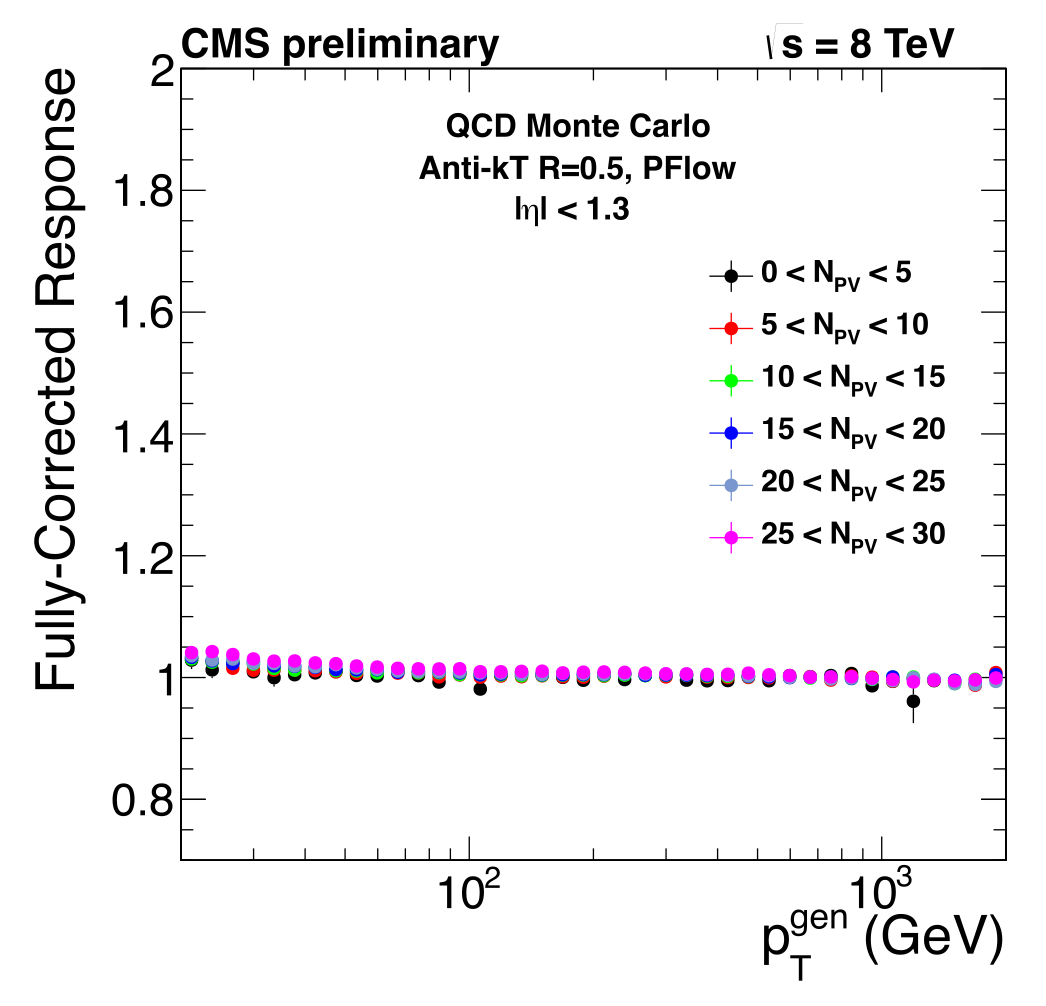
\includegraphics[width=0.45\textwidth]{chapitre4/figs/response_after_l1l2l3.pdf}} \hfill
  %\caption{Évolution de la réponse des jets en fonction de l'impulsion transverse simulée, avant l'application des corrections de niveau 1 (\subref%{fig:l1_no_corr}) et après (\subref{fig:l1_with_corr}), pour différentes classes de $N_{PV}$.}
%  \label{fig:jec_l2l3}
%\end{figure}

\begin{figure}[tbp]
    \centering
    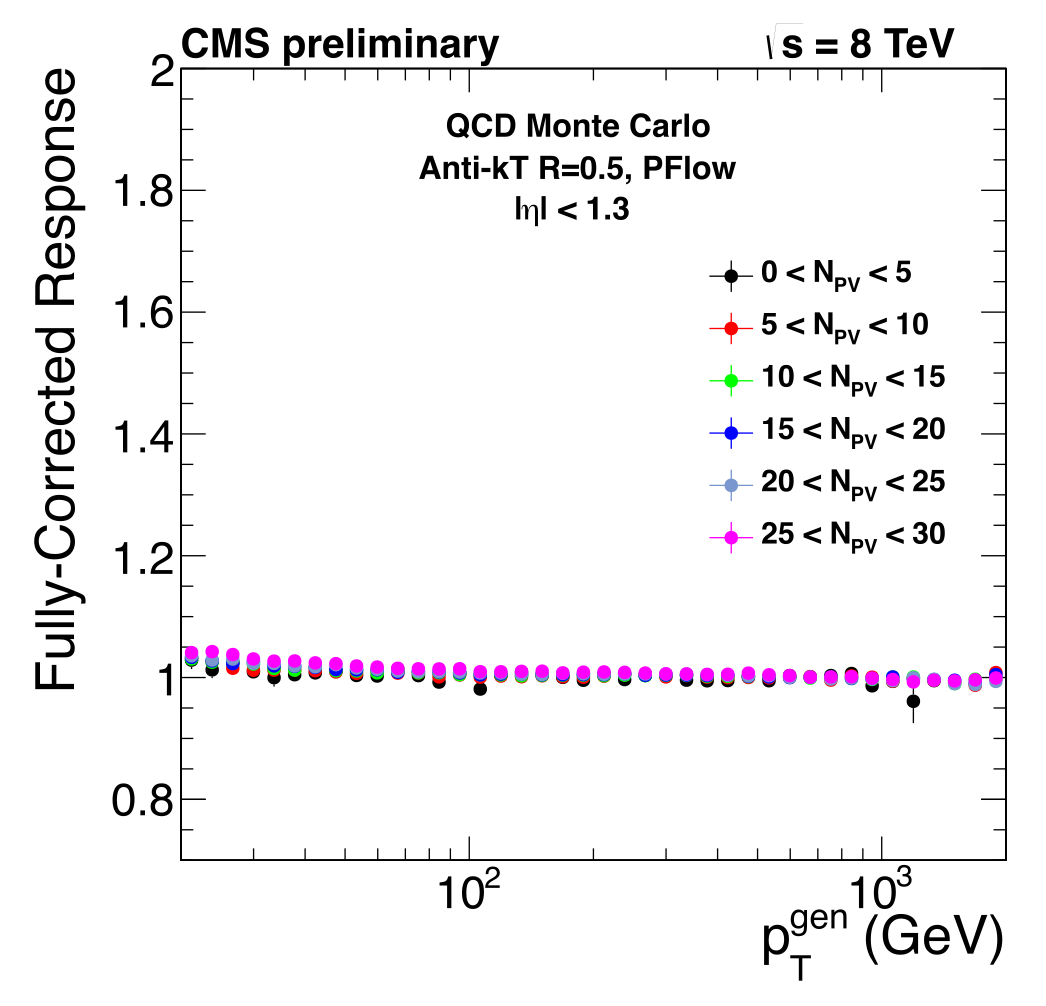
\includegraphics[width=0.55\textwidth]{chapitre4/figs/response_after_l1l2l3.pdf}
    \caption{Réponse des jets après application des corrections de niveau 1, 2 et 3, pour des événements QCD simulés}
    \label{fig:resp_l1l2l3}
\end{figure}

On présente \cref{fig:resp_l1l2l3} la réponse des jets après application des corrections de niveau 1, 2 et 3, pour des événements QCD simulés. La réponse est maintenant linéaire.

\subsection{Les corrections résiduelles}

Les corrections précédentes sont toutes dérivées à l'aide de la simulation. Malheureusement, cette simulation n'est pas parfaite, et des différences existent entre la réponse des jets dans la simulation et dans les données collectées. On applique ainsi un autre niveau de corrections, uniquement sur les données, afin de corriger des dernières différences entre données et simulation. Ces corrections, dépendante de \aeta et du $p_T$ des jets, sont déterminées à l'aide d'événements $\PZ \rightarrow \left[ \Pmuon \APmuon \, | \, \Pelectron \APelectron \right] $ + jets ou $\Pphoton$ + jets, ainsi que des événements di-jets pour la dépendance en \aeta.

Ayant fait l'objet de ma tâche de service au sein de CMS, la détermination des corrections résiduelles à l'aide d'événement $\Pphoton$ + jets est décrite en détails dans la \cref{sec:jetmet_gamma_jet}.

\subsection{Erreurs systématiques}

\begin{figure}[tbp]
    \centering
    \subcaptionbox{\label{fig:uncertainties_vs_pt}}[0.45\textwidth]{\includegraphics[width=0.45\textwidth]{chapitre4/figs/uncertainties/uncertainties_vs_pt.pdf}} \qquad
    \subcaptionbox{\label{fig:uncertainties_vs_eta}}[0.45\textwidth]{\includegraphics[width=0.45\textwidth]{chapitre4/figs/uncertainties/uncertainties_vs_eta.pdf}}
    \caption{Erreurs systématiques associées aux corrections des jets en fonction de \pt (\subref{fig:uncertainties_vs_pt}) pour $\aeta \simeq 0$, et en fonction de \aeta (\subref{fig:uncertainties_vs_eta}) pour $\pt = \SI{100}{\GeV}$.}
    \label{fig:jetmet_uncertainties}
\end{figure}

Face à la complexité de la détermination des corrections des jets, l'erreur systématique associée est souvent l'erreur dominante dans les analyses de physique, atteignant souvent des valeurs proches de \SI{10}{\%}. Beaucoup d'efforts sont fait pour améliorer notre compréhension des détecteurs et ainsi réduire ces erreurs systématiques.

\medskip

On trouve \cref{fig:jetmet_uncertainties} l'évolution des erreurs systématiques en fonction de \pt (\cref{fig:uncertainties_vs_pt}) et en fonction de \aeta (\cref{fig:uncertainties_vs_eta}). Cette erreur se décompose en 6 sources indépendantes, et on constate que la présence de \pu (ligne bleue) contribue en majorité à l'incertitude totale. De nouvelles techniques de suppression du \pu au niveau 1 sont ainsi en cours de développement, afin de réduire cette erreur systématique. Néanmoins, pour des jets de \SI{100}{\GeV} dans le tonneau ($\aeta < \num{1.3}$), on arrive à garder l'erreur systématique totale sous la barre des \SI{2}{\%}.

\section{Détermination des corrections résiduelles à l'aide d'événements \texorpdfstring{$\Pphoton$}{γ} + jets} \label{sec:jetmet_gamma_jet}

\subsection{Intérêt des événements \texorpdfstring{$\Pphoton$}{γ} + jets}

On cherche à corriger des dernières différences entre simulation et données collectées. Pour cela, on mesure la réponse des jets dans les données, ainsi que dans la simulation, et on corrige les données pour coller à la simulation. Il est donc nécessaire d'utiliser un processus physique qui permet de connaître de façon la plus précise possible l'énergie d'un jet, sans avoir à utiliser la vérité de la simulation.

\begin{figure}[t!] \centering
  \subcaptionbox{\label{fig:g_plus_jet_1}}[.4\linewidth]{
  \begin{fmfgraph*}(180,120)
    \fmfpen{0.5}
    \fmfleft{i1,i2}
    \fmfright{o1,o2}
    \fmf{gluon}{i1,v1}
    \fmf{fermion}{i2,v1}
    \fmf{fermion,label=\Pquark}{v1,v2}
    \fmf{fermion}{v2,o1}
    \fmf{photon}{v2,o2}
    \fmffreeze
    \fmfdot{v1,v2}
    \fmflabel{\Pquark}{i2}
    \fmflabel{\Pquark}{o1}
    \fmflabel{\Pphoton}{o2}
  \end{fmfgraph*}}\qquad \quad%
  % \begin{fmfgraph*}(180,120)
  %   \fmfpen{0.5}
  %   \fmfleft{i1,i2}
  %   \fmfright{o1,o2,o3}
  %   \fmf{gluon}{i2,v1}
  %   \fmf{gluon}{v3,o1}
  %   \fmf{fermion}{i1,v3}
  %   \fmf{fermion,label=\APquark}{v3,v2,v1}
  %   \fmf{fermion}{v1,o3}
  %   \fmffreeze
  %   \fmf{photon,label=\Pphoton}{v2,o2}
  %   \fmfdot{v1,v2,v3}
  %   \fmflabel{\Pquark}{i1}
  %   \fmflabel{\Pquark}{o3}
  % \end{fmfgraph*}}\qquad \quad%
  \subcaptionbox{\label{fig:g_plus_jet_2}}[.4\linewidth]{
  \begin{fmfgraph*}(180,120)
    \fmfpen{0.5}
    \fmfstraight
    \fmfleft{i1,i2}
    \fmfright{o1,o2,o3}
    \fmf{fermion}{i1,v1,i2}
    \fmf{fermion}{v4,v2}
    \fmf{phantom}{o1,v4}
    \fmf{fermion,label=\Pquark}{v2,v3}
    \fmf{photon,label=$\Pphoton$}{v3,o3}
    \fmf{gluon}{v1,v2}
    \fmffreeze
    \fmf{fermion}{v3,o2}
    \fmfdot{v1,v2,v3}
    \fmflabel{\APquark}{i2}
    \fmflabel{\Pquark}{i1}
    \fmflabel{\Pquark}{o2}
    \fmflabel{\APquark}{v4}
  \end{fmfgraph*}
  }
  \caption{Diagrammes de Feynman associés à la production d'un photon et d'un jet (\subref{fig:g_plus_jet_1}) et d'un photon et de deux jets (\subref{fig:g_plus_jet_2}).}
  \label{fig:gamma_jet_diagrams}
\end{figure}

On utilise pour cela des processus comportant uniquement deux particules dans l'état final : une particule dont on connaît très bien les propriétés (boson \PZ, photon, \ldots), qui sera notre sonde, et un jet. On utilise ensuite les propriétés de la sonde pour déterminer celles du jet. Par la suite, seul les événements \Pphoton + jets seront abordés.

\bigskip

On présente \cref{fig:gamma_jet_diagrams} deux diagrammes de Feynman représentant la production d'un photon accompagné d'un ou deux jets. L'impulsion dans le plan transverse étant nulle au moment de la collision, on a dans l'état final
\begin{align*}
  \vec{p}_T &= 0 = \vec{p}_{T}^{\Pphoton} + \vec{p}_T^\text{jet}\\
  \norm{\vec{p}_T^{\Pphoton}} &= \norm{\vec{p}_T^{\text{jet}}}
\end{align*}

Ainsi, il est suffisant de connaître l'impulsion transverse de la sonde pour déterminer l'impulsion transverse du jet. Le calorimètre électromagnétique étant bien plus performant que le calorimètre hadronique, on voit ici tout l'intérêt du choix du photon comme sonde.

\subsection{Détermination de la réponse des jets}

On cherche à déterminer la réponse $R$ des jets, qui tend vers 1 si l'on reconstruit parfaitement le jet. On utilise deux méthodes différentes pour déterminer cette réponse : la méthode de la balance et la méthode MPF, détaillées ci-dessous.

\subsubsection{La méthode de la balance}

On utilise le principe de conservation de l'impulsion transverse. On a alors
\begin{align*}
  \norm{\vec{p}_T^{\Pphoton}} &= \norm{\vec{p}_T^{jet}}
\end{align*}
et on défini la réponse $R$ par la relation
\begin{align*}
    R &= \frac{p_T^\text{jet}}{p_T^{\Pphoton}}
\end{align*}

Cette méthode est très simple et performante. Néanmoins, elle est très sensible au \pu, ainsi qu'aux radiations dans l'état final. En effet, la présence d'autres jets dans l'état final vont venir perturber la balance entre le jet et le photon. On verra par la suite comment restaurer cette balance.

\subsubsection{La méthode MPF (\emph{Missing $E_T$ projection fraction})}

Un événement \Pphoton + jets n'a pas de \met. Ainsi, au niveau partonique, on a
\begin{align*}
  \vec{p}_T^{\Pphoton} + \vec{p}_T^{\text{recul}} &= -\vec{\met} = \vec{0}
\end{align*}
où $\vec{p}_T^{\text{recul}}$ est le vecteur impulsion transverse de toutes les particules dans l'événement différentes du photon.

Après reconstruction, on a
\begin{align*}
  R_{\Pphoton} \, \vec{p}_T^{\Pphoton} + R_{\text{recul}} \, \vec{p}_T^{\text{recul}} &= -\vec{\met}
\end{align*}
$R_X$ désigne ici la réponse des détecteurs lors de la reconstruction de l'objet $X$.

On considère que les photons sont reconstruits de façon parfaite, on pose donc $R_{\Pphoton} = 1$. En utilisant le fait que $\vec{p}_T^{\text{recul}} = -\vec{p}_T^{\Pphoton}$ on obtient
\begin{align*}
  R_{\text{recul}} &= 1 + \frac{\vec{\met} \cdot \vec{p}_T^{\Pphoton}}{\left( p_T^{\Pphoton} \right)^2} \equiv R_{\text{MPF}}
\end{align*}

Cette méthode n'est pas dépendante de la présence de jets additionnels dans l'événement, mais requiert par contre une excellente reconstruction de l'énergie transverse manquante. C'est le cas dans CMS grâce à l'utilisation de l'algorithme du \pf.

\medskip

Cette méthode est utilisée pour produire les corrections officielles. La méthode de la balance permet de vérifier la compatibilité des corrections obtenues.

\subsubsection{L'extrapolation}

La balance entre le photon et le jet est perturbée par la présence de jets additionnels dans l'événement, provenant soit du \pu, soit de radiations dans l'état final. On définit $\alpha$ comme le rapport entre l'impulsion transverse du second jet de l'événement et l'impulsion transverse du photon,
\begin{align*}
    \alpha &= \frac{p_T^{\text{\ordinalnum{2} jet}}}{p_T^\gamma}
\end{align*}

Afin de réduire l'influence des jets additionnels sur la réponse, on effectue un découpage de la réponse en $\alpha$, et on extrapole le comportement de la réponse pour $\alpha \rightarrow 0$. On verra plus loin que cette extrapolation est efficace pour la réponse obtenue avec la méthode de la balance, et inutile pour la méthode MPF.

\end{fmffile}

\subsection{Sélection des événements}

On cherche à sélectionner des événements contenant un unique photon, ainsi qu'un ou deux jets. Le principal bruit de fond est dû aux événements multi-jets (de type $\Pquark \APquark \rightarrow \Pquark \APquark$) où un jet est identifié incorrectement comme un photon. On utilise comme signal des événements $\Pphoton$ + jets simulés.

Afin d'éliminer une grande partie du bruit du fond, une sélection est appliquée. La première étape consiste à sélectionner des événements contenant uniquement un seul photon. On utilise pour cela une méthode d'identification des photons, qui permet selon les analyses d'obtenir une grande efficacité ou une grande pureté. On choisit le point de fonctionnement qui offre la plus grande pureté ($\tilde \SI{96}{\%}$), au détriment de l'efficacité ($\tilde \SI{70}{\%}$). Cette identification est définie de la façon suivante :

\begin{enumerate}
    \item Un contrôle est effectué pour vérifier que le photon n'est pas en réalité un électron, et qu'il ne provient pas de la conversion d'un électron lors de son passage dans le ECAL.
    \item Le ratio entre l'énergie collectée dans le calorimètre hadronique et l'énergie collectée dans le calorimètre électromagnétique doit être inférieur à \SI{5}{\%}. La majorité de l'énergie doit donc être déposée dans le calorimètre électromagnétique.
    \item $\sigma_{i\eta i\eta} < \num{0.011}$. Cette variable représente la largeur de l'agrégat calorimétrique en \aeta, et est caractéristique de la forme de la gerbe électronique dans le calorimètre électromagnétique, plus étalée dans le cas d'un électron que d'un photon. \fxnote{Définition ? Voir \url{https://indico.cern.ch/event/27560/material/slides/1?contribId=1}}
\end{enumerate}

En plus de ces trois critères, on demande à ce que le photon soit isolé. On définit l'isolation $I$ comme le rapport entre l'énergie de toutes les particules \pf contenues dans un cône de rayon $\Delta R = \num{0.3}$ centré autour du photon et l'énergie du photon. Cette valeur étant hautement sensible au \pu, on applique une procédure qui permet de diminuer son impact, en corrigeant cette isolation par un facteur dépendant de la densité d'énergie $\rho$. On a ainsi $I_\text{corr} = \max{\left(I - f(\rho), 0\right)}$. On effectue des coupures sur cette isolation selon trois différents types de particules : les hadrons neutres, chargés, et les photons :

\begin{itemize}
    \item $I_\text{hadrons neutres} < \num{0.4} + \num{0.04} \, p_T^{\Pphoton}$
    \item $I_\text{hadrons chargés} < \num{0.7}$
    \item $I_\text{photons} < \num{0.5} + \num{0.005} \, p_T^{\Pphoton}$
\end{itemize}

Afin de ne garder que les photons les mieux reconstruits, on sélectionne uniquement ceux reconstruits dans le tonneau, avec $\aeta < \num{1.3}$, et une impulsion transverse d'au moins \SI{40}{\GeV}.

\medskip

On demande en plus au moins un bon jet dans l'événement, reconstruit grâce à l'algorithme anti-$k_T$, avec une largeur $R = \num{0.5}$. Cette identification est très efficace ($> \SI{99}{\%}$) et permet d'éliminer les faux jets dû à des bruits dans les détecteurs. La séparation azimutale $\abs{\Delta \phi}$ dans le plan transverse entre le photon et le premier jet de l'événement doit être supérieure à \SI{2.8}{\radian}, afin de ne conserver que les événements où le photon et le jet sont dos-à-dos. Les \cref{fig:schema_gamma_jet,fig:schema_gamma_jets} représentent un événement $\Pphoton$ + jets avec 1 ou 2 jets. Dans le cas où un second jet est présent, on vérifie que son énergie est inférieure à \SI{20}{\%} de celle du photon ($\alpha < \num{0.20}$), afin d'éviter de conserver des événements trop déséquilibrés. Cette condition n'est appliquée que si $p_T^{\text{\ordinalnum{2} jet}} \geq \SI{10}{\GeV}$. Tous les jets sont corrigés avec les corrections de niveau 1, 2 et 3. Cependant, les corrections résiduelles ne sont pas appliquées sur les données puisque ce sont ces corrections que l'on souhaite déterminer au travers de cette analyse. Toutes les corrections effectuées sur les jets sont ensuite propagées à l'énergie transverse manquante.

\begin{figure}[tbp] \centering
  \subcaptionbox{\label{fig:schema_gamma_jet}}[0.45\textwidth]{\scalebox{2}{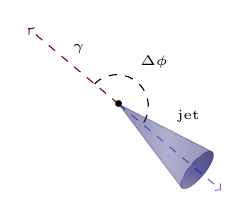
\begin{tikzpicture}[rotate=45]
    \draw[draw=red!50!black,dashed,->] (0:0) -- (95:1.5) ;
    \draw (90:1) node[right] {\tiny $\gamma$} ;

    \draw[draw=blue!60,dashed,->] (0:0) -- (-85:1.7) ;

    \draw[dashed] (95:4mm) arc (90:-80:4mm) ;
    \draw (5:7mm) node {\tiny $\Delta\phi$} ;

    \begin{scope}[rotate=5]
      \fill[top color=blue!50!black,bottom color=blue!10,middle color=blue,shading=axis,opacity=0.25] (0,-13mm) circle (3mm and 1mm);
      \fill[left color=blue!50!black,right color=blue!50!black,middle color=blue!50,shading=axis,opacity=0.25] (3mm,-13mm) -- (0,0mm) -- (-3mm,-13mm) arc (180:360:3mm and 1mm);
      \draw[draw=blue!50!black,opacity=0.25] (-3mm,-13mm) arc (180:360:3mm and 1mm) -- (0,0mm) -- cycle;
      \draw[draw=blue!50!black,opacity=0.25,densely dashed] (-3mm,-13mm) arc (180:0:3mm and 1mm);
    \end{scope}

    \draw (-55:0.9) node {\tiny jet} ;
    \draw (0:0) node {\tiny $\bullet$} ;

  \end{tikzpicture}}} \quad
  \subcaptionbox{\label{fig:schema_gamma_jets}}[0.45\textwidth]{\scalebox{2}{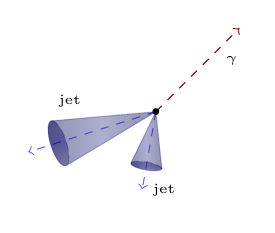
\begin{tikzpicture}
    \draw[draw=red!50!black,dashed,->] (0:0) -- (45:1.5) ;
    \draw (40:1) node[right] {\tiny $\gamma$} ;

    \draw[draw=blue!60,dashed,->] (0:0) -- (-100:1) ;
    \draw[draw=blue!60,dashed,->] (0:0) -- (-162.5:1.7) ;

    \begin{scope}[rotate=-72]
      \fill[top color=blue!50!black,bottom color=blue!10,middle color=blue,shading=axis,opacity=0.25] (0,-13mm) circle (3mm and 1mm);
      \fill[left color=blue!50!black,right color=blue!50!black,middle color=blue!50,shading=axis,opacity=0.25] (3mm,-13mm) -- (0,0mm) -- (-3mm,-13mm) arc (180:360:3mm and 1mm);
      \draw[draw=blue!50!black,opacity=0.25] (-3mm,-13mm) arc (180:360:3mm and 1mm) -- (0,0mm) -- cycle;
      \draw[draw=blue!50!black,opacity=0.25,densely dashed] (-3mm,-13mm) arc (180:0:3mm and 1mm);
    \end{scope}

    \begin{scope}[rotate=-10]
      \fill[top color=blue!50!black,bottom color=blue!10,middle color=blue,shading=axis,opacity=0.25] (0,-7mm) circle (2mm and 0.5mm);
      \fill[left color=blue!50!black,right color=blue!50!black,middle color=blue!50,shading=axis,opacity=0.25] (2mm,-7mm) -- (0,0mm) -- (-2mm,-7mm) arc (180:360:2mm and 0.5mm);
      \draw[draw=blue!50!black,opacity=0.25] (-2mm,-7mm) arc (180:360:2mm and 0.5mm) -- (0,0mm) -- cycle;
      \draw[draw=blue!50!black,opacity=0.25,densely dashed] (-2mm,-7mm) arc (180:0:2mm and 0.5mm);
    \end{scope}

    \draw (-84:1) node {\tiny jet} ;
    \draw (-187:1.1) node {\tiny jet} ;
    \draw (0:0) node {\tiny $\bullet$} ;

  \end{tikzpicture}}}
  \caption{Un événement $\gamma$ + jets parfaitement dos-à-dos (\subref{fig:schema_gamma_jet}) et où la balance est brisée (\subref{fig:schema_gamma_jets}).}
  \label{fig:schema_g_jet}
\end{figure}

Pour terminer la sélection, un véto est imposé sur la présence d'électrons ou de muons dans l'événement. Sur des événements de signal simulés, cette sélection a une efficacité de \tilde \SI{20}{\%}, et inférieure à \tilde\SI{1}{‰} sur le bruit de fond. On présente \cref{fig:pt_photon_jet} une comparaison entre la simulation et les données pour l'impulsion transverse du photon, du premier jet de l'événement, du second, ainsi que l'énergie transverse manquante. L'incertitude sur la simulation comprend l'incertitude statistique, l'incertitude sur la luminosité de \SI{2.6}{\%}, ainsi qu'une incertitude de \SI{10}{\%} comprenant l'incertitude sur l'estimation de la section efficace \Pphoton + jets et multi-jets.

\begin{figure}[p]
    \centering
    \subcaptionbox{\label{pt_photon}}[0.45\textwidth]{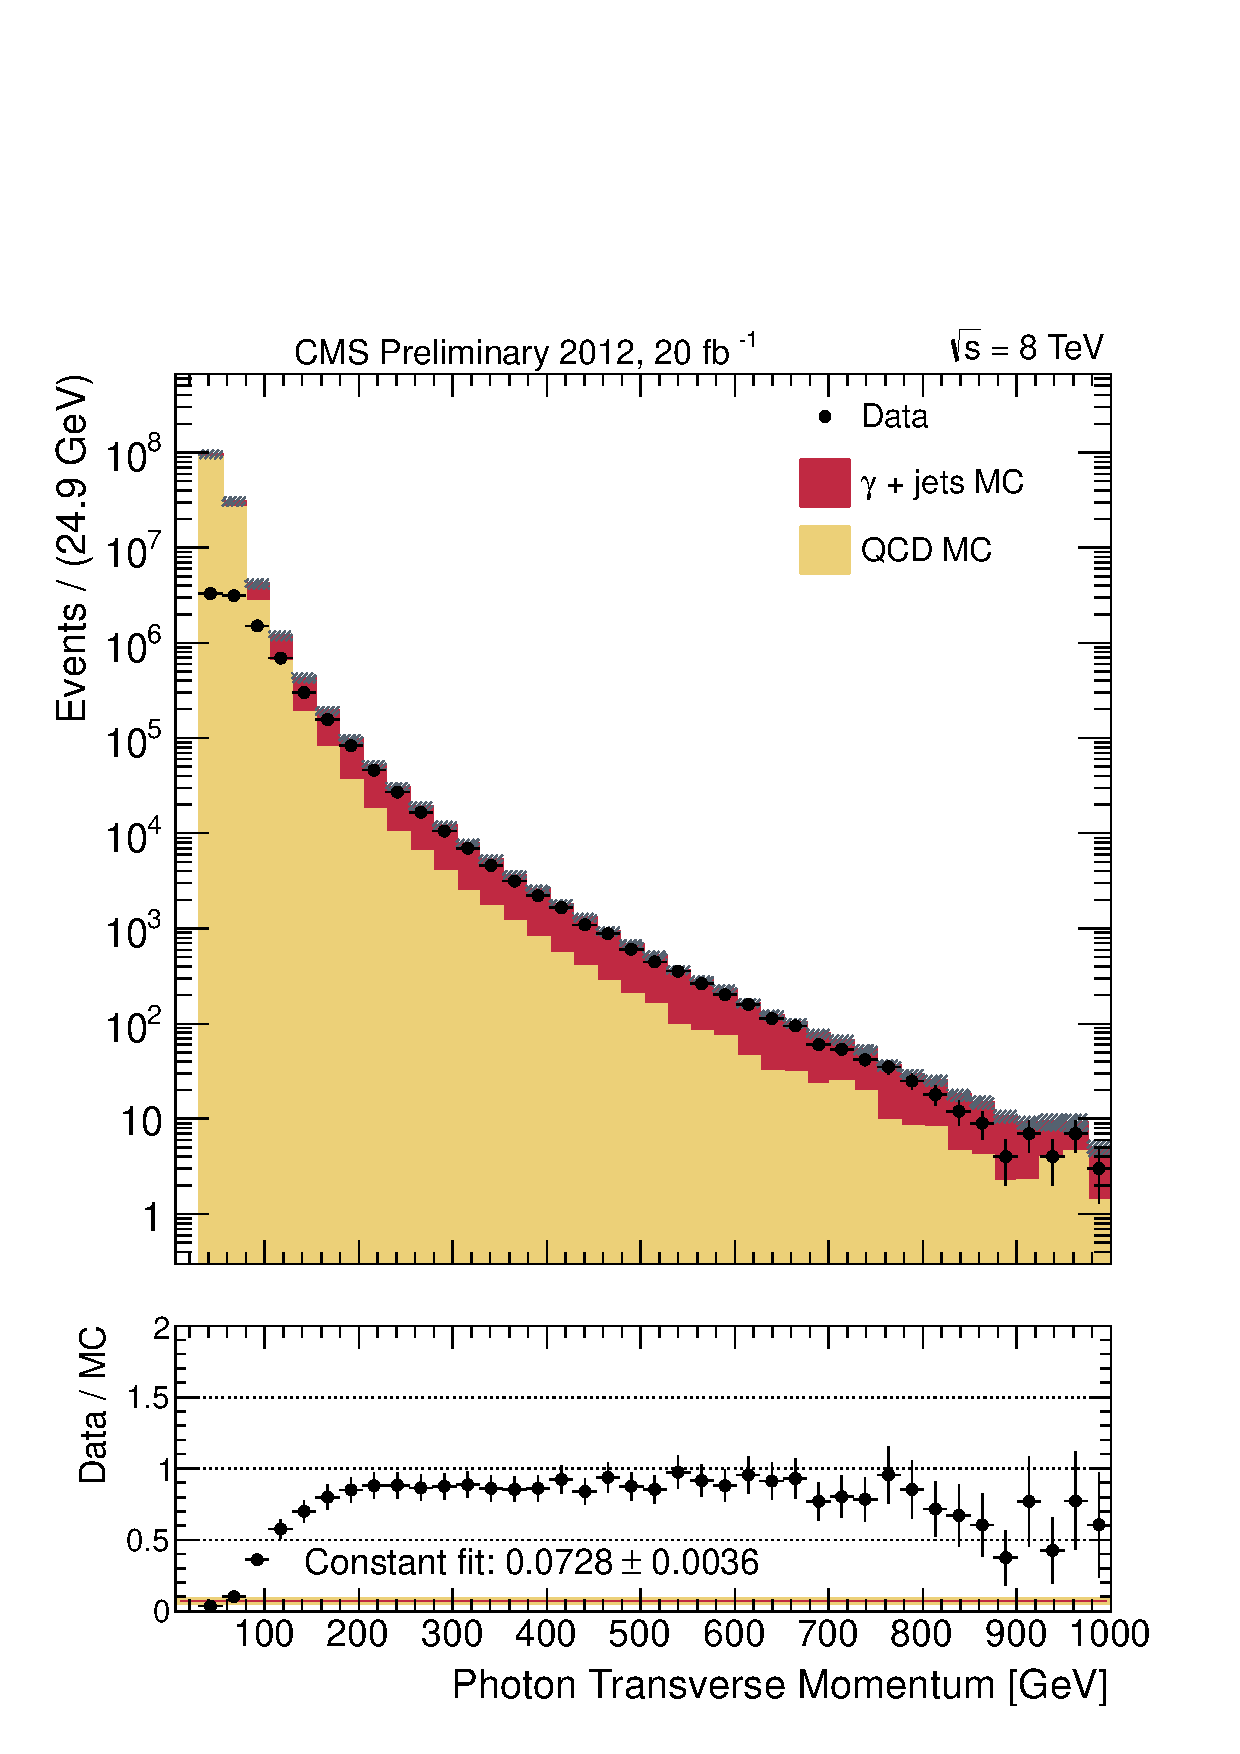
\includegraphics[width=0.45\textwidth]{chapitre4/figs/ptPhoton_passedID_log.pdf}}\hfill
    \subcaptionbox{\label{pt_first_jet}}[0.45\textwidth]{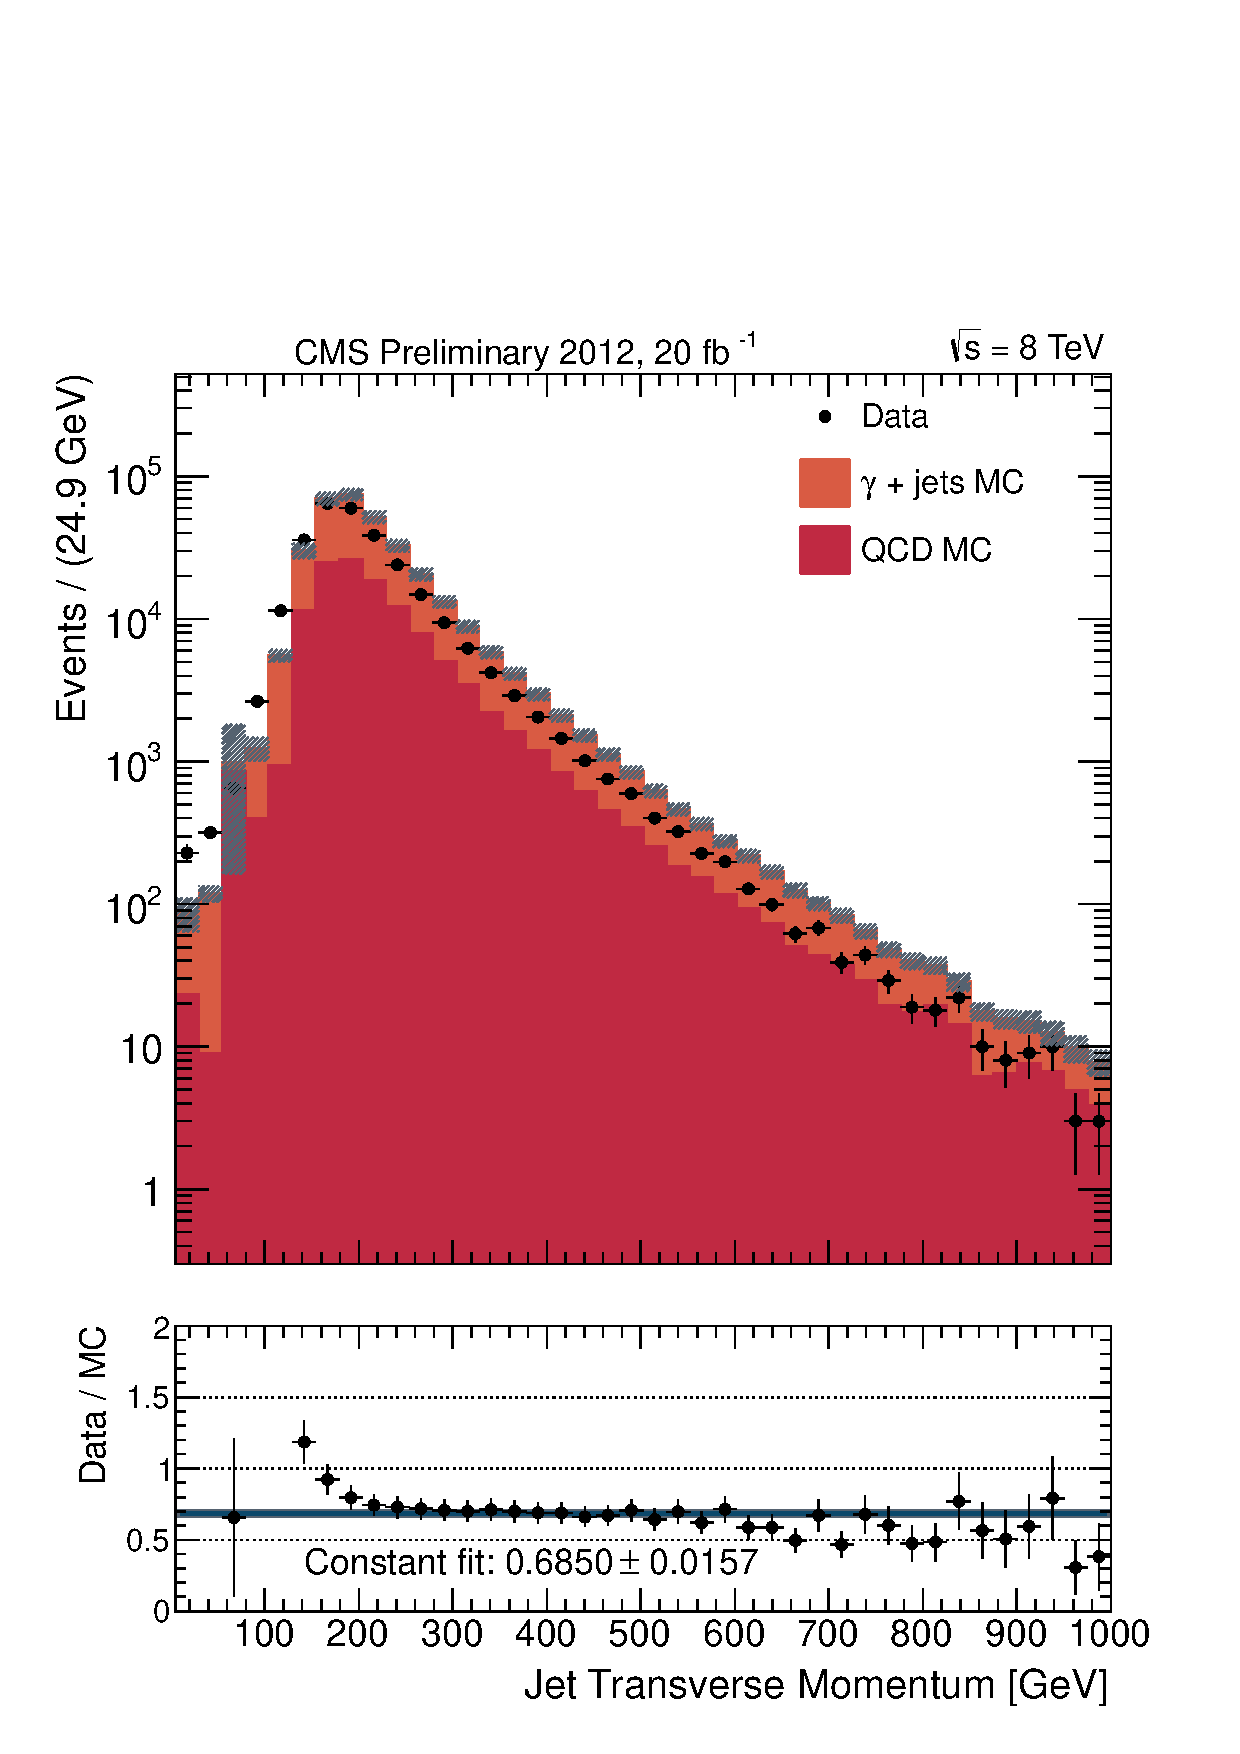
\includegraphics[width=0.45\textwidth]{chapitre4/figs/ptFirstJet_passedID_log.pdf}}
    \subcaptionbox{\label{pt_second_jet}}[0.45\textwidth]{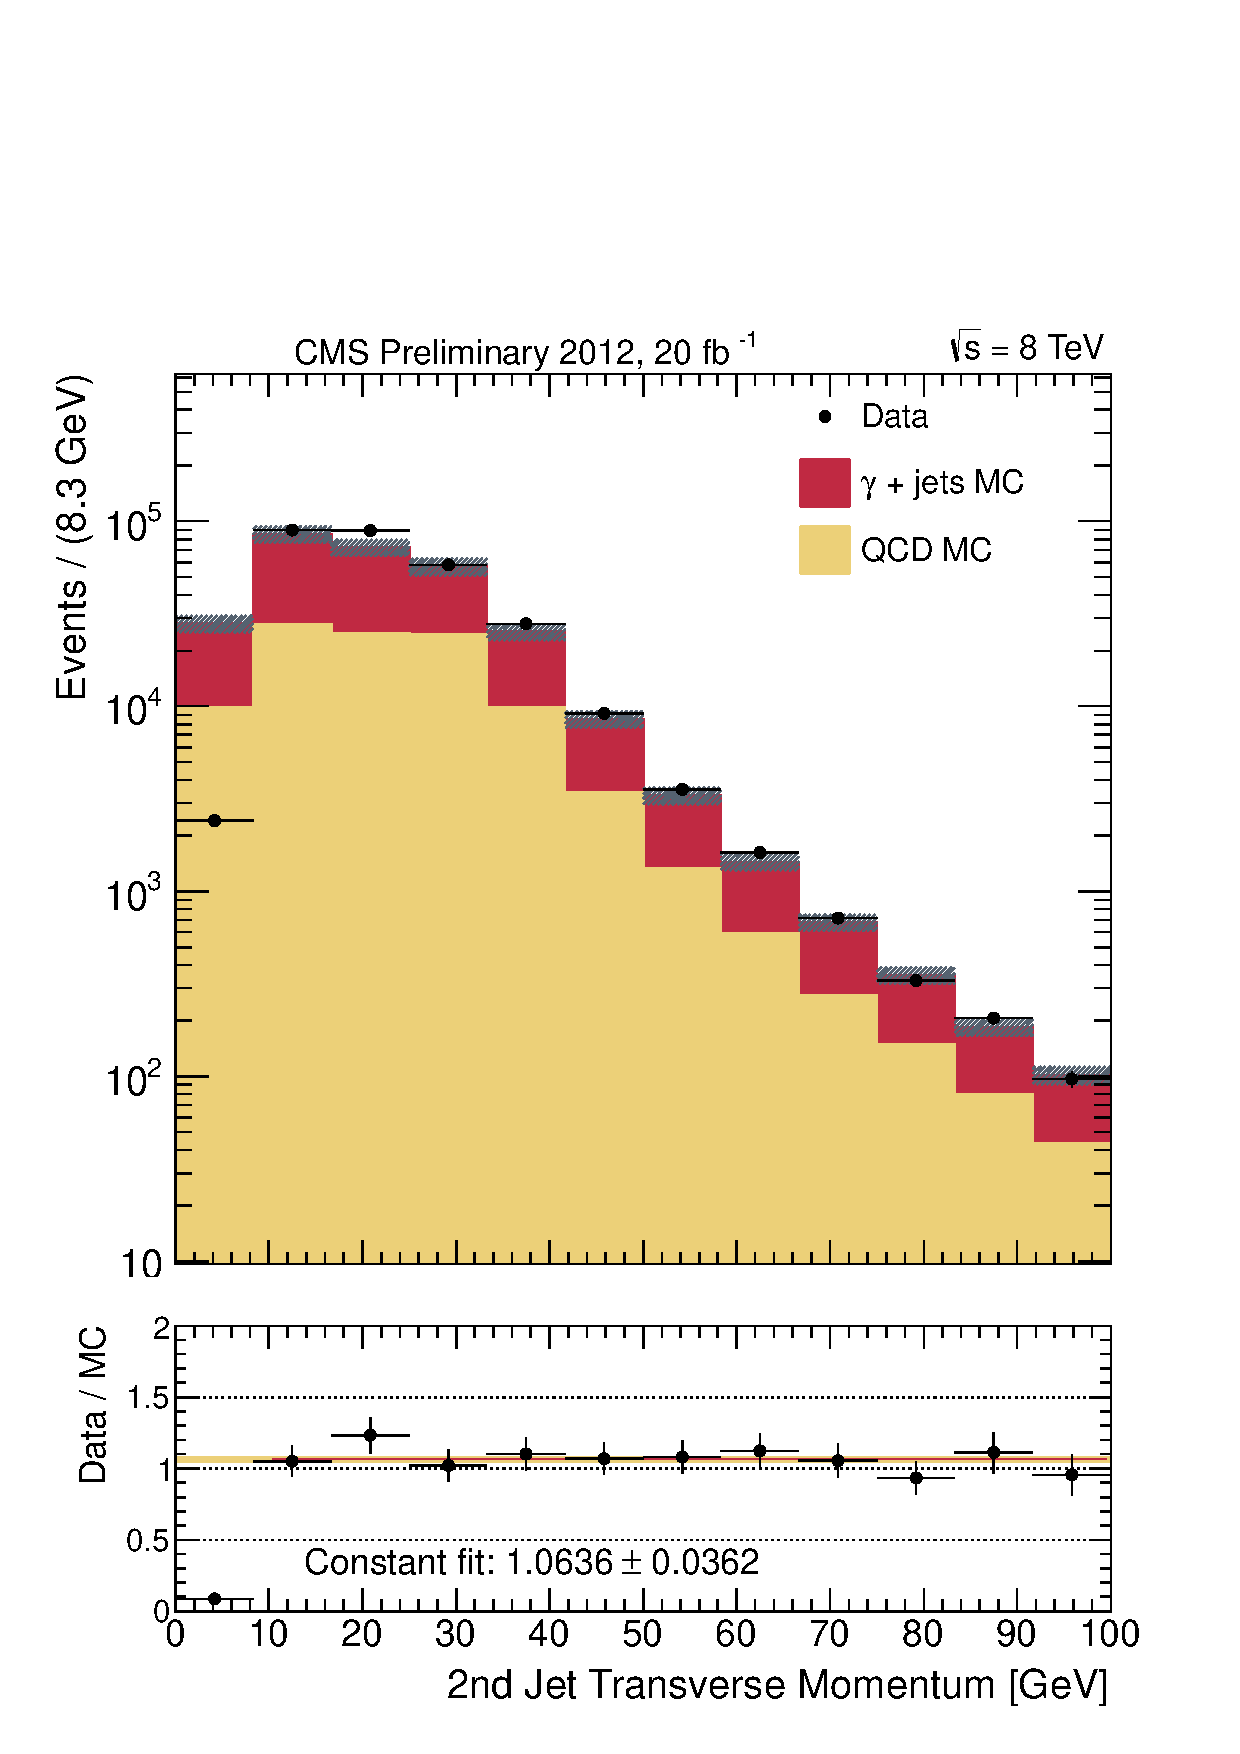
\includegraphics[width=0.45\textwidth]{chapitre4/figs/ptSecondJet_passedID_log.pdf}}\hfill
    \subcaptionbox{\label{met}}[0.45\textwidth]{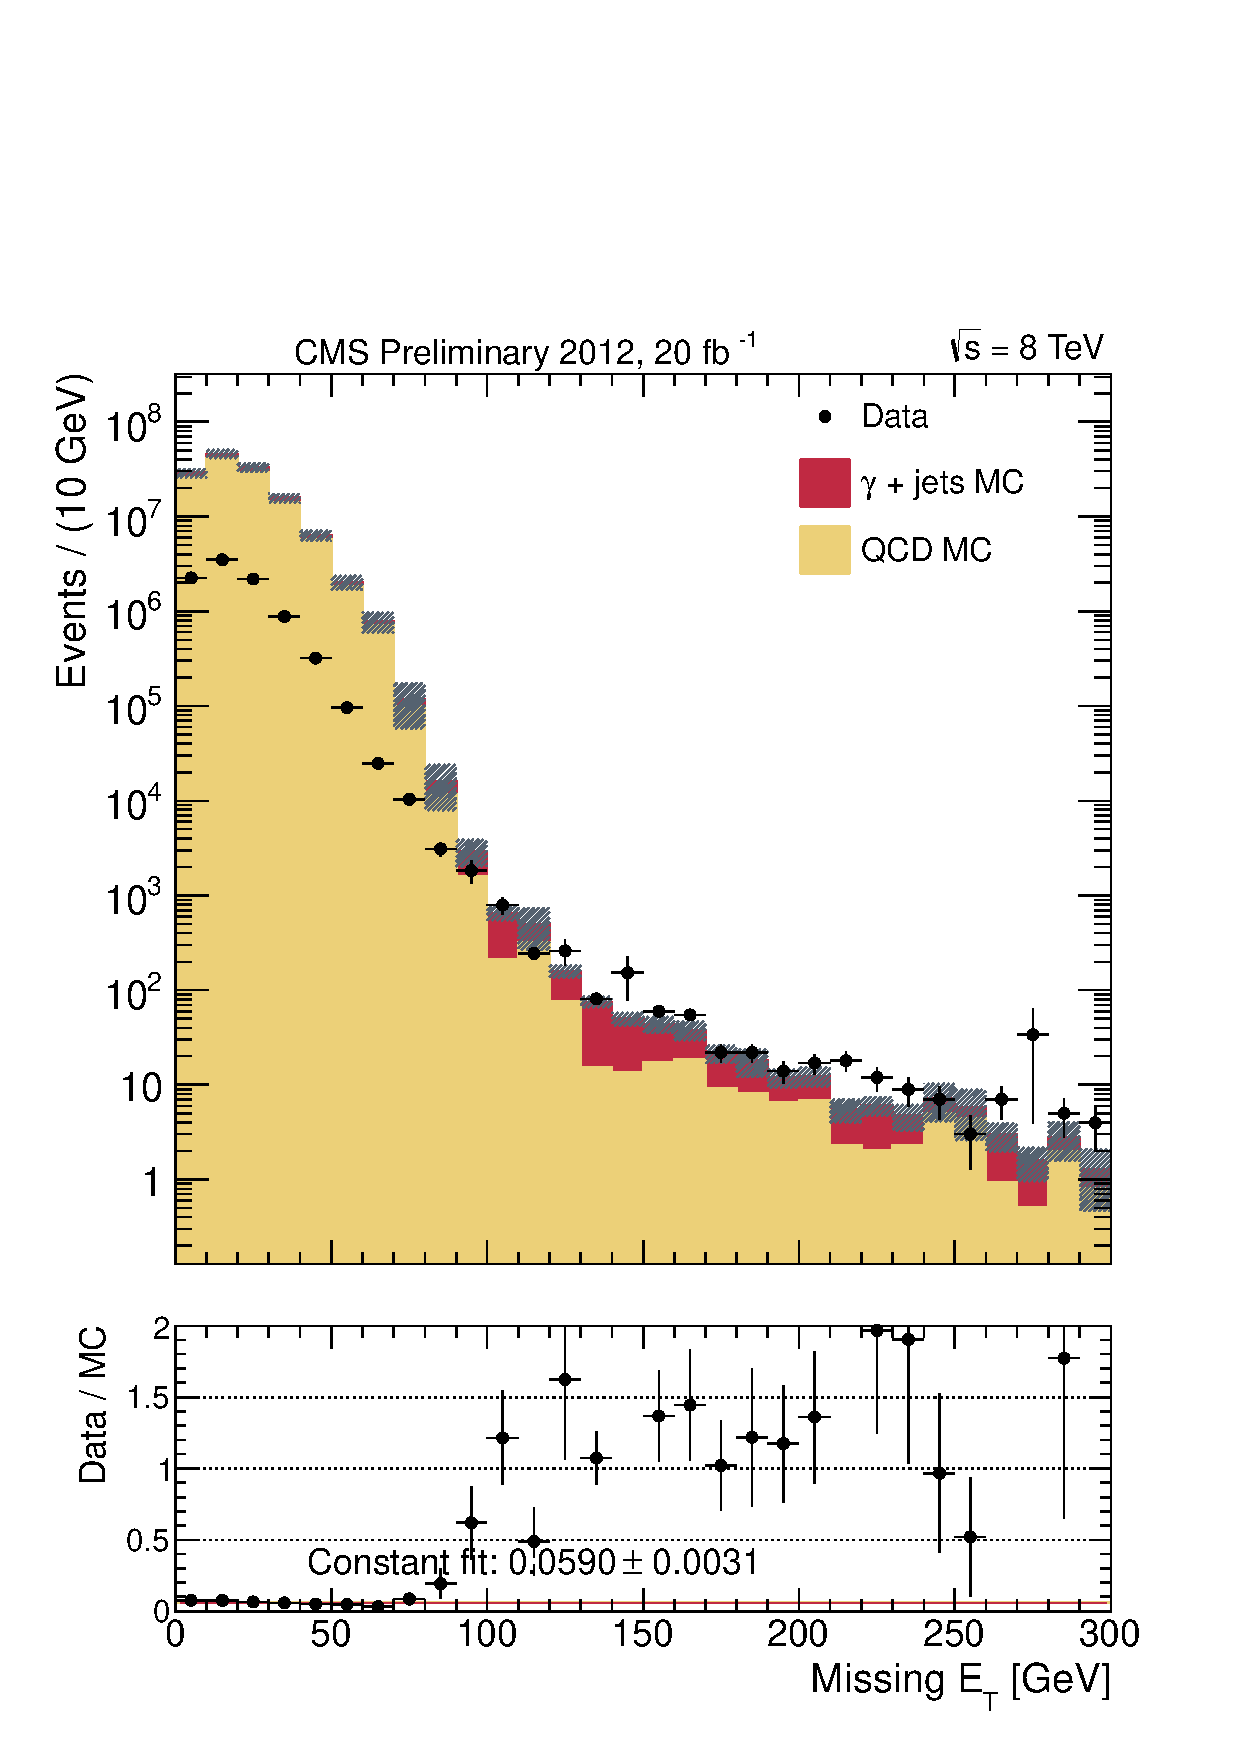
\includegraphics[width=0.45\textwidth]{chapitre4/figs/MET_passedID_log.pdf}}
    \caption{Comparaison entre la simulation (histogrammes) et les données (points) de l'impulsion transverse pour le photon (\subref{pt_photon}), pour le premier jet de l'événement (\subref{pt_first_jet}), le second (\subref{pt_second_jet}) ainsi que pour l'énergie transverse manquante (\subref{met}) après sélection. Une coupure additionnelle sur l'impulsion transverse du photon à \SI{175}{\GeV} a été appliquée pour éviter les effets de \emph{préscales} des différents chemins de déclenchement (plus de détails \cref{sec:jetmet_strategy}).}
    \label{fig:pt_photon_jet}
\end{figure}

\bigskip

Sur les données, on demande à ce que les événements aient déclenchés les chemins de déclenchement demandant un bon photon isolé. Plusieurs chemins de déclenchement existent suivant l'impulsion du photon demandée, dont la plupart préscalés. Afin de pouvoir comparer les données et la simulation sans être gêné par le préscale, on applique une coupure supplémentaire sur l'impulsion transverse du photon à \SI{175}{\GeV}. Cette coupure n'est pas appliquée pour déterminer les facteurs de corrections, mais uniquement pour comparer les distributions.

\smallskip

Finalement, la simulation des événements QCD et $\gamma$ + jets a été effectuée pendant la prise de données. À cette époque, le profil de \pu n'était pas encore connu précisément. Ainsi, une estimation de ce profil a été utilisé pour la simulation. On repondère donc le profil de \pu de la simulation pour qu'il corresponde à celui observé sur les données collectées.

\subsection{Stratégie d'analyse} \label{sec:jetmet_strategy}

On effectue un découpage suivant l'impulsion transverse du photon et de sa position angulaire, afin d'augmenter la sensibilité de l'analyse. Pour l'impulsion transverse, on définit 14 classes :

\setlength{\columnsep}{0pt}
\begin{multicols}{4}
  \begin{itemize} \setlength{\itemsep}{0.4\itemsep}
      \item 40 - \SI{50}{\GeV}
      \item 50 - \SI{60}{\GeV}
      \item 60 - \SI{75}{\GeV}
      \item 100 - \SI{125}{\GeV}
      \item 125 - \SI{155}{\GeV}
      \item 155 - \SI{180}{\GeV}
      \item 180 - \SI{210}{\GeV}
      \item 250 - \SI{300}{\GeV}
      \item 300 - \SI{350}{\GeV}
      \item 350 - \SI{400}{\GeV}
      \item 400 - \SI{500}{\GeV}
      \item 500 - \SI{600}{\GeV}
      \item 600 - \SI{800}{\GeV}
      \item 800 - \SI{5000}{\GeV}
  \end{itemize}
\end{multicols}

À \SI{8}{\TeV} et à l'arbre, un processus $\Pphoton$ + 2 jets a une section efficace de \SI{45291 \pm 167}{\pb}. À cause des contraintes liées au système de déclenchement, on comprend que, à cause de la section efficace relativement élevé du processus, les chemins de déclenchement demandant simplement un bon photon soient hautement préscalés. En effet, le premier chemin de déclenchement non préscalé demande un photon d'au moins \SI{150}{\GeV}, et les chemins avec des critères plus lâches sur l'impulsion du photon sont eux préscalés. Afin d'éviter tout biais possible dans l'analyse, chaque classe en \ptg{} a été choisie de façon à être associée de façon exclusive à un chemin de déclenchement précis, tout en ayant, si possible, une efficacité de déclenchement maximale. Par exemple, pour la classe 100 - \SI{125}{\GeV}, on demande à ce que l'événement ait déclenché le chemin demandant un photon d'au moins \SI{90}{\GeV} (\texttt{HLT\_Photon90}). Les \SI{10}{\GeV} de différence entre le seuil du déclencheur et la classe en \pt permettent de tenir compte des possibles corrections en énergie entre le photon reconstruit au niveau HLT et le photon \pf, mais surtout d'éviter la courbe de \emph{turn-on} du déclencheur, et maximiser ainsi l'efficacité de déclenchement. À partir de \SI{155}{\GeV} (ou \SI{180}{\GeV} pour une période spécifique de prise de données), tous les événements sont requis d'avoir déclenché le premier chemin non-préscalé. On présente \cref{tab:triggers_jetmet} les chemins de déclenchement associés à chaque classe en \ptg. Les chemins de déclenchement ayant changé pendant la période de prise de données (notamment avec l'apparition puis la disparition du déclencheur \texttt{HLT\_Photon150}), deux tableaux sont présents, un pour chaque période de prise de données.

\begin{table} \centering
  \subcaptionbox{Run ACD\label{tab:triggers_runACD}}[0.45\textwidth]{
  \begin{tabular}{@{}cc@{}} \toprule
    Classes en \ptg & Déclencheurs \\ \midrule
    40 - \SI{60}{\GeV} & \texttt{HLT\_Photon30} \\
    60 - \SI{100}{\GeV} & \texttt{HLT\_Photon50} \\
    100 - \SI{155}{\GeV} & \texttt{HLT\_Photon90} \\
    155 - $\inf$ & \texttt{HLT\_Photon135} \\ \bottomrule
  \end{tabular}
  } \qquad
  \subcaptionbox{Run B\label{tab:triggers_runB}}[0.45\textwidth]{
  \begin{tabular}{@{}cc@{}} \toprule
    Classe en \ptg & Déclencheurs \\ \midrule
    40 - \SI{60}{\GeV} & \texttt{HLT\_Photon30} \\
    60 - \SI{100}{\GeV} & \texttt{HLT\_Photon50} \\
    100 - \SI{155}{\GeV} & \texttt{HLT\_Photon90} \\
    155 - \SI{180}{\GeV} & \texttt{HLT\_Photon135} \\
    180 - $\inf$ & \texttt{HLT\_Photon150} \\ \bottomrule
  \end{tabular}}
  \caption{Chemins de déclenchement associés aux classes en \ptg, pour deux périodes de prises de données correspondantes à des conditions de déclenchement différentes.}
  \label{tab:triggers_jetmet}
\end{table}

Les préscales des chemins de déclenchement vont aussi affecter les distributions de \pu associées. Ainsi, lors de la procédure de repondération du \pu sur la simulation, il faut tenir compte du déclencheur associé à l'événement. En fonction de l'impulsion transverse du photon, on détermine quel chemin de déclenchement l'événement a dû déclencher sur les données pour passer la sélection, et on utilise cette information pour obtenir le profil de \pu correspondant. On présente \cref{fig:pu_jetmet} une comparaison entre deux profils de \pu, obtenus pour deux chemins de déclenchement différents. On voit très clairement la différence entre les deux profils.

\begin{figure}[tbp]
    \centering
    \includegraphics[width=0.5\textwidth]{chapitre4/figs/pu_plot.pdf}
    \caption{Distribution du nombre moyen d'interactions par croisement de faisceaux pour deux chemins de déclenchement, \texttt{HLT\_Photon30} (rouge) et \texttt{HLT\_Photon150} (bleu)}
    \label{fig:pu_jetmet}
\end{figure}

\bigskip

En $\aeta$, on procède à un découpage en 7 classes :

\begin{multicols}{4}
  \begin{itemize} \setlength{\itemsep}{0.4\itemsep}
      \item \num{0} - \num{0.8}
      \item \num{0.8} - \num{1.3}
      \item \num{1.3} - \num{1.9}
      \item \num{1.9} - \num{2.5}
      \item \num{2.5} - \num{3}
      \item \num{3} - \num{3.2}
      \item \num{3.2} - \num{5.2}
  \end{itemize}
\end{multicols}

Pour chaque classe en $p_T^{\gamma}$ et $\aeta$, on calcule la réponse en utilisant la méthode de la balance et la méthode MPF, sur les données et sur la simulation. On présente \cref{fig:responses_mpf_balancing} les distributions des réponses obtenues pour les deux méthodes, pour diverses classes en \pt, et pour $\aeta < \num{1.3}$. Pour chaque classe, on extrait la réponse moyenne $R_m$, définie comme la moyenne de la distribution des réponses, ainsi que la résolution $\sigma$, définie comme la moyenne quadratique de la distribution des réponses (RMS) divisée par $R_m$. Sur chaque distribution représentée \cref{fig:responses_mpf_balancing}, les réponses moyennes sont représentées par une ligne noire pour les données, et par une ligne bleue pour la simulation. On constate que ces réponses sont différentes, et c'est ce biais que l'on souhaite corriger en appliquant les corrections résiduelles.

\begin{figure}[p]
    \centering
    \subcaptionbox{\label{fig:bal_eta013_pt_125_155}}[0.45\textwidth]{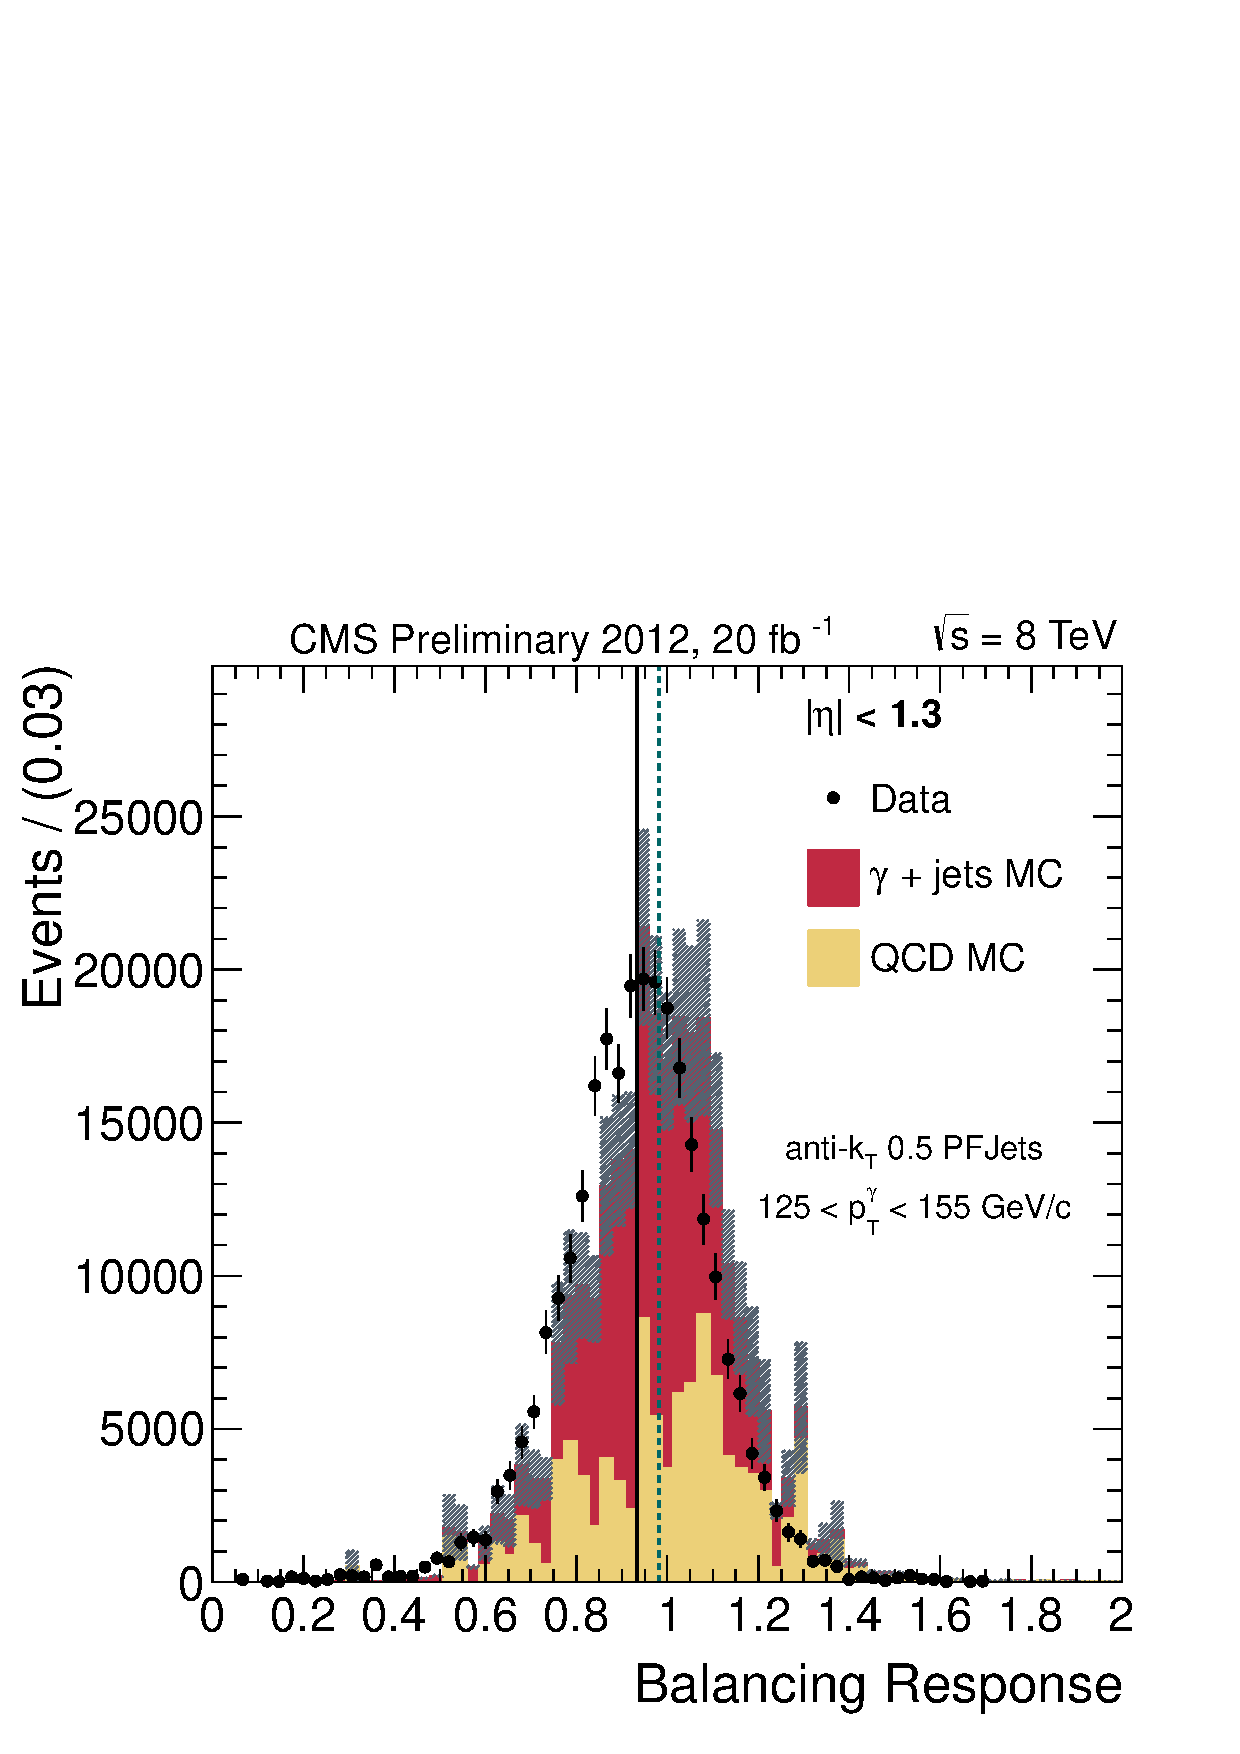
\includegraphics[width=0.45\textwidth]{chapitre4/figs/resp_balancing_eta013_ptPhot_125_155.pdf}}\hfill
    \subcaptionbox{\label{fig:bal_eta013_pt_210_250}}[0.45\textwidth]{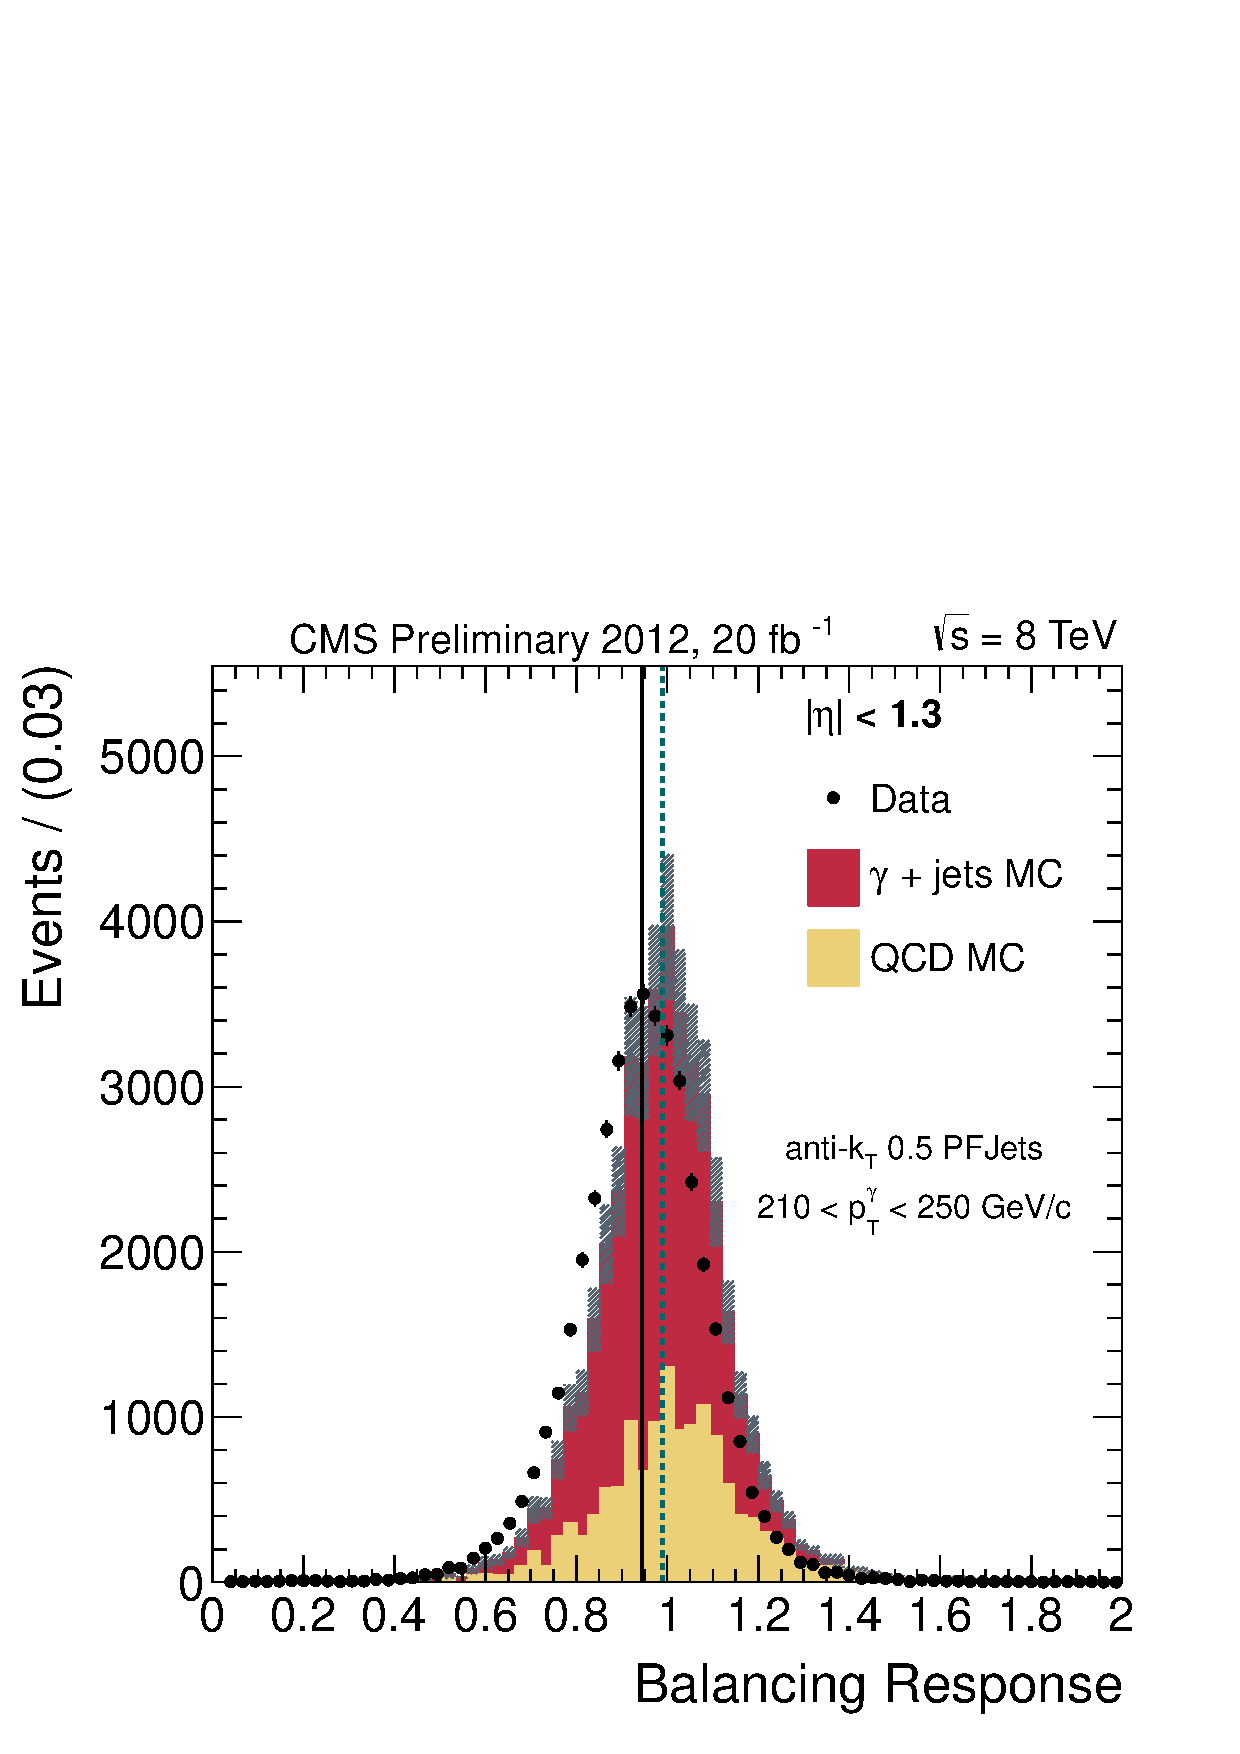
\includegraphics[width=0.45\textwidth]{chapitre4/figs/resp_balancing_eta013_ptPhot_210_250.pdf}}
    \subcaptionbox{\label{fig:mpf_eta013_pt_125_155}}[0.45\textwidth]{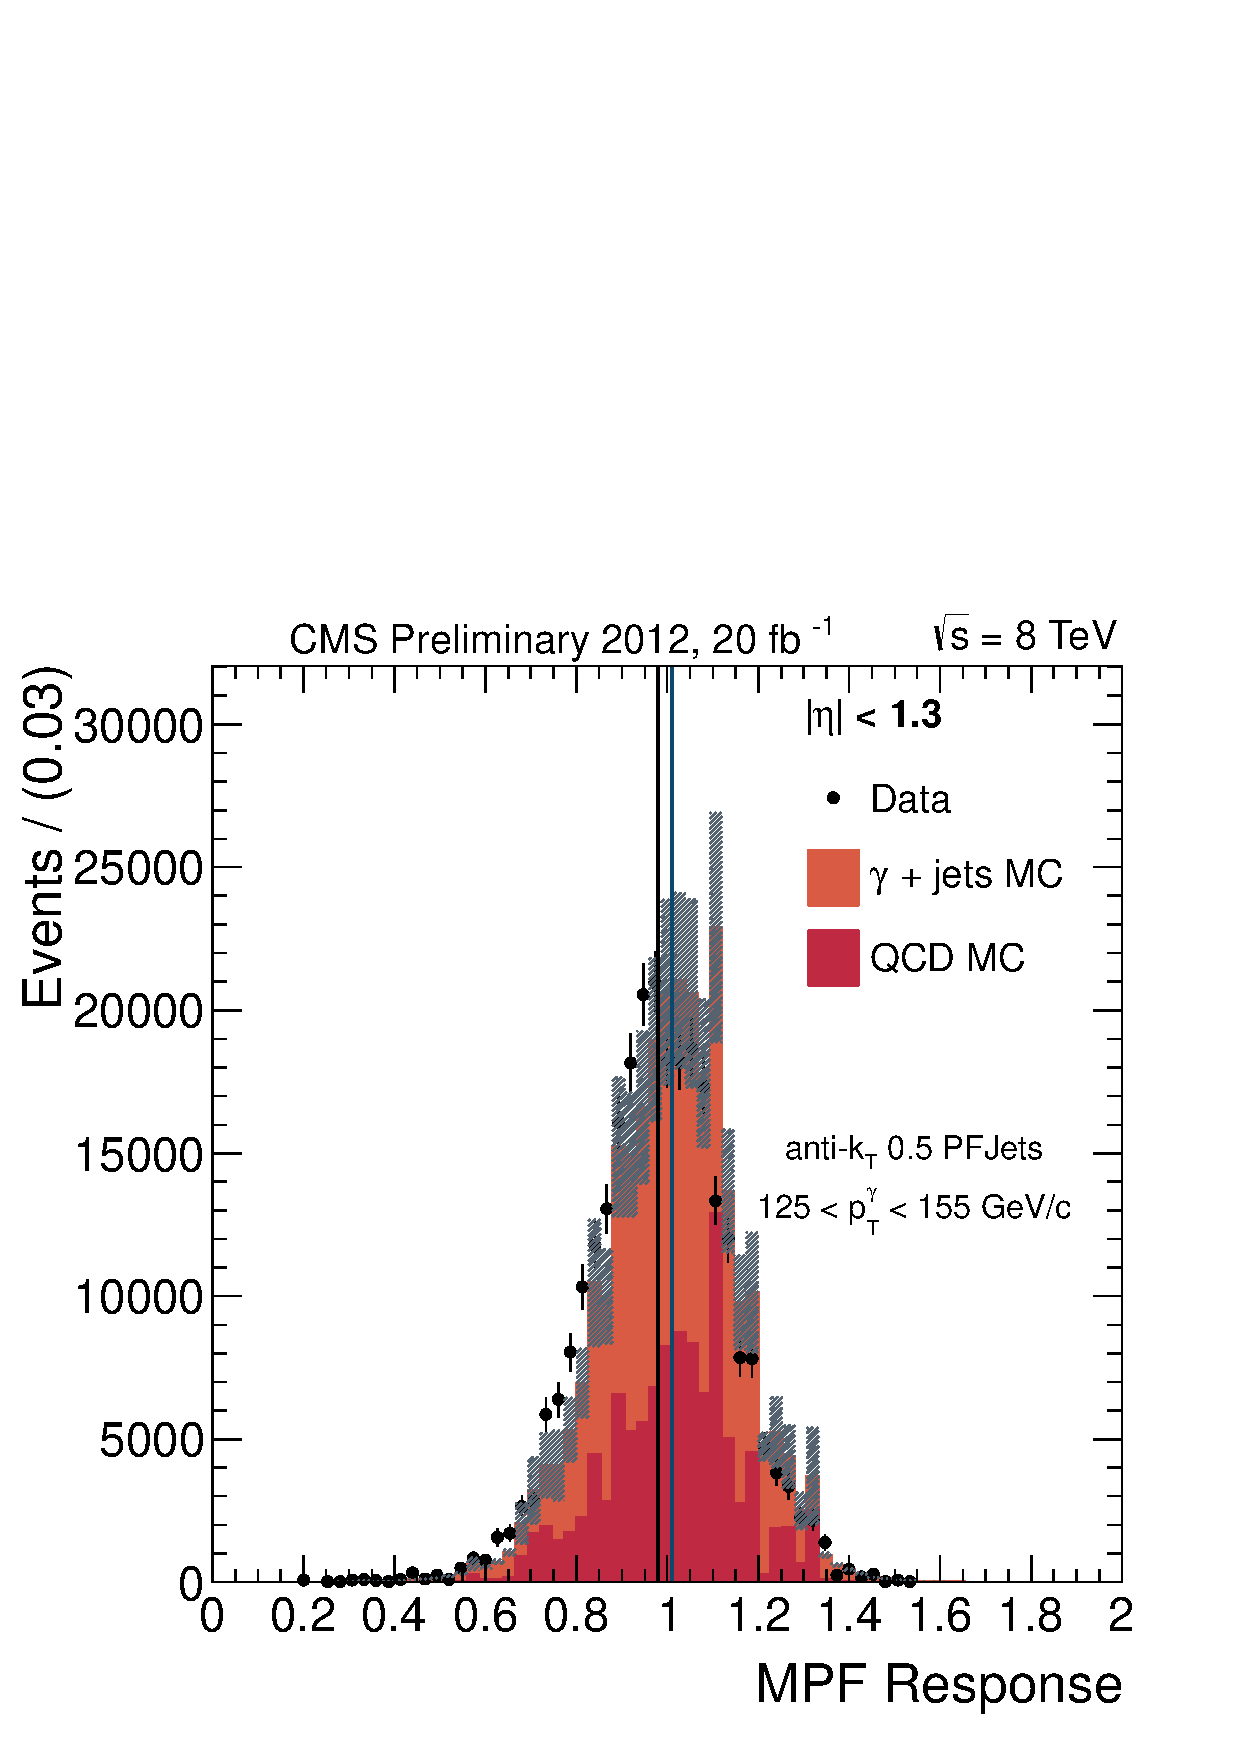
\includegraphics[width=0.45\textwidth]{chapitre4/figs/resp_mpf_eta013_ptPhot_125_155.pdf}}\hfill
    \subcaptionbox{\label{fig:mpf_eta013_pt_210_250}}[0.45\textwidth]{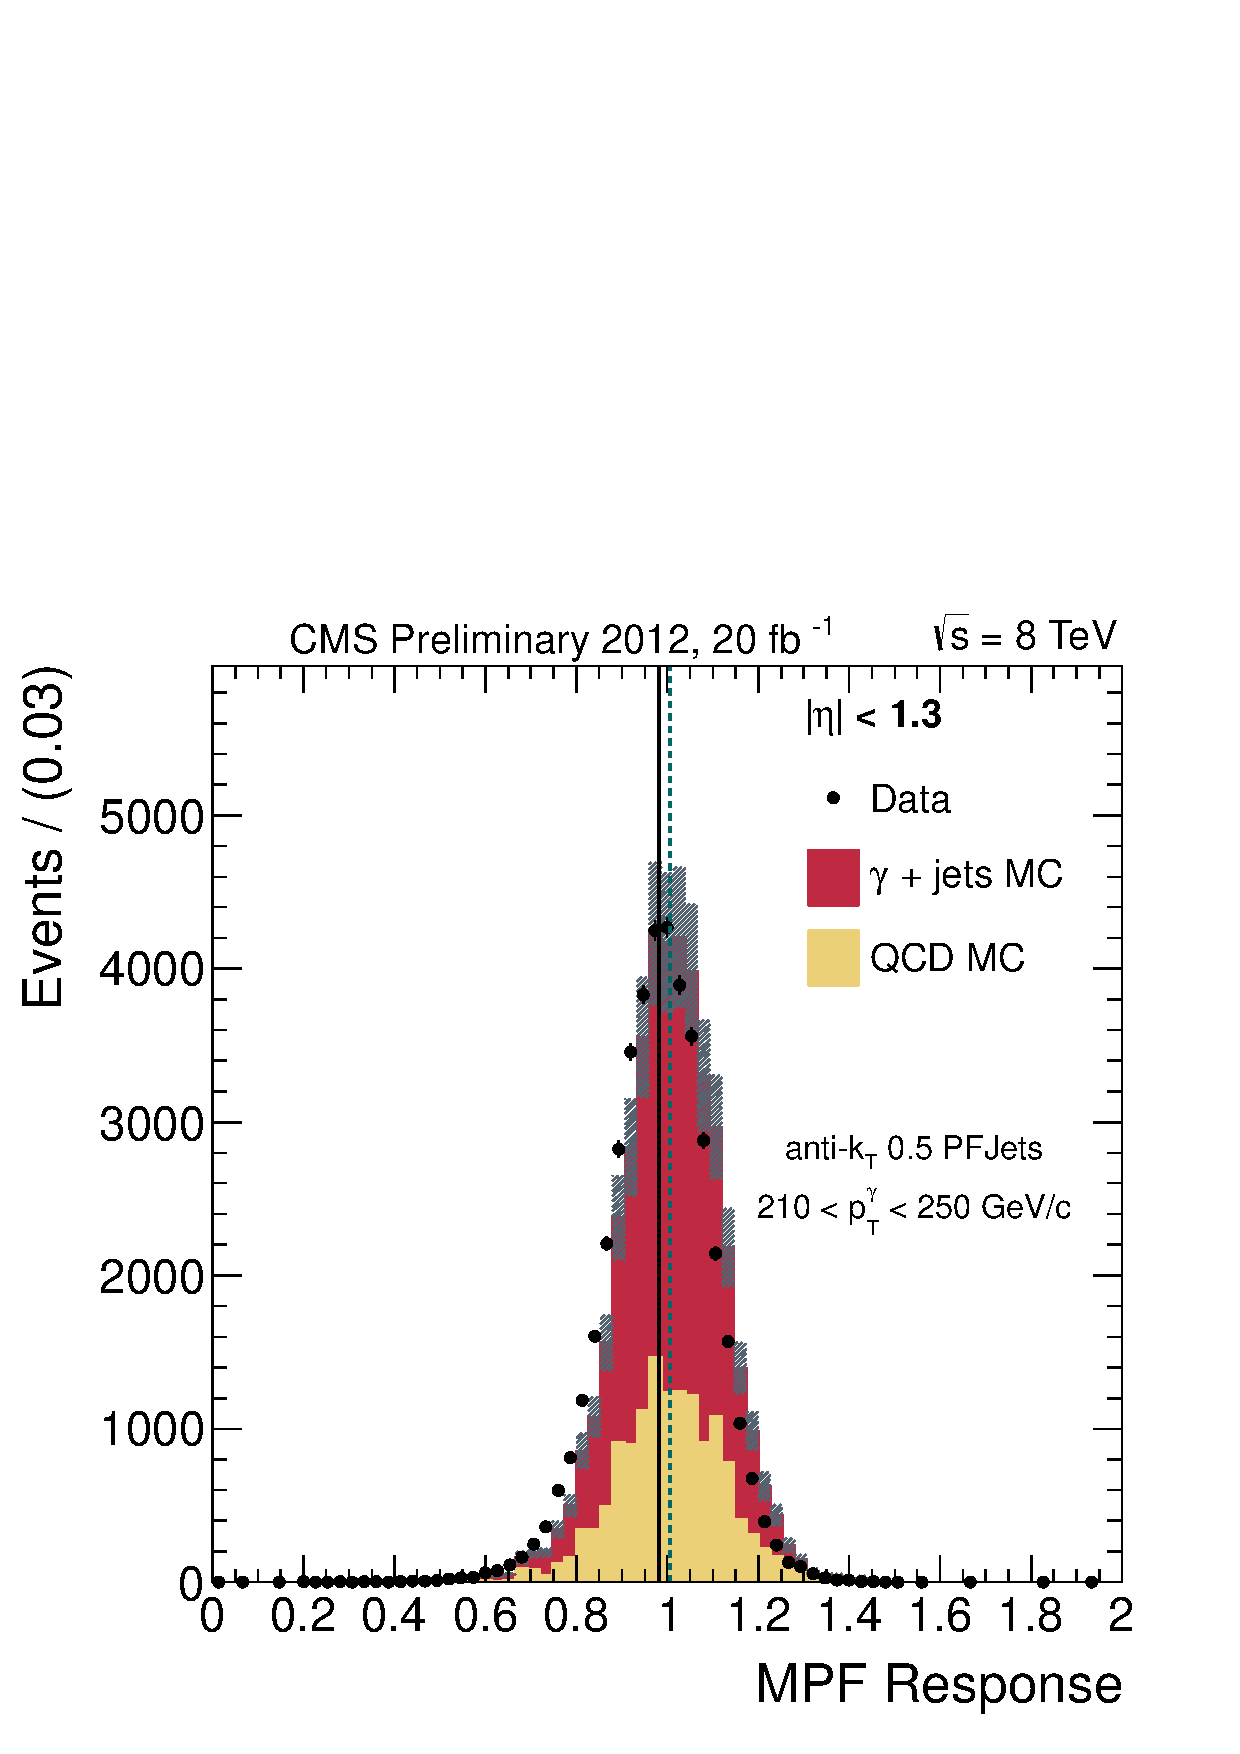
\includegraphics[width=0.45\textwidth]{chapitre4/figs/resp_mpf_eta013_ptPhot_210_250.pdf}}
    \caption{Réponses pour la méthode de la balance (haut) et pour la méthode MPF (bas), pour deux classes en \pt : 125 - \SI{155}{\GeV} (gauche) et 210 - \SI{250}{\GeV} (droite). Pour toutes les distributions, $\aeta < \num{1.3}$. Les histogrammes représentent la simulation et les points les données. La ligne noire correspond à la réponse moyenne $R_m$ extraite sur les données et la ligne bleue celle extraite sur la simulation.}
    \label{fig:responses_mpf_balancing}
\end{figure}

\subsection{Résultats}

Pour chaque distribution des réponses, on extrait la réponse moyenne et la résolution. Afin d'extraire les corrections résiduelles, on trace l'évolution de $R_m$ en fonction de l'impulsion transverse du photon, pour les données et la simulation, pour différentes classes en \aeta. En calculant le rapport entre données et simulation, on détermine le facteur de correction à appliquer sur les données.

On définit le facteur de correction $f$ par
\begin{align*}
  f &= \frac{R_m^{\text{simulation}}}{R_m^{\text{données}}}
\end{align*}

En appliquant ce facteur de correction sur les données, on a
\begin{align*}
  f\;R_m^{\text{données}} &= R_m^{\text{simulation}}
\end{align*}
ce qui est effectivement le but recherché.

\bigskip

On présente par la suite les résultats obtenus avec les méthodes de la balance et MPF, avec et sans extrapolation, qui permettent d'extraire le facteur de correction résiduel. Pour chaque méthode, les distributions des réponses moyennes et des résolutions seront présentées pour différentes classes en \aeta.

\subsubsection{Méthode de la balance, sans extrapolation}

On présente \cref{fig:balancing_resp} les distributions des réponses moyennes pour différentes classes en \aeta. Le ratio entre les données et la simulation accompagne ces distributions, ce qui permet d'extraire les facteurs de corrections. Pour ce faire, une interpolation linéaire par une constante est dérivée à l'aide des divers ratios. On trouve aussi \cref{fig:balancing_reso} les distributions des résolutions pour les mêmes classes en \aeta. Même si ces résolutions ne sont pas utilisées pour dériver les corrections résiduelles, elles sont intéressantes pour se rendre compte des performances de reconstruction des algorithmes. On s'aperçoit d'ailleurs que les jets sont mieux reconstruits sur la simulation que sur les données. Cet effet donne lieu à une autre série de corrections pour la résolution, qui vise à dégrader la résolution des jets sur la simulation pour correspondre à celle des données.

\begin{figure}[p]
    \centering
    \subcaptionbox{\label{fig:bal_eta008}}[0.45\textwidth]{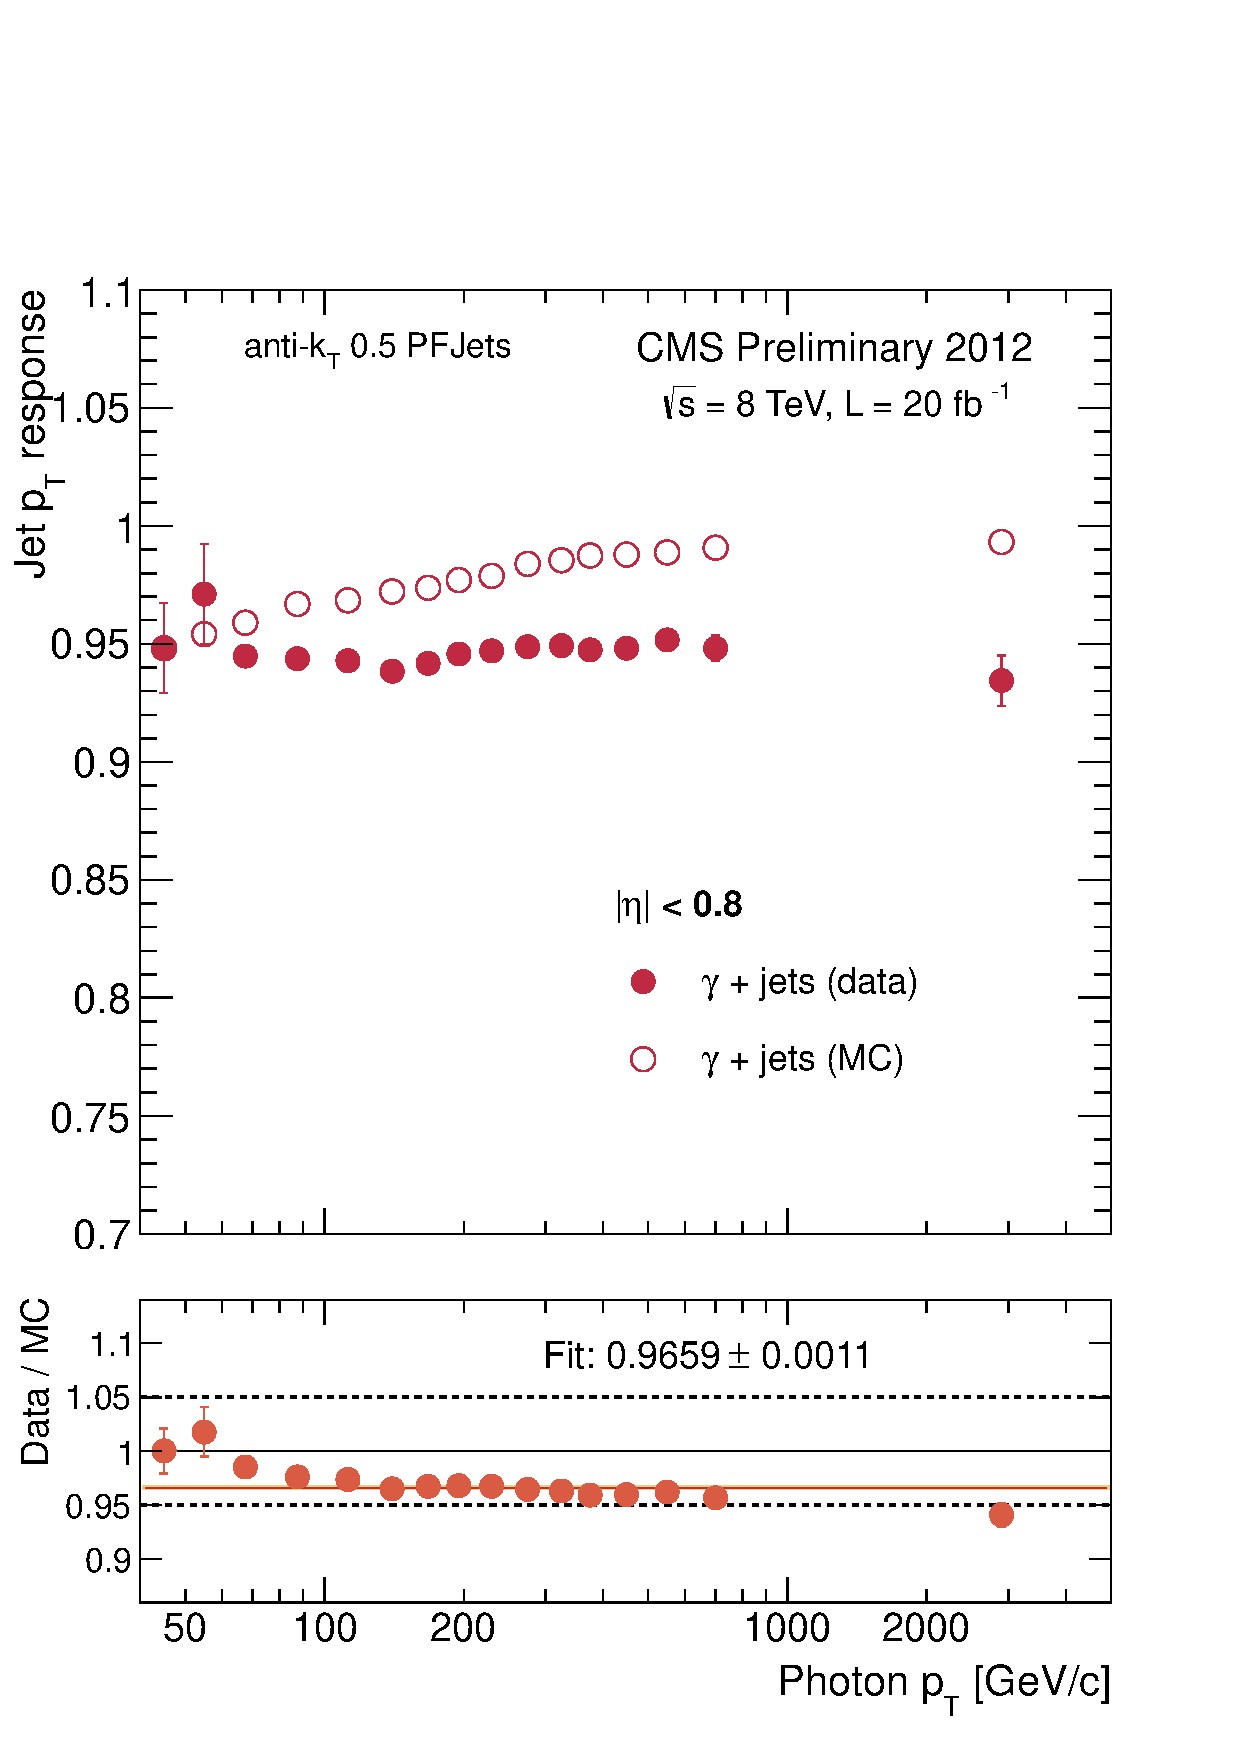
\includegraphics[width=0.45\textwidth]{chapitre4/figs/resp_balancing/response_eta008_balancing.pdf}}\hfill
    \subcaptionbox{\label{fig:bal_eta0813}}[0.45\textwidth]{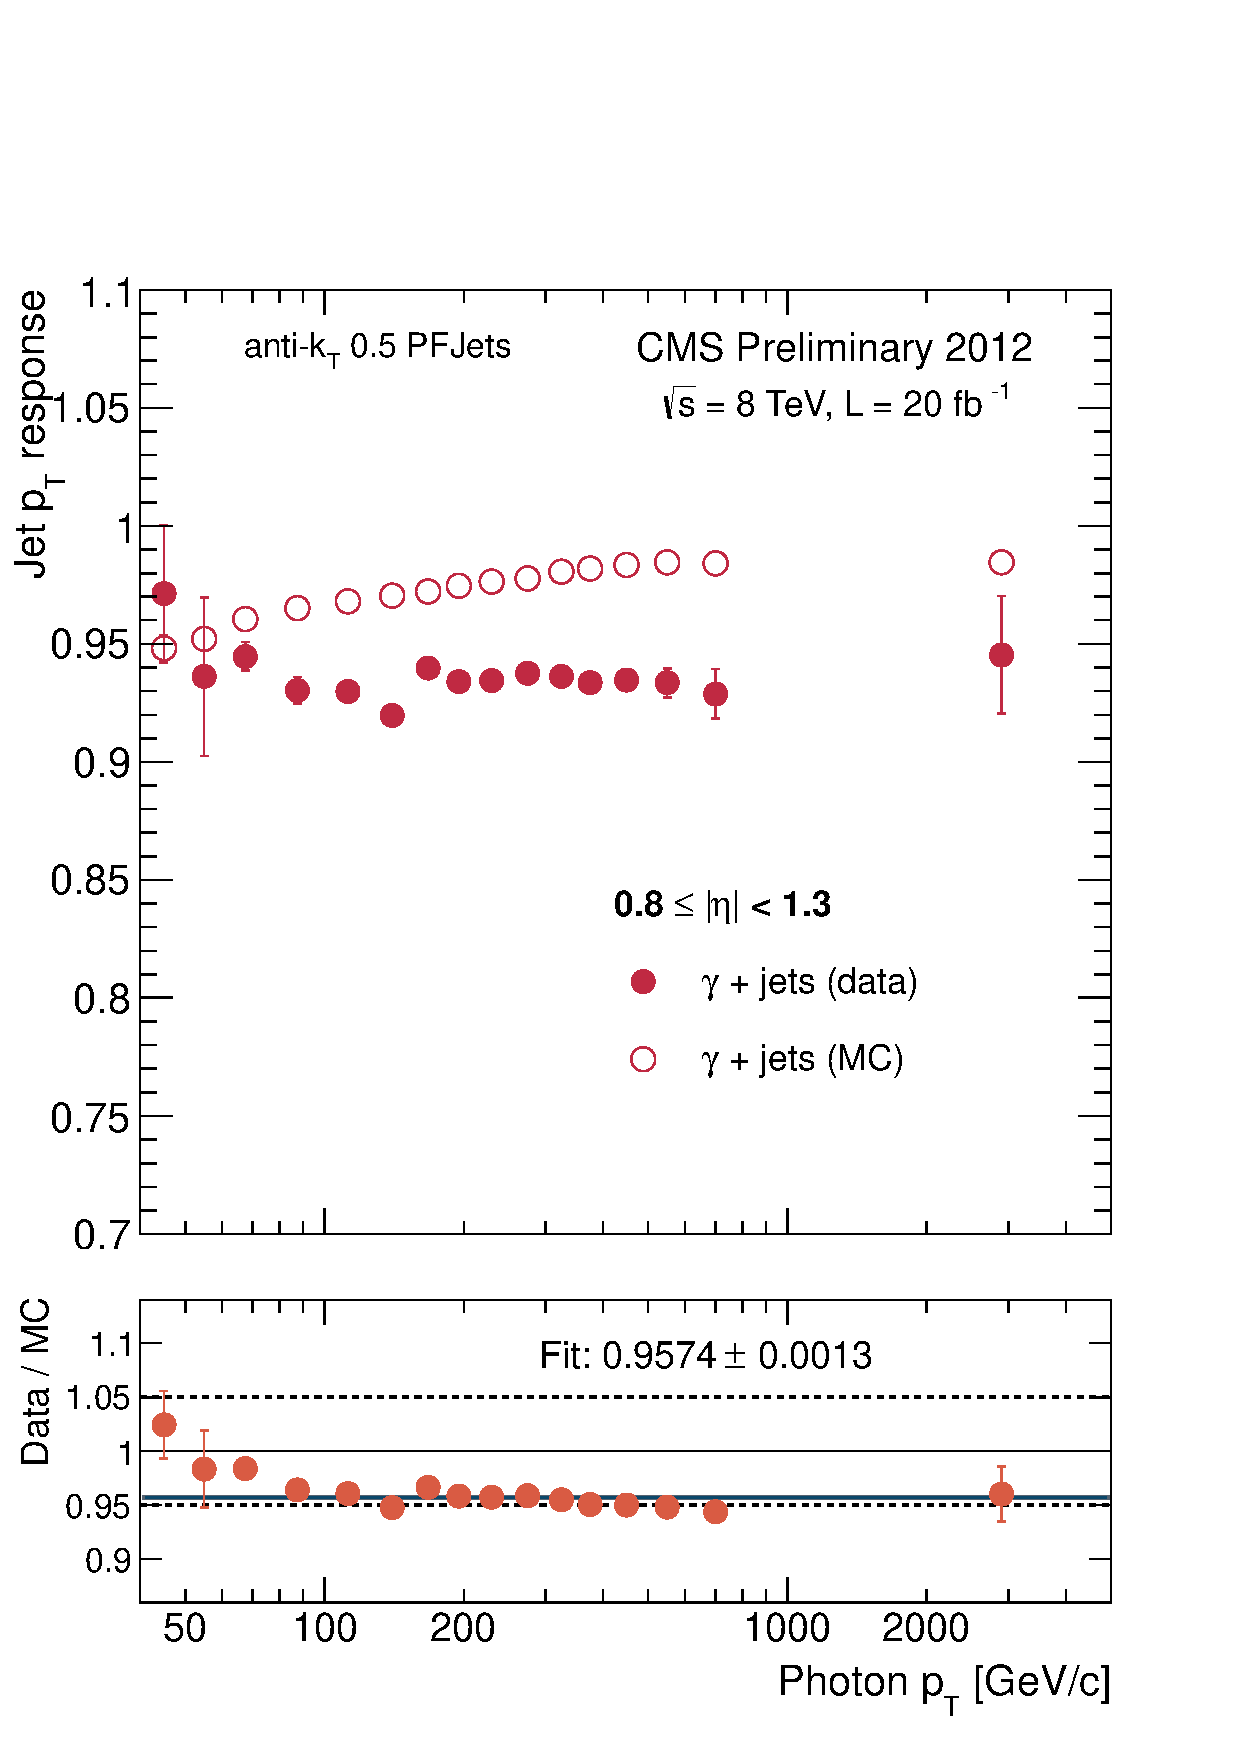
\includegraphics[width=0.45\textwidth]{chapitre4/figs/resp_balancing/response_eta0813_balancing.pdf}}
    \subcaptionbox{\label{fig:bal_eta1319}}[0.45\textwidth]{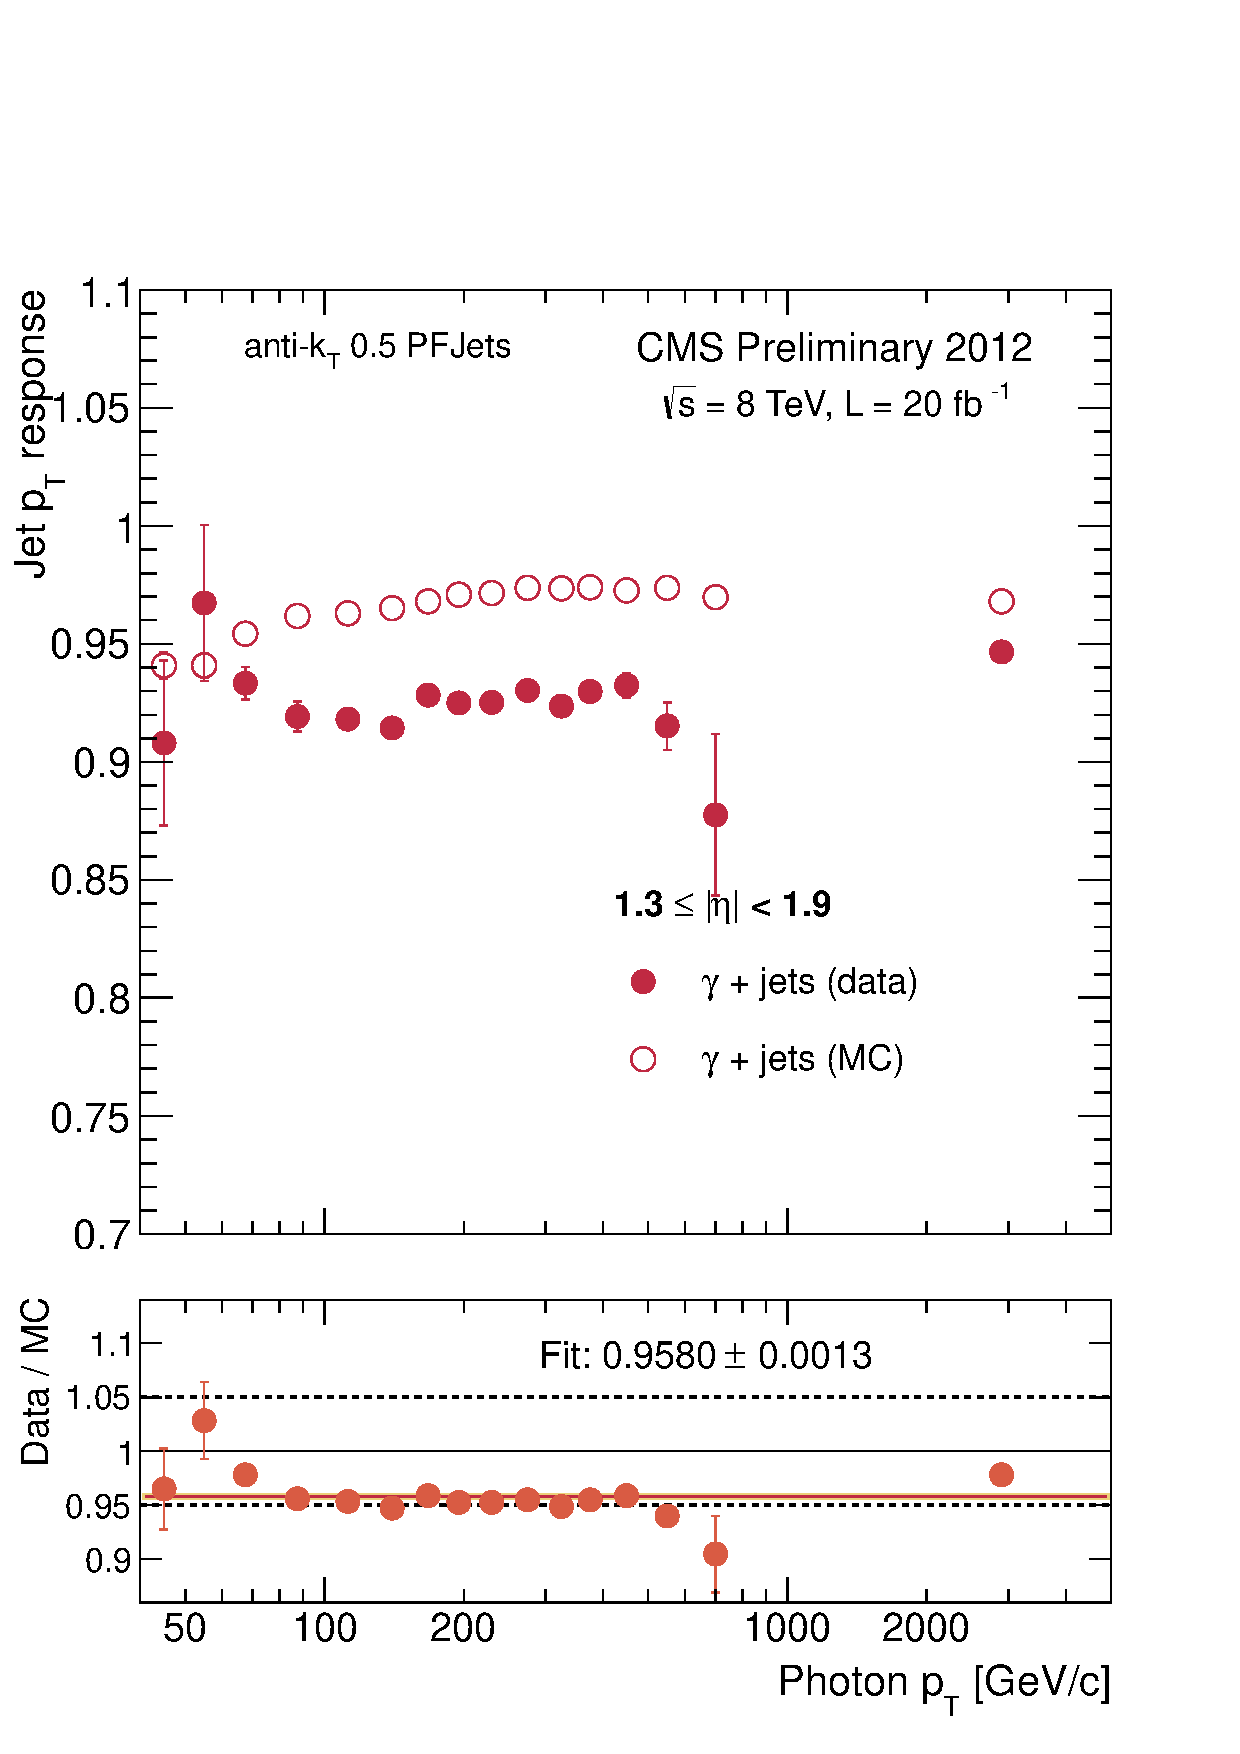
\includegraphics[width=0.45\textwidth]{chapitre4/figs/resp_balancing/response_eta1319_balancing.pdf}}\hfill
    \subcaptionbox{\label{fig:bal_eta1925}}[0.45\textwidth]{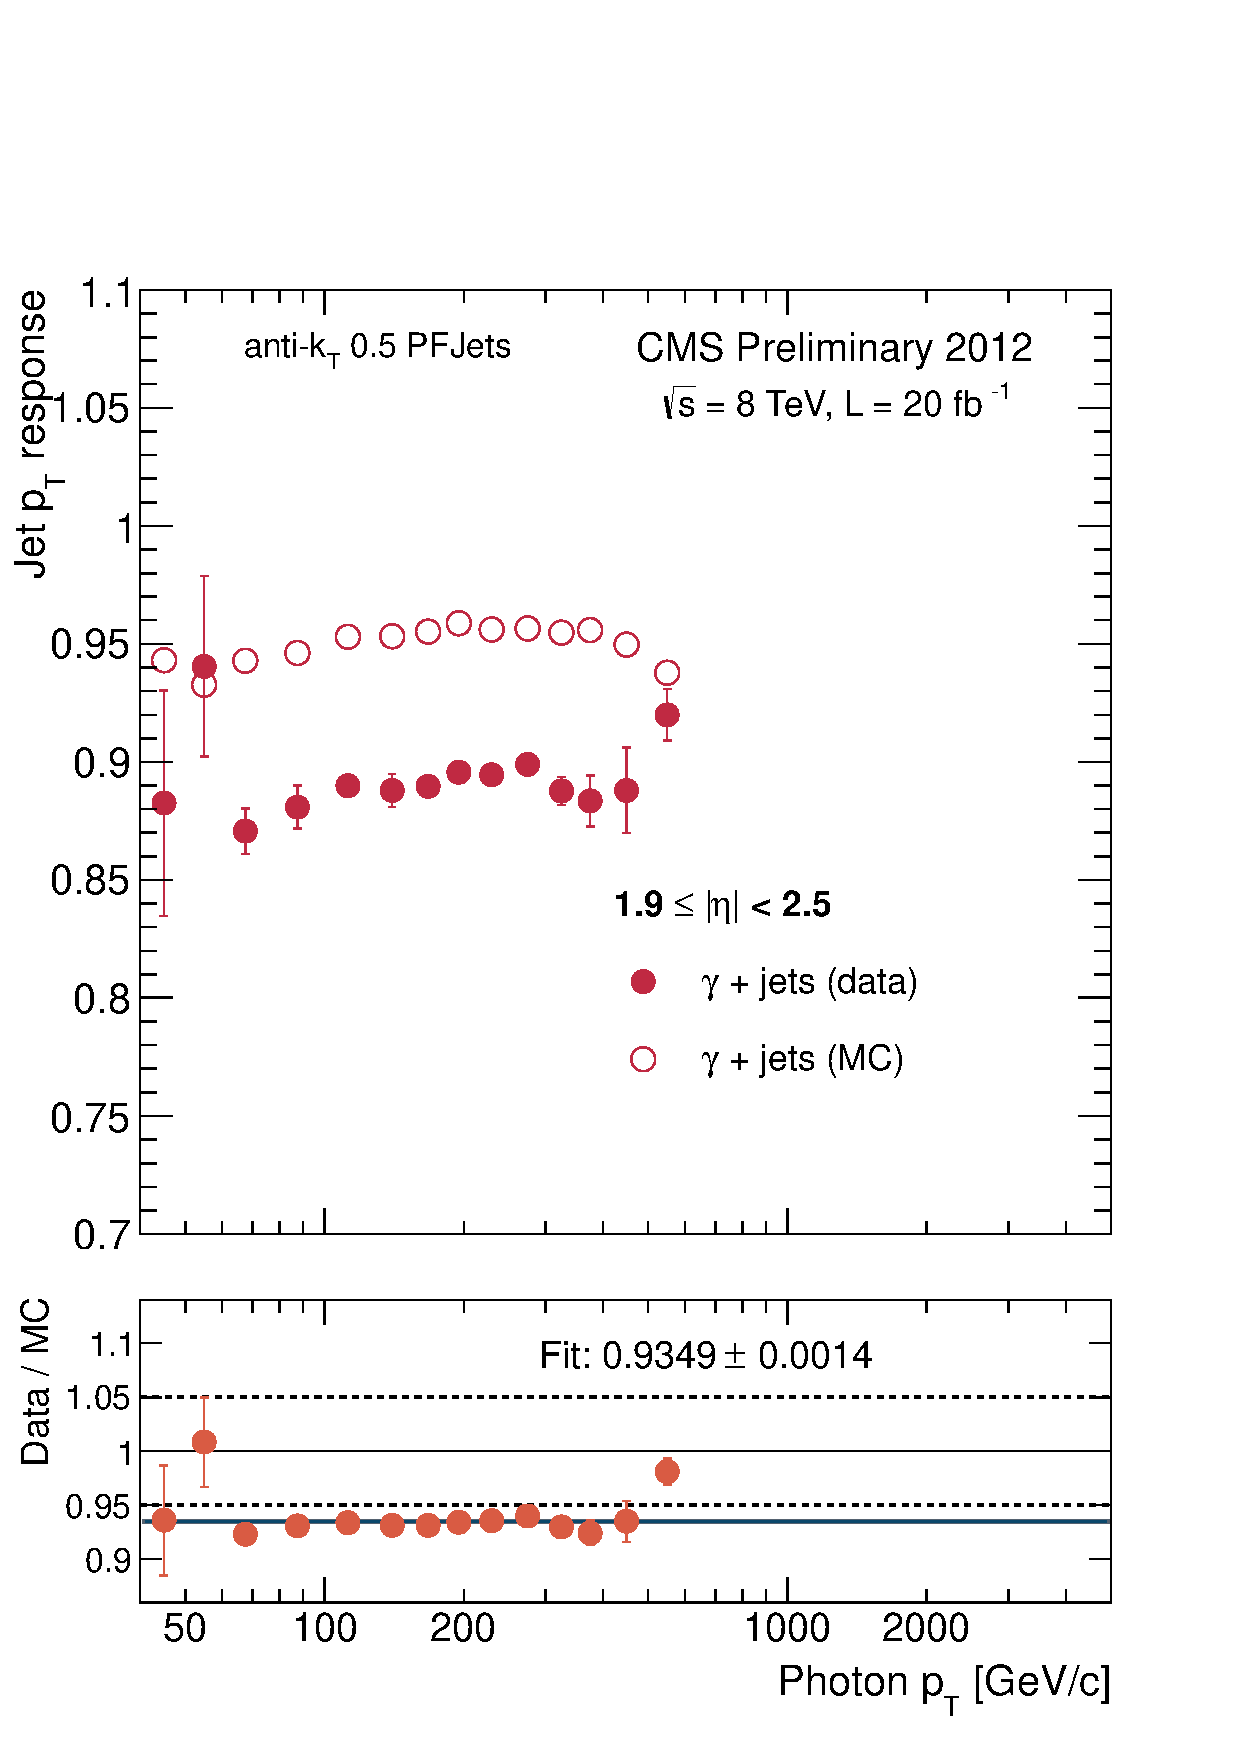
\includegraphics[width=0.45\textwidth]{chapitre4/figs/resp_balancing/response_eta1925_balancing.pdf}}
    \caption{Réponses moyennes pour la méthode de la balance pour $\aeta < \num{0.8}$ (\subref{fig:bal_eta008}), $\num{0.8} \leq \aeta < \num{1.3}$ (\subref{fig:bal_eta0813}), $\num{1.3} \leq \aeta < \num{1.9}$ (\subref{fig:bal_eta1319}), et $\num{1.9} \leq \aeta < \num{2.5}$ (\subref{fig:bal_eta1925}). Le ratio entre les données et la simulation est présenté sous chaque distribution, accompagné d'une interpolation linéaire constante (ligne grise).}
    \label{fig:balancing_resp}
\end{figure}

\begin{figure}[p]
    \centering
    \subcaptionbox{\label{fig:reso_bal_eta008}}[0.45\textwidth]{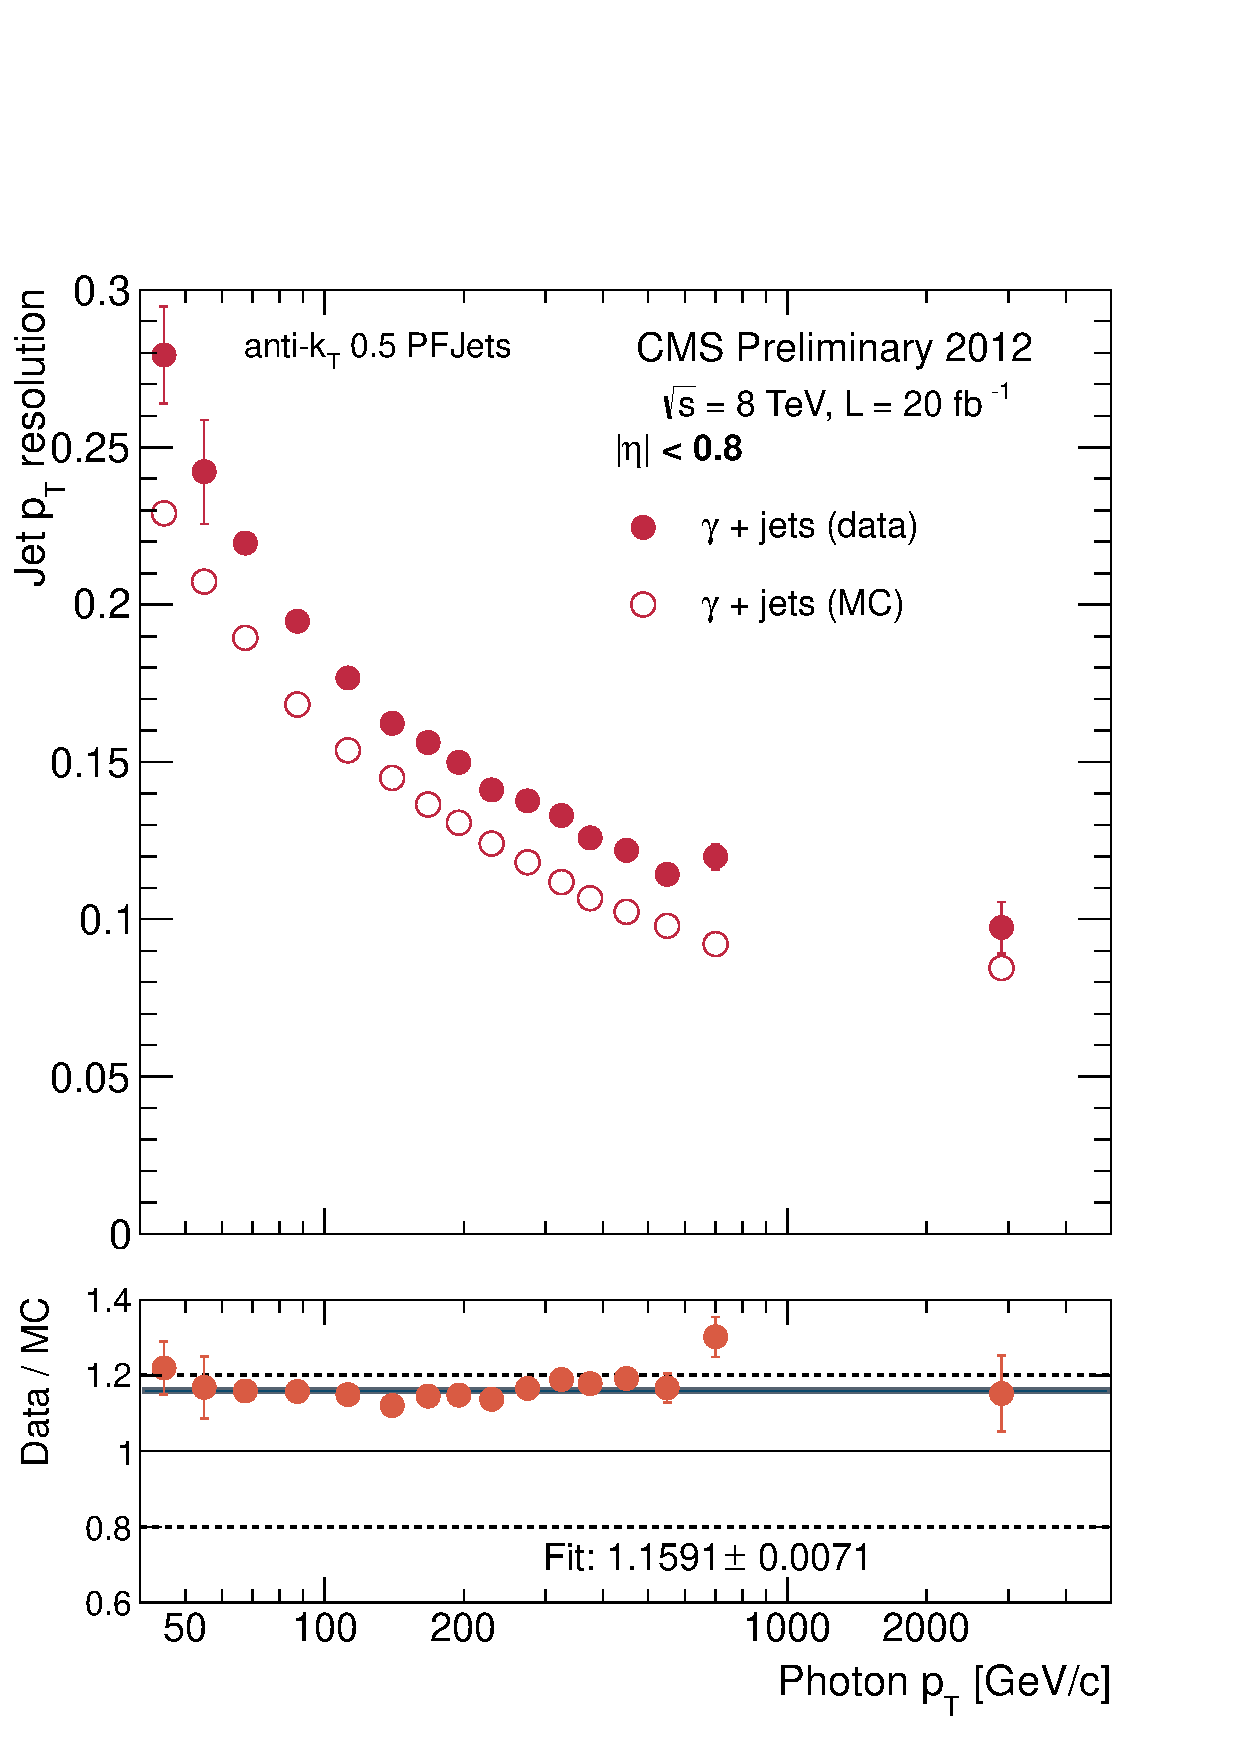
\includegraphics[width=0.45\textwidth]{chapitre4/figs/reso_balancing/resolution_eta008_balancing.pdf}}\hfill
    \subcaptionbox{\label{fig:reso_bal_eta0813}}[0.45\textwidth]{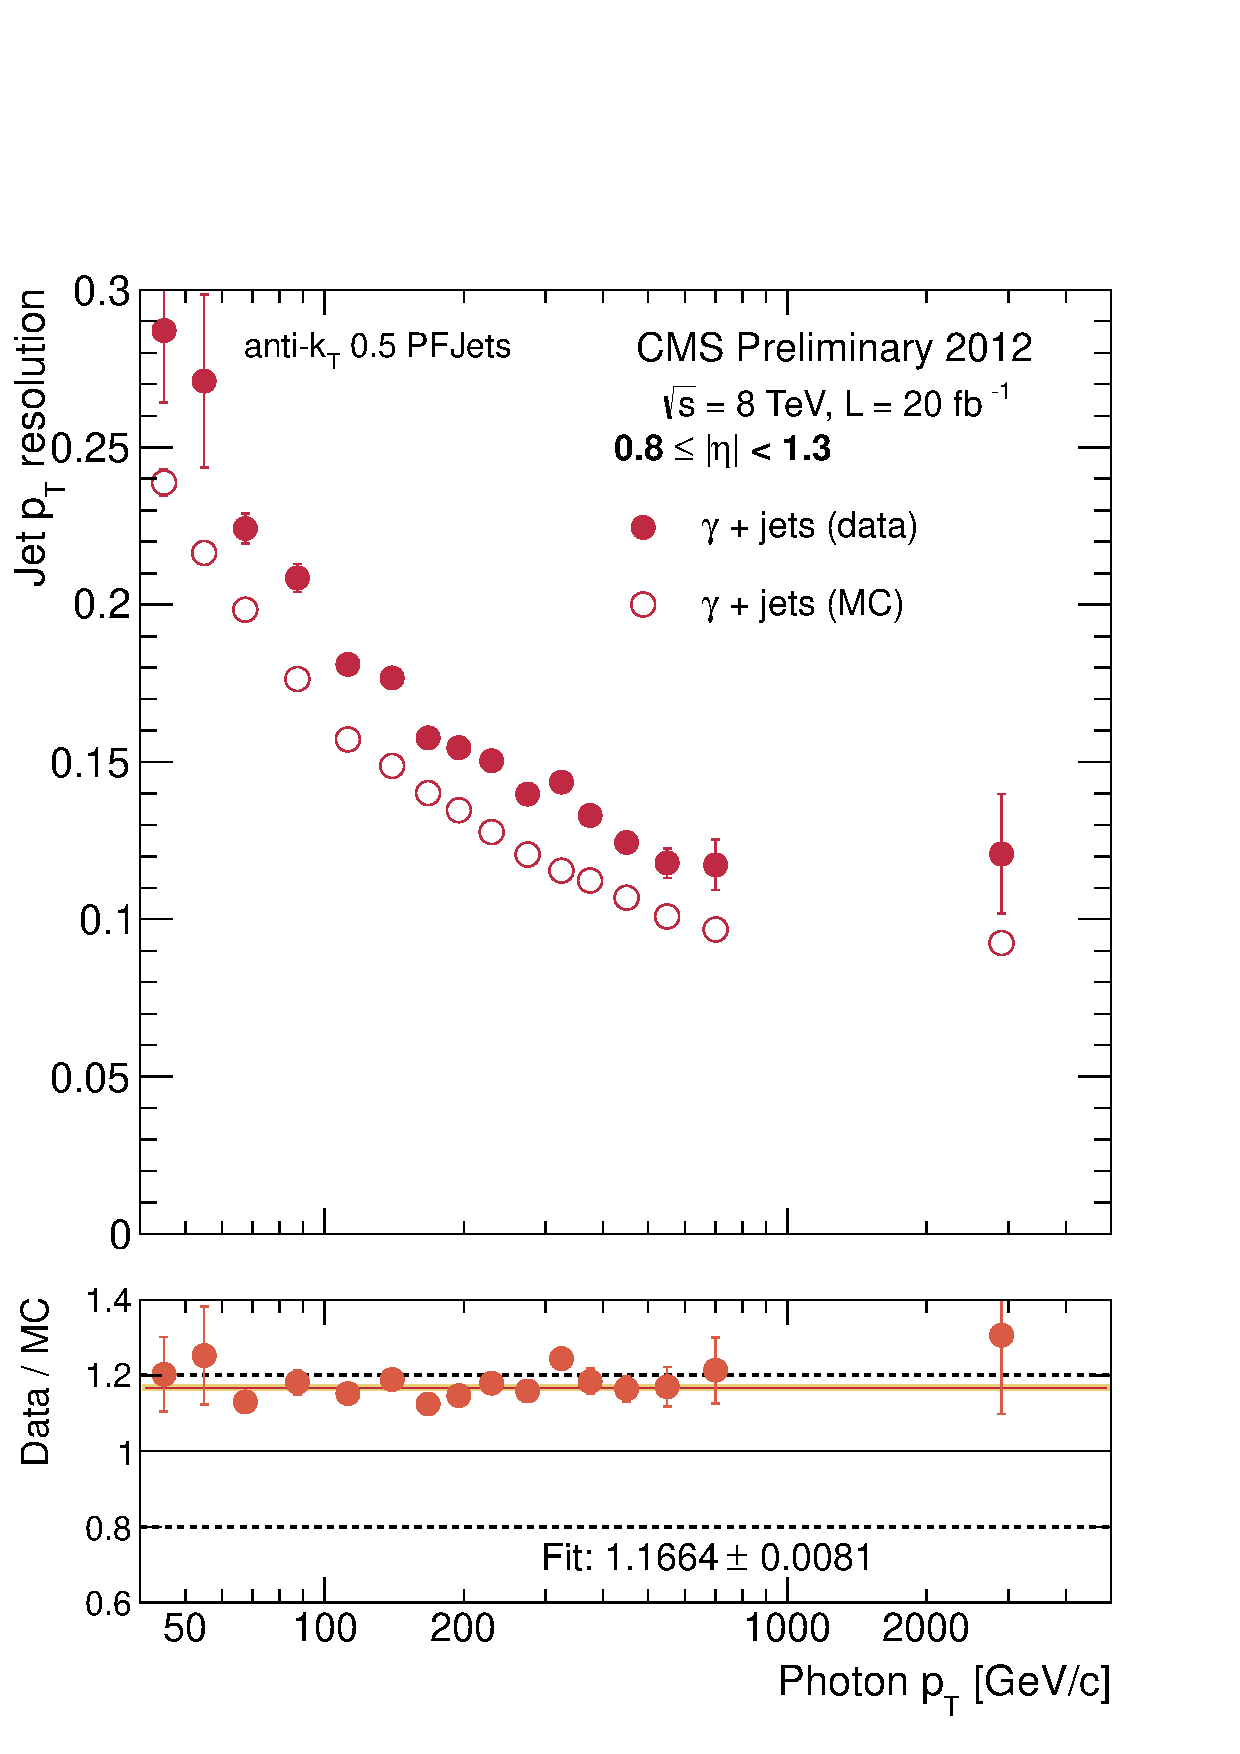
\includegraphics[width=0.45\textwidth]{chapitre4/figs/reso_balancing/resolution_eta0813_balancing.pdf}}
    \subcaptionbox{\label{fig:reso_bal_eta1319}}[0.45\textwidth]{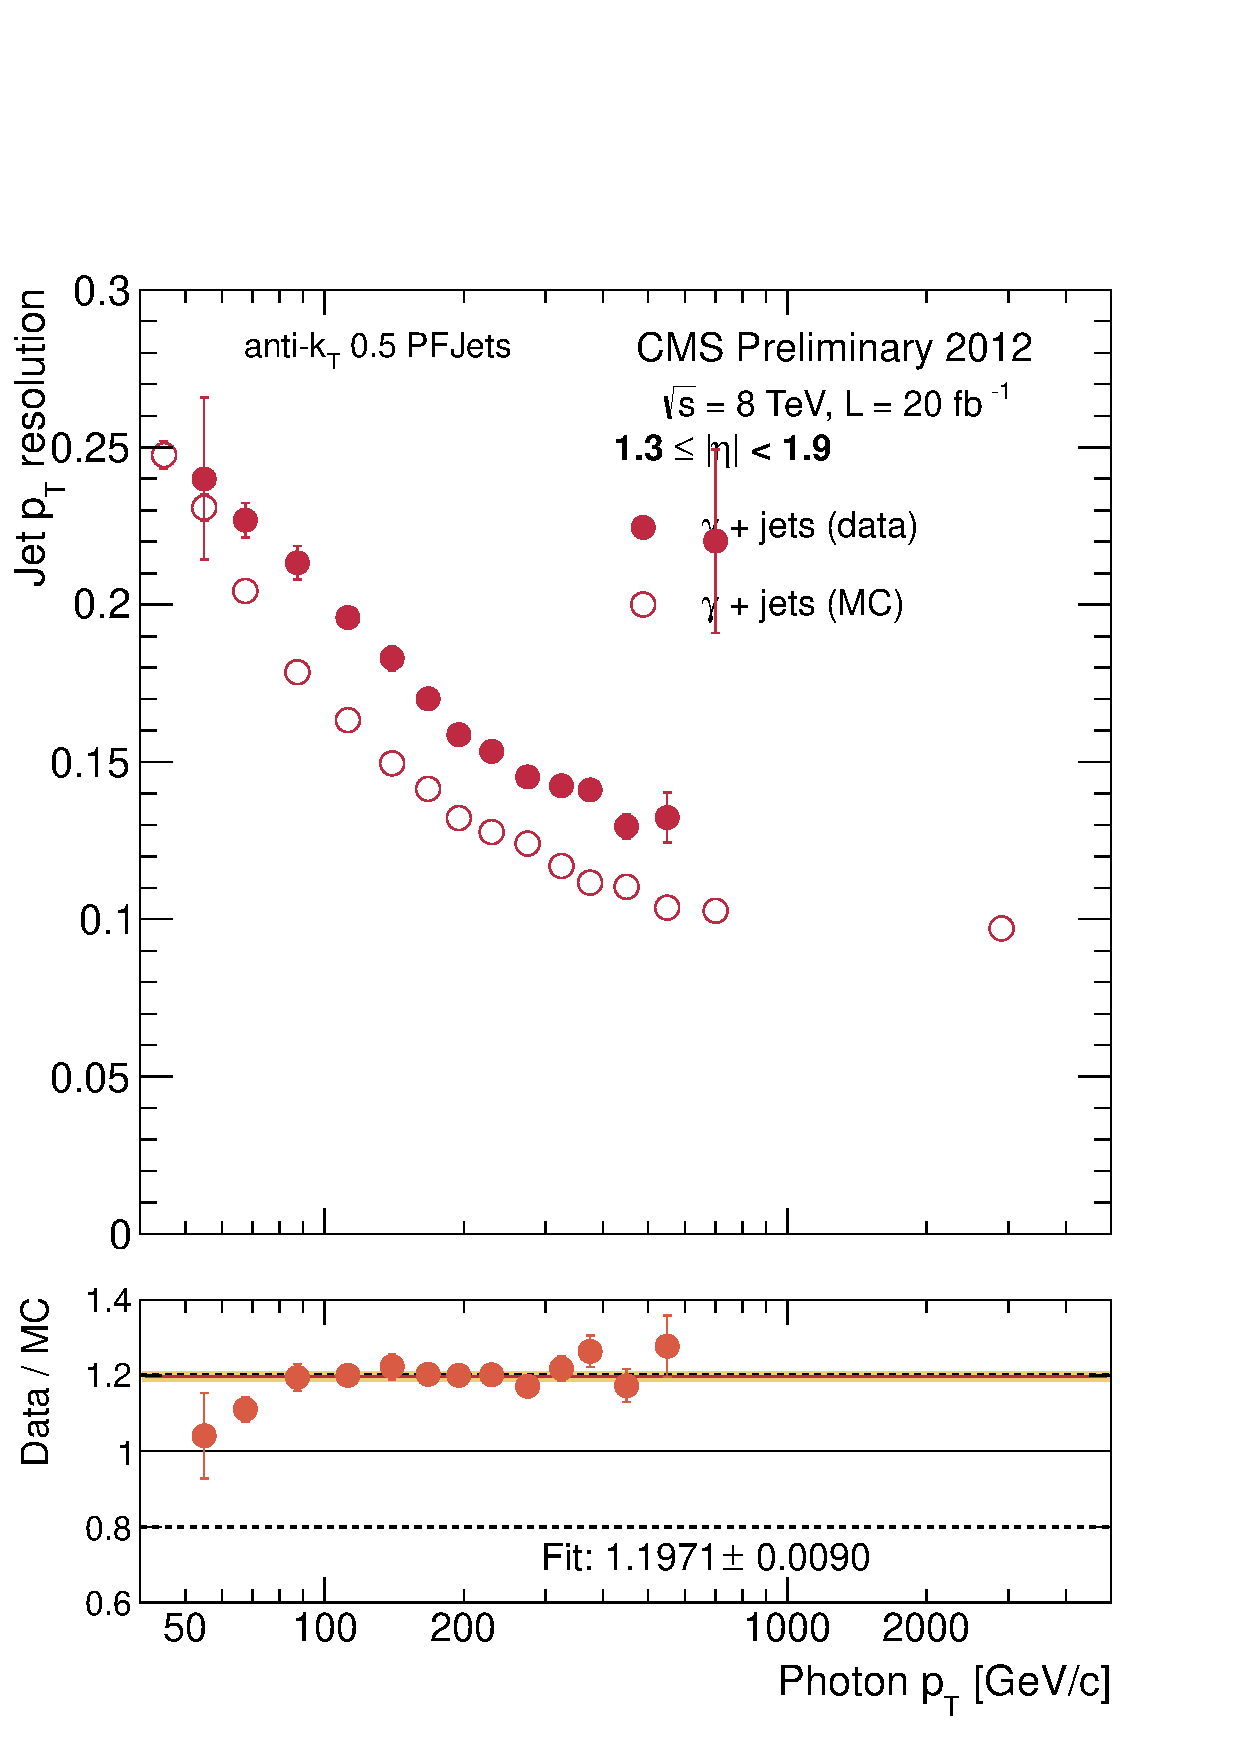
\includegraphics[width=0.45\textwidth]{chapitre4/figs/reso_balancing/resolution_eta1319_balancing.pdf}}\hfill
    \subcaptionbox{\label{fig:reso_bal_eta1925}}[0.45\textwidth]{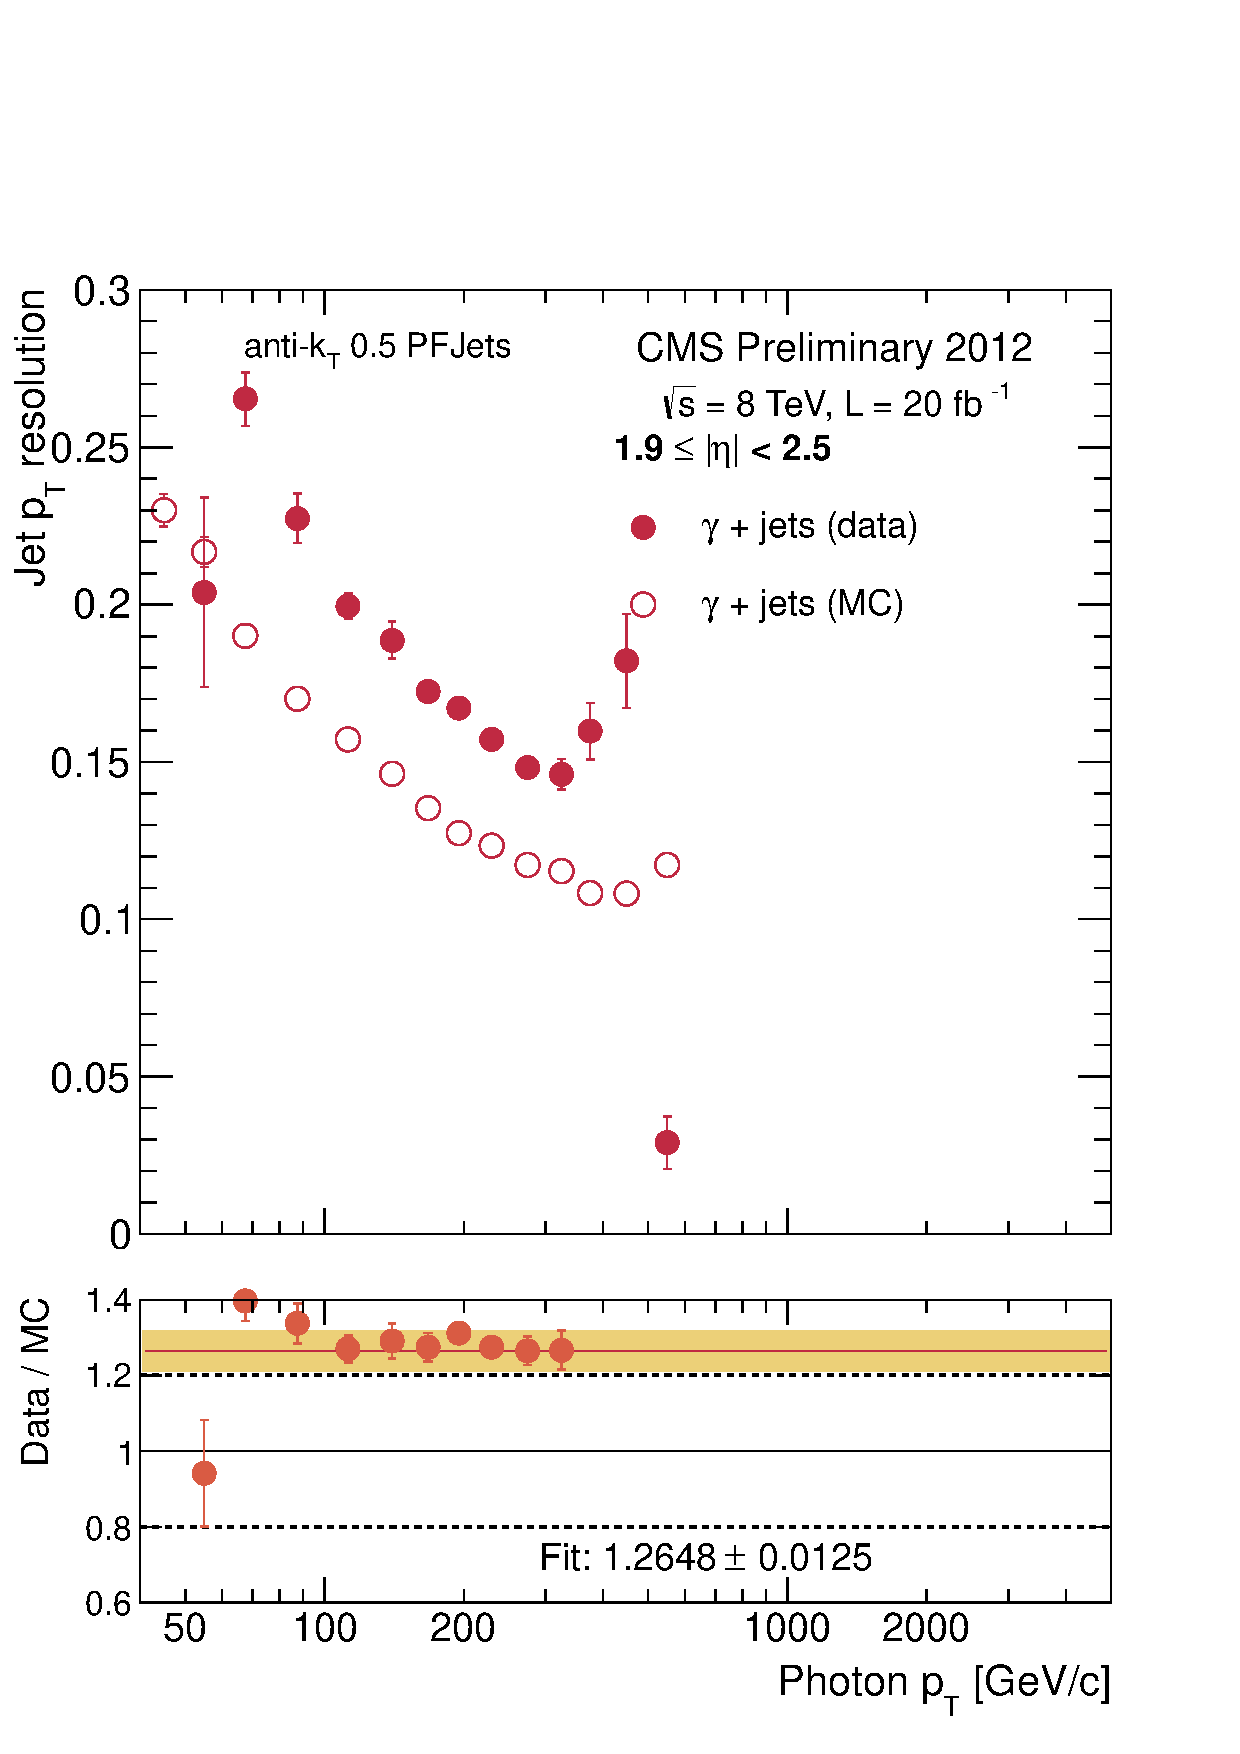
\includegraphics[width=0.45\textwidth]{chapitre4/figs/reso_balancing/resolution_eta1925_balancing.pdf}}
    \caption{Résolutions pour la méthode de la balance pour $\aeta < \num{0.8}$ (\subref{fig:reso_bal_eta008}), $\num{0.8} \leq \aeta < \num{1.3}$ (\subref{fig:reso_bal_eta0813}), $\num{1.3} \leq \aeta < \num{1.9}$ (\subref{fig:reso_bal_eta1319}), et $\num{1.9} \leq \aeta < \num{2.5}$ (\subref{fig:reso_bal_eta1925}). Le ratio entre les données et la simulation est présenté sous chaque distribution, accompagné d'une interpolation linéaire constante (ligne grise).}
    \label{fig:balancing_reso}
\end{figure}

\bigskip

On présente dans le \cref{tab:res_balancing} un résumé des ratios et des facteurs de correction extraient pour chaque classe en \aeta.

Le ratio est stable dans le tonneau ($\aeta < \num{2.1}$), avec un facteur de correction d'environ \SI{4}{\%}. Dans les bouchons, le ratio chute jusqu'à des facteurs de correction atteignant \SI{23}{\%}. Au delà de \SI{3.2}{\radian}, il n'y a plus de trajectographe, et la réponse devient très mauvaise.

\begin{table}[p!] \centering
 \begin{tabular}{@{}ccc@{}} \toprule
 Classe en \aeta & ratio & $f$ \\ \midrule
 \num{0} - \num{0.8} & \num{0.9659 \pm 0.0011} & \num{1.0353 \pm 0.0012}\\
 \num{0.8} - \num{1.3} & \num{0.9574 \pm 0.0013} & \num{1.0444 \pm 0.0014}\\
 \num{1.3} - \num{1.9} & \num{0.9580 \pm 0.0013} & \num{1.0439 \pm 0.0014}\\
 \num{1.9} - \num{2.5} & \num{0.9350 \pm 0.0019} & \num{1.0695 \pm 0.0022}\\
 \num{2.5} - \num{3} & \num{0.9093 \pm 0.0038} & \num{1.0997 \pm 0.0046}\\
 \num{3} - \num{3.2} & \num{0.8133 \pm 0.0120} & \num{1.2296 \pm 0.0182}\\
 \num{3.2} - \num{5.2} & \num{0.4286 \pm 0.0250} & \num{2.3333 \pm 0.1361}\\
 \bottomrule
 \end{tabular}
 \caption{Ratios et facteurs de correction pour différentes classes en \aeta obtenus grâce à la méthode de la balance, sans extrapolation.}
 \label{tab:res_balancing}
\end{table}

\begin{table}[p!] \centering
 \begin{tabular}{@{}ccc@{}} \toprule
 Classe en \aeta & ratio & $f$ \\ \midrule
 \num{0} - \num{0.8} & \num{0.9738 \pm 0.0007} & \num{1.0269 \pm 0.0007}\\
 \num{0.8} - \num{1.3} & \num{0.9656 \pm 0.0010} & \num{1.0356 \pm 0.0011}\\
 \num{1.3} - \num{1.9} & \num{0.9611 \pm 0.0013} & \num{1.0405 \pm 0.0014}\\
 \num{1.9} - \num{2.5} & \num{0.9435 \pm 0.0020} & \num{1.0599 \pm 0.0023}\\
 \num{2.5} - \num{3} & \num{0.9233 \pm 0.0048} & \num{1.0831 \pm 0.0056}\\
 \num{3} - \num{3.2} & \num{0.8442 \pm 0.0128} & \num{1.1845 \pm 0.0180}\\
 \num{3.2} - \num{5.2} & \num{0.3008 \pm 0.0051} & \num{3.3240 \pm 0.0567}\\
 \bottomrule
 \end{tabular}
 \caption{Ratios et facteurs de correction pour différentes classes en \aeta obtenus grâce à la méthode de la balance, avec extrapolation.}
 \label{tab:res_balancing_extrap}
\end{table}

\subsubsection{Méthode de la balance, avec extrapolation} \label{sec:res_balancing_extrap}

\begin{figure}[tbp]
    \centering
    \subcaptionbox{\label{fig:extrap_balancing}}[0.45\textwidth]{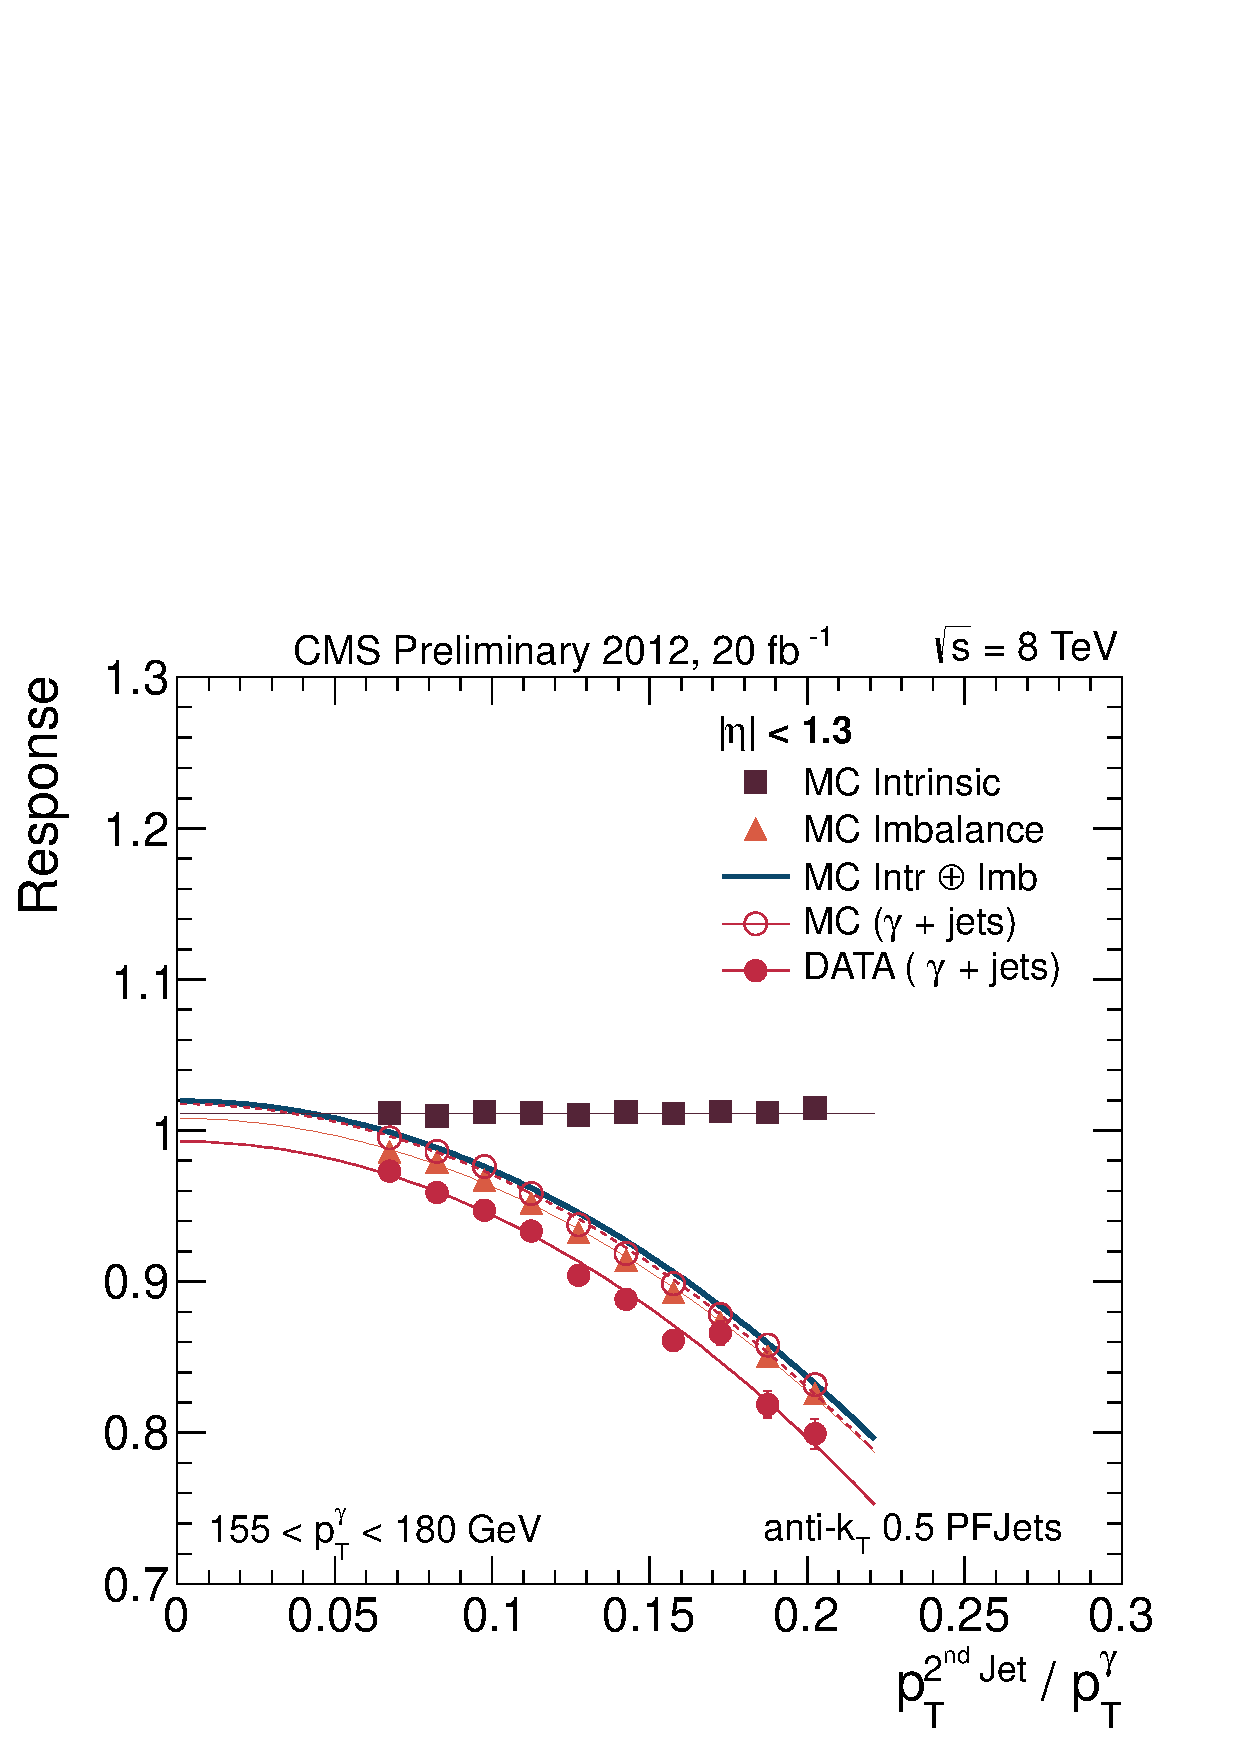
\includegraphics[width=0.45\textwidth]{chapitre4/figs/extrap/response_eta013_ptPhot_155_180.pdf}}\hfill
    \subcaptionbox{\label{fig:extrap_mpf}}[0.45\textwidth]{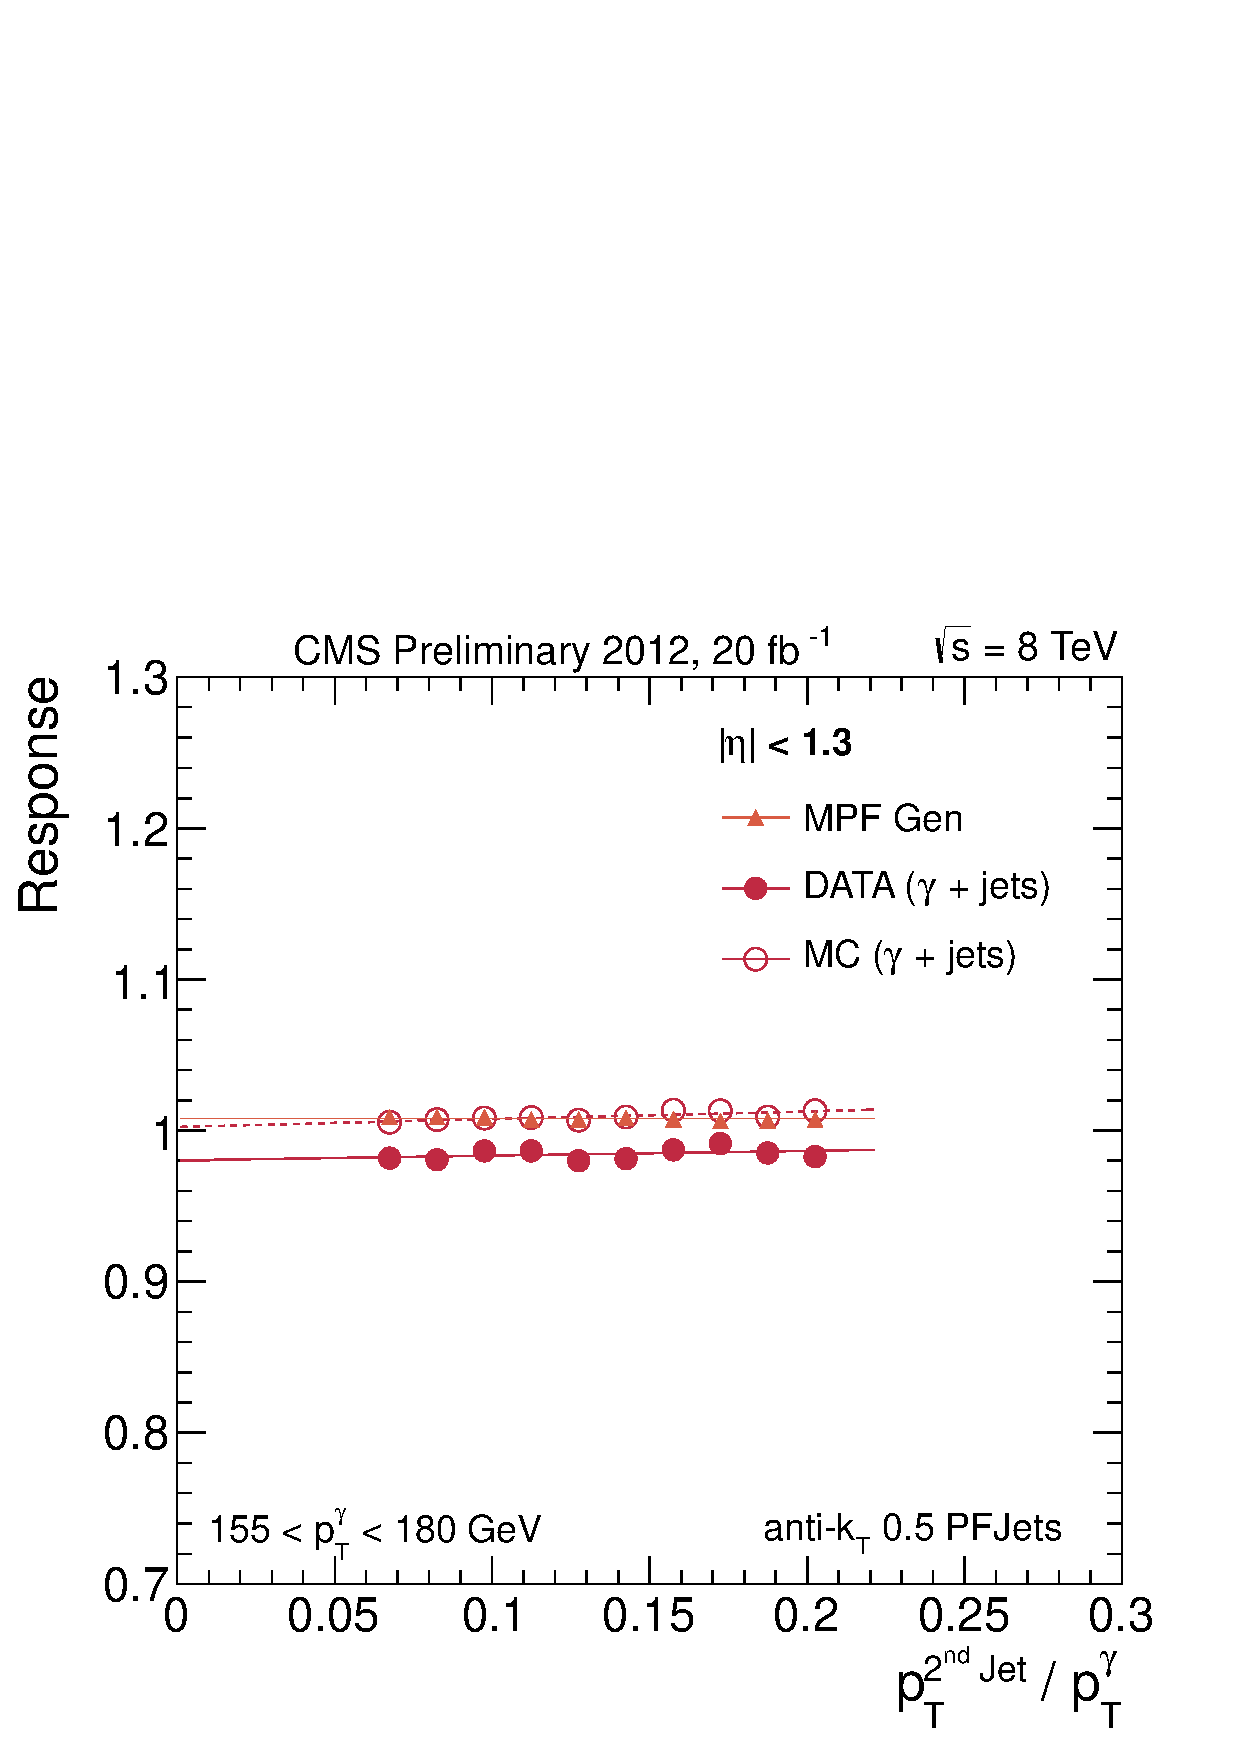
\includegraphics[width=0.45\textwidth]{chapitre4/figs/extrap/responseMPF_eta013_ptPhot_155_180.pdf}}
    \caption{Extrapolation de la réponse moyenne pour la méthode de la balance (\subref{fig:extrap_balancing}) et la méthode MPF (\subref{fig:extrap_mpf}). Pour la méthode de la balance, la réponse de la simulation (MC) a été séparée en deux parties, détaillées \cref{sec:res_balancing_extrap}.}
\end{figure}

On a vu précédemment que la méthode de la balance était sensible à la présence de jets additionnels dans l'événement. Afin de contrer cet effet, on extrapole la réponse moyenne à $\alpha \rightarrow 0$. On présente \cref{fig:extrap_balancing} un exemple d'extrapolation pour la méthode de la balance, pour $155 \leq p_T^\gamma < \SI{180}{\GeV}$ et $\aeta < \num{1.3}$, et \cref{fig:extrap_mpf} pour la méthode MPF. On constate une très nette dépendance de la réponse moyenne en fonction de $\alpha$ pour la méthode de la balance, dépendance quasi inexistante pour la méthode MPF.

Pour la méthode de la balance, on sépare la réponse de la simulation en deux parties. On a
\begin{align*}
  R_m &= \frac{\ptfjet}{\ptg} = \underbrace{ \frac{\ptfjet}{p_T^{\text{\ordinalnum{1} jet généré}}} }_{\text{intrinsèque}} \; \times \; \underbrace{ \frac{p_T^{\text{\ordinalnum{1} jet généré}}}{\ptg} }_{\text{déséquilibre}}
\end{align*}

%\afterpage{\clearpage}

La partie intrinsèque n'est pas dépendante de la présence de jets additionnels, d'où l'allure plate \cref{fig:extrap_balancing}. Elle est uniquement sensible aux problèmes de calibrations des divers détecteurs, problèmes résolus à l'aide des corrections de niveau 1, 2 et 3. C'est ainsi qu'on obtient une réponse intrinsèque très proche de l'unité. La deuxième partie correspond au déséquilibre entre le photon et le premier jet de l'événement, et dépend fortement de $\alpha$.

\begin{figure}[p!]
    \centering
    \subcaptionbox{\label{fig:bal_extrap_eta008}}[0.45\textwidth]{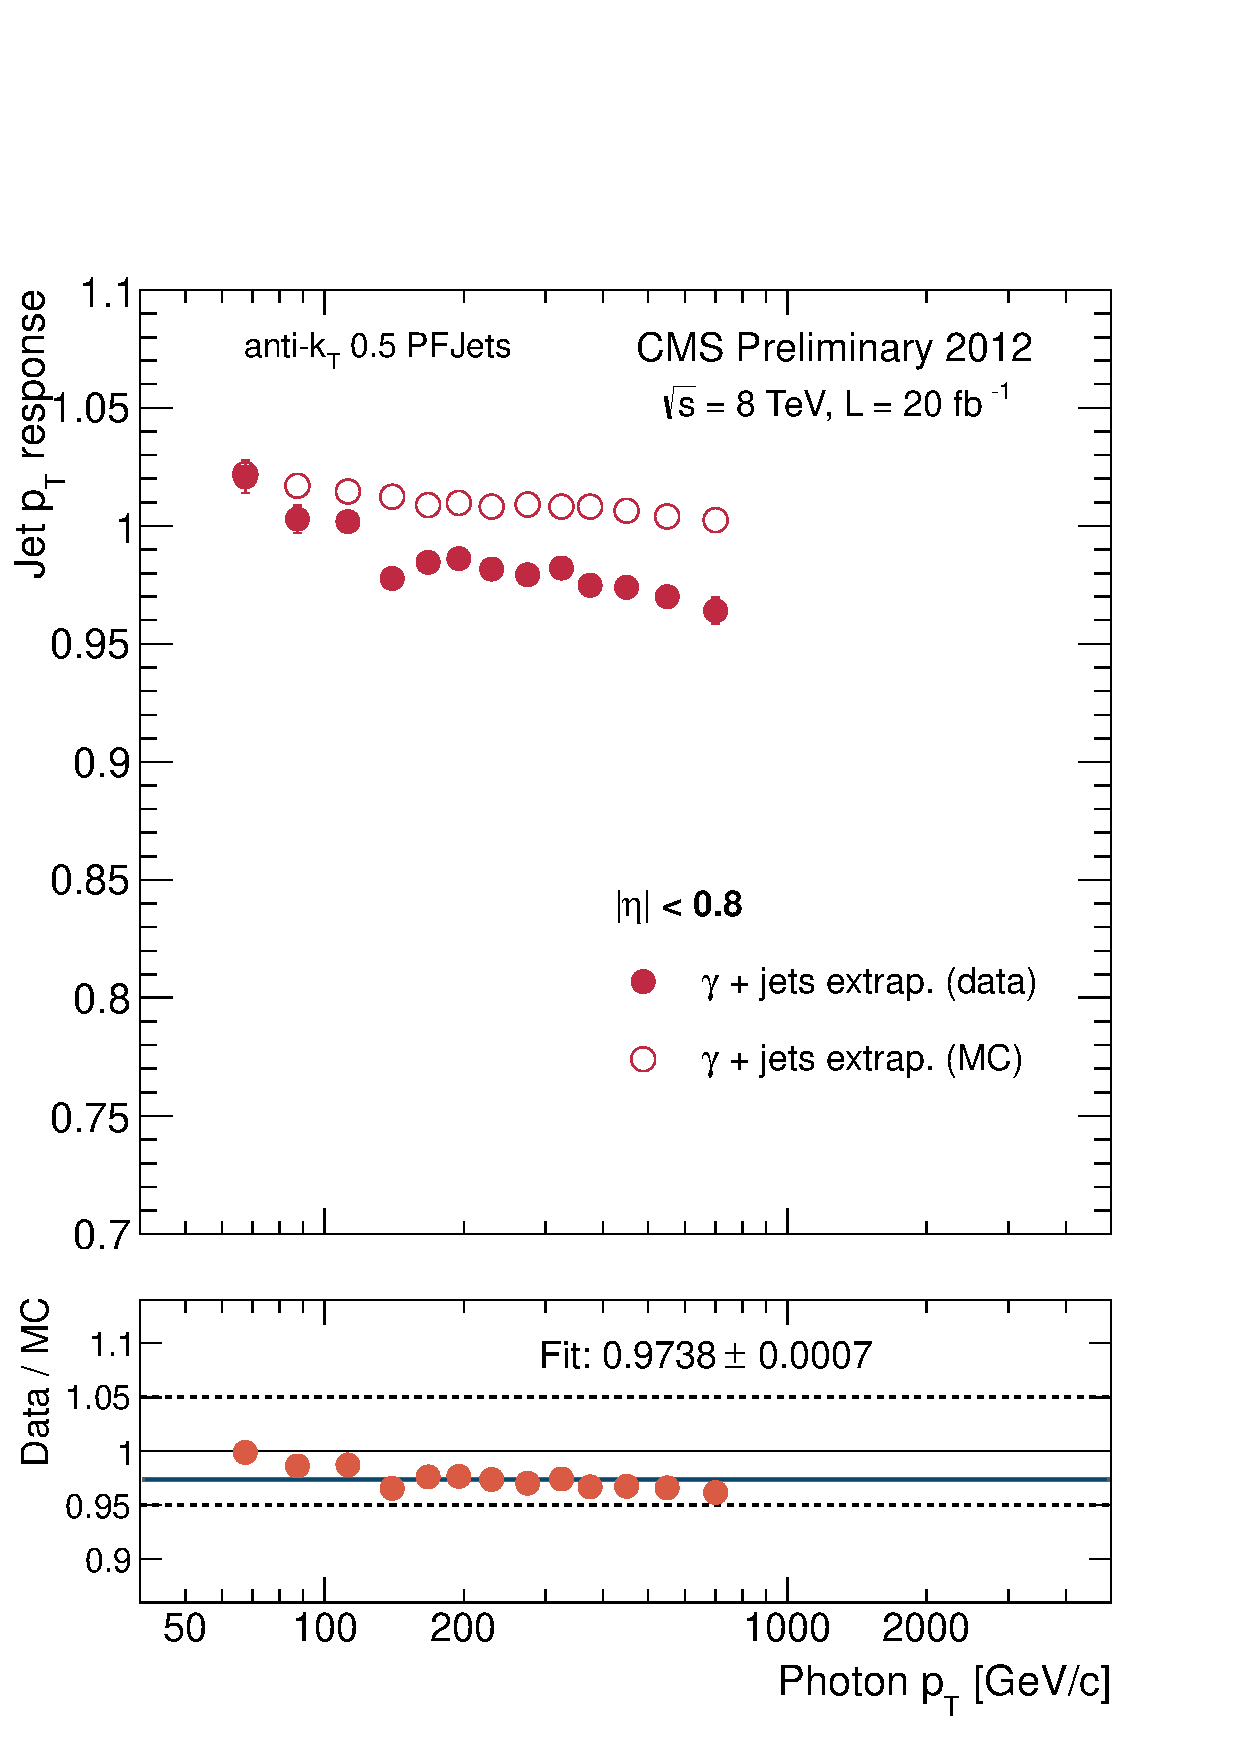
\includegraphics[width=0.45\textwidth]{chapitre4/figs/resp_balancing_extrap/response_eta008_balancing_extrap.pdf}}\hfill
    \subcaptionbox{\label{fig:bal_extrap_eta0813}}[0.45\textwidth]{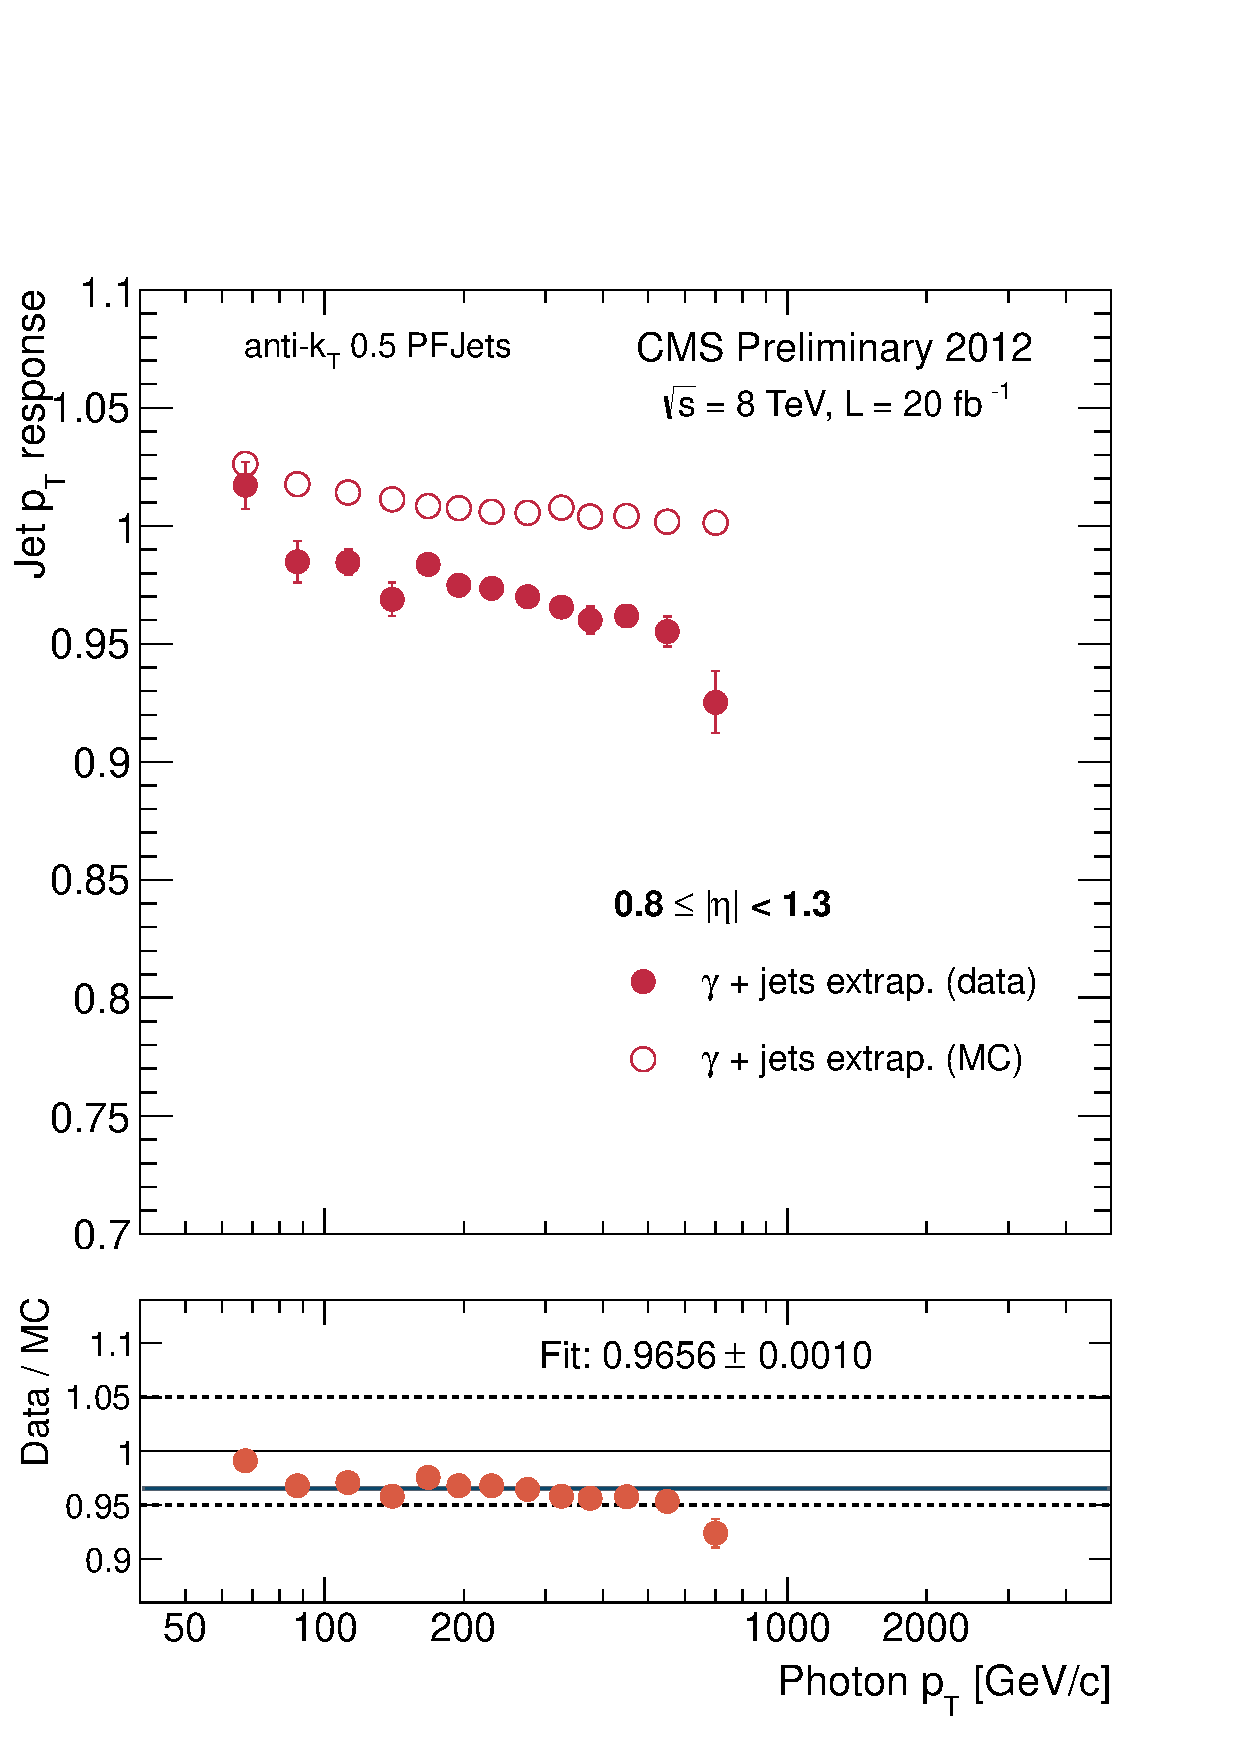
\includegraphics[width=0.45\textwidth]{chapitre4/figs/resp_balancing_extrap/response_eta0813_balancing_extrap.pdf}}
    \subcaptionbox{\label{fig:bal_extrap_eta1319}}[0.45\textwidth]{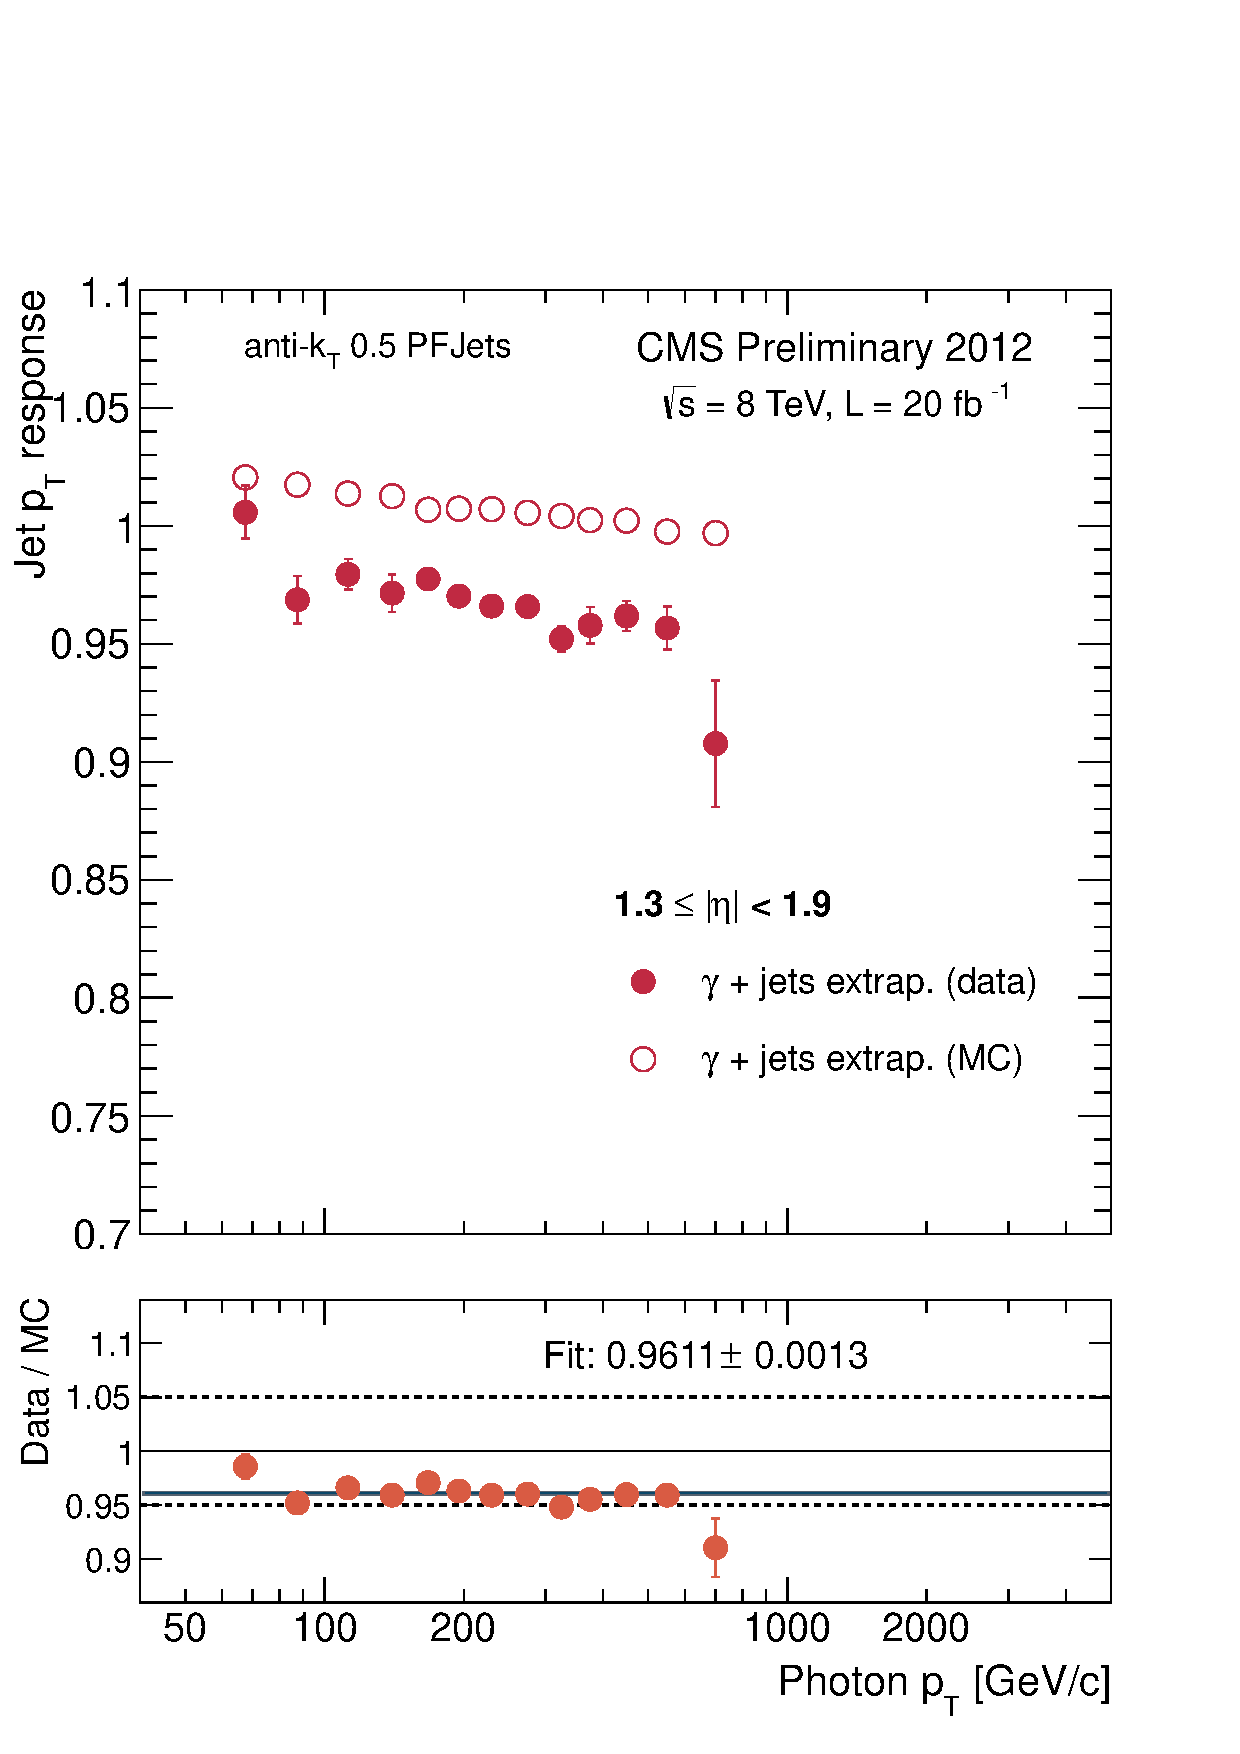
\includegraphics[width=0.45\textwidth]{chapitre4/figs/resp_balancing_extrap/response_eta1319_balancing_extrap.pdf}}\hfill
    \subcaptionbox{\label{fig:bal_extrap_eta1925}}[0.45\textwidth]{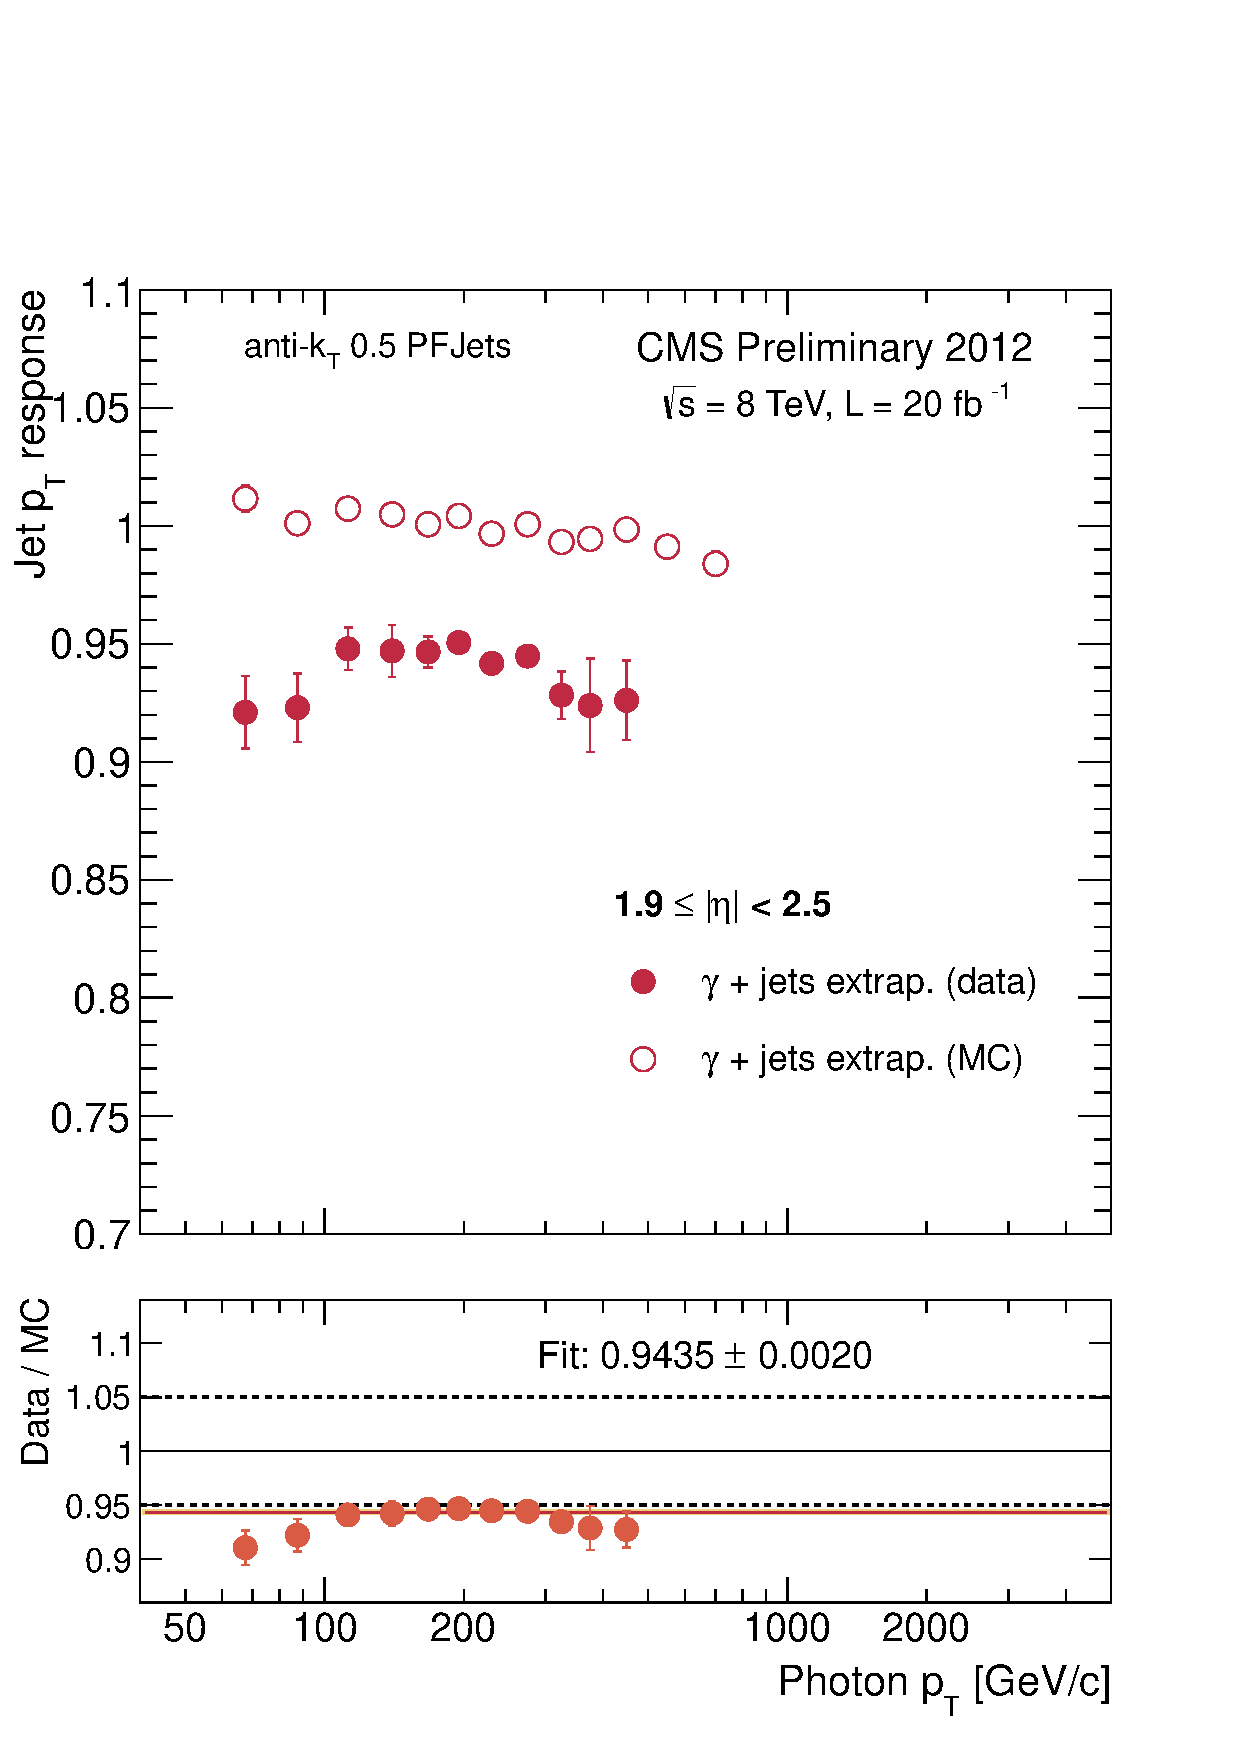
\includegraphics[width=0.45\textwidth]{chapitre4/figs/resp_balancing_extrap/response_eta1925_balancing_extrap.pdf}}
    \caption{Réponses moyennes pour la méthode de la balance, avec extrapolation, pour $\aeta < \num{0.8}$ (\subref{fig:bal_extrap_eta008}), $\num{0.8} \leq \aeta < \num{1.3}$ (\subref{fig:bal_extrap_eta0813}), $\num{1.3} \leq \aeta < \num{1.9}$ (\subref{fig:bal_extrap_eta1319}), et $\num{1.9} \leq \aeta < \num{2.5}$ (\subref{fig:bal_extrap_eta1925}). Le ratio entre les données et la simulation est présenté sous chaque distribution, accompagné d'une interpolation linéaire constante (ligne grise).}
    \label{fig:balancing_extrap_resp}
\end{figure}

\begin{figure}[p!]
    \centering
    \subcaptionbox{\label{fig:reso_bal_extrap_eta008}}[0.45\textwidth]{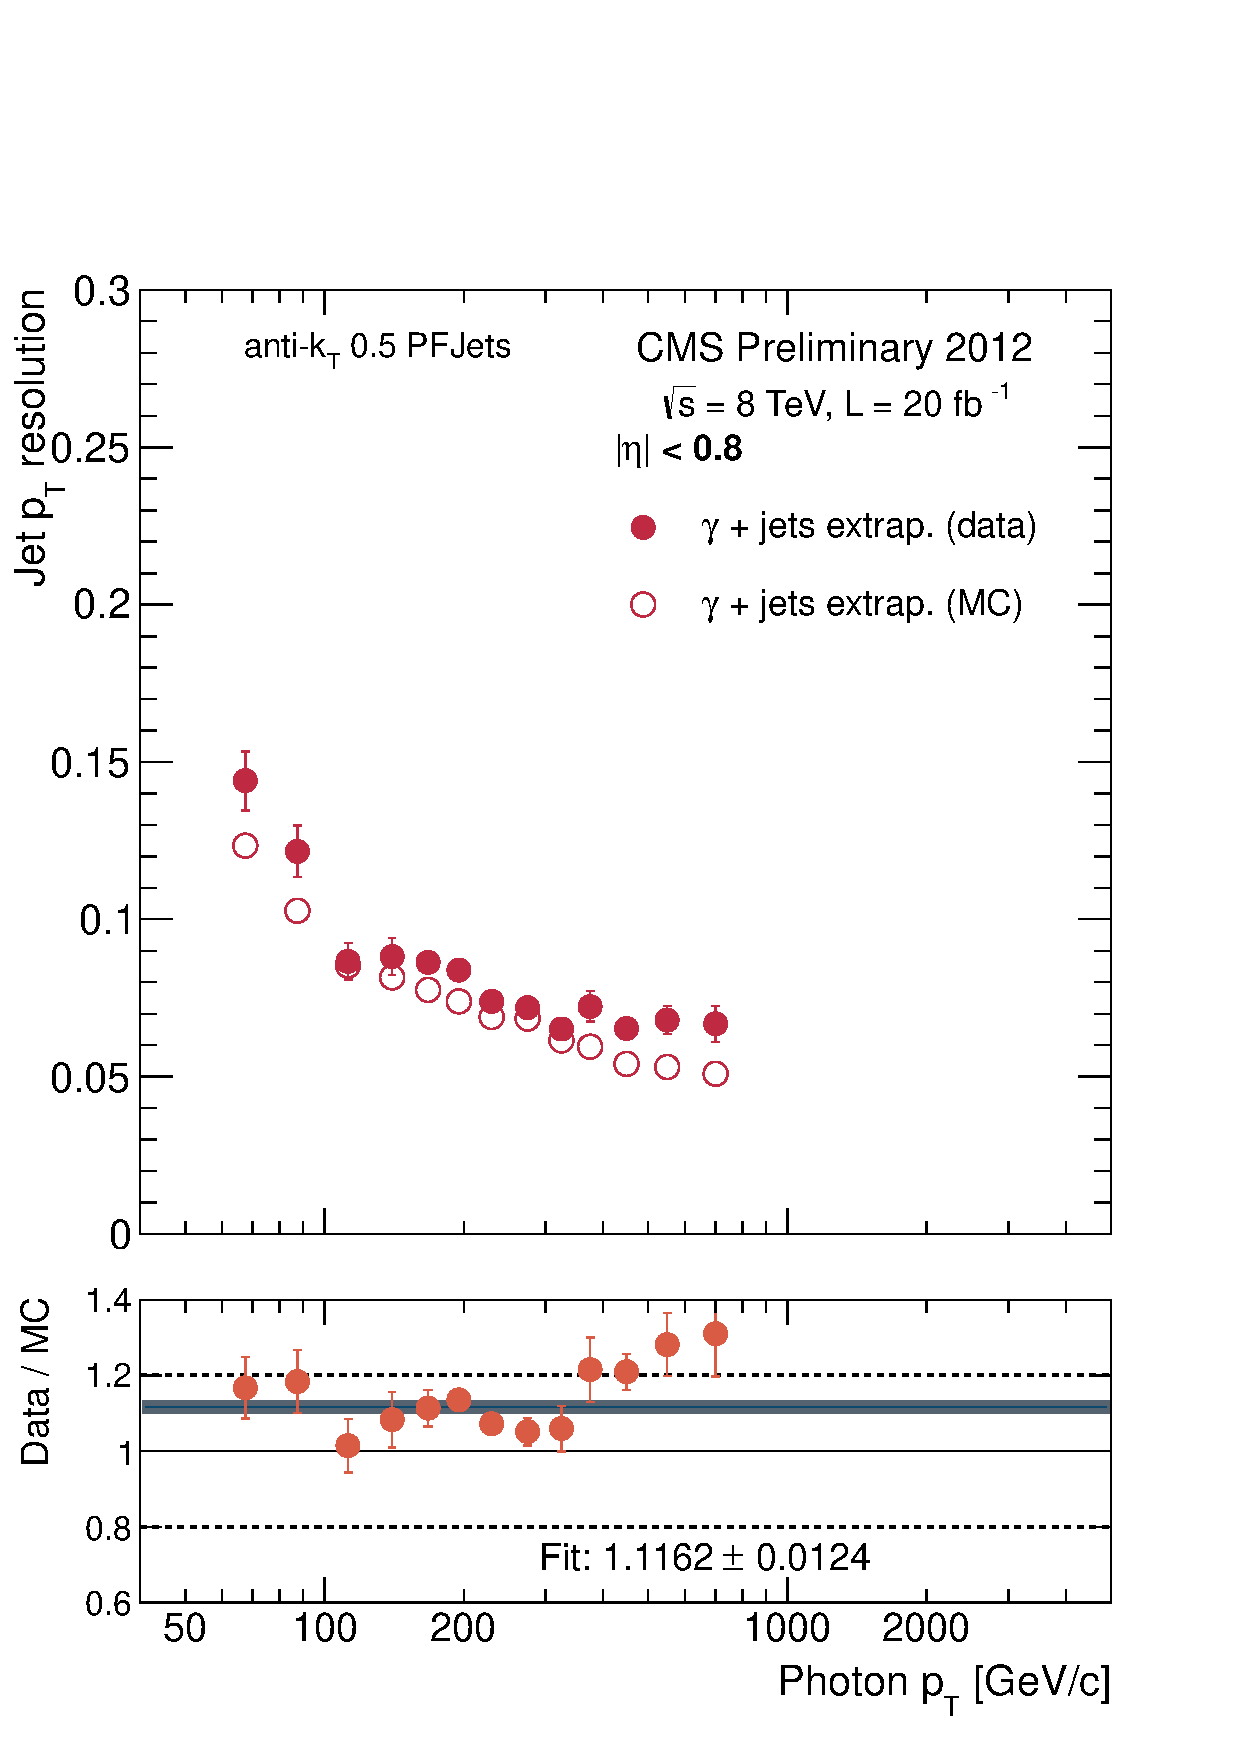
\includegraphics[width=0.45\textwidth]{chapitre4/figs/reso_balancing_extrap/resolution_eta008_balancing_extrap.pdf}}\hfill
    \subcaptionbox{\label{fig:reso_bal_extrap_eta0813}}[0.45\textwidth]{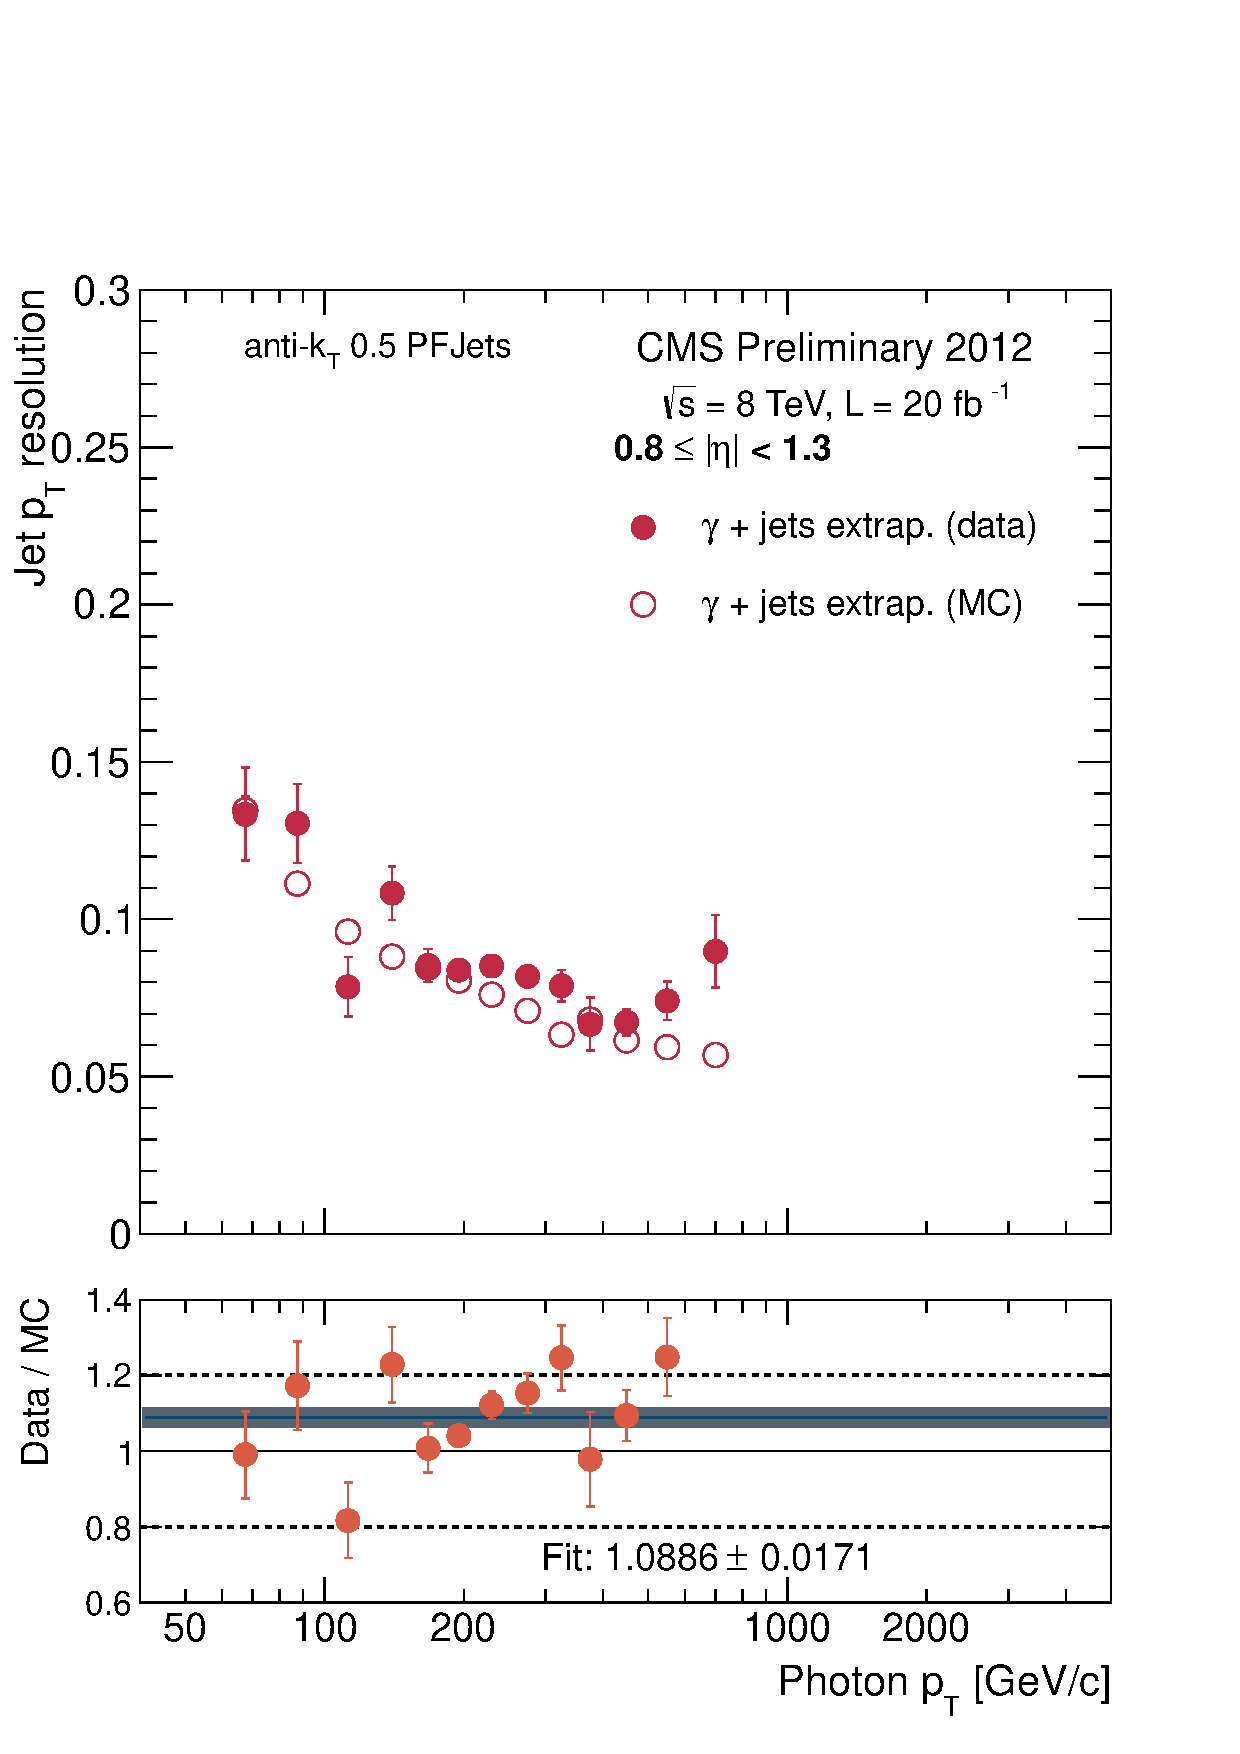
\includegraphics[width=0.45\textwidth]{chapitre4/figs/reso_balancing_extrap/resolution_eta0813_balancing_extrap.pdf}}
    \subcaptionbox{\label{fig:reso_bal_extrap_eta1319}}[0.45\textwidth]{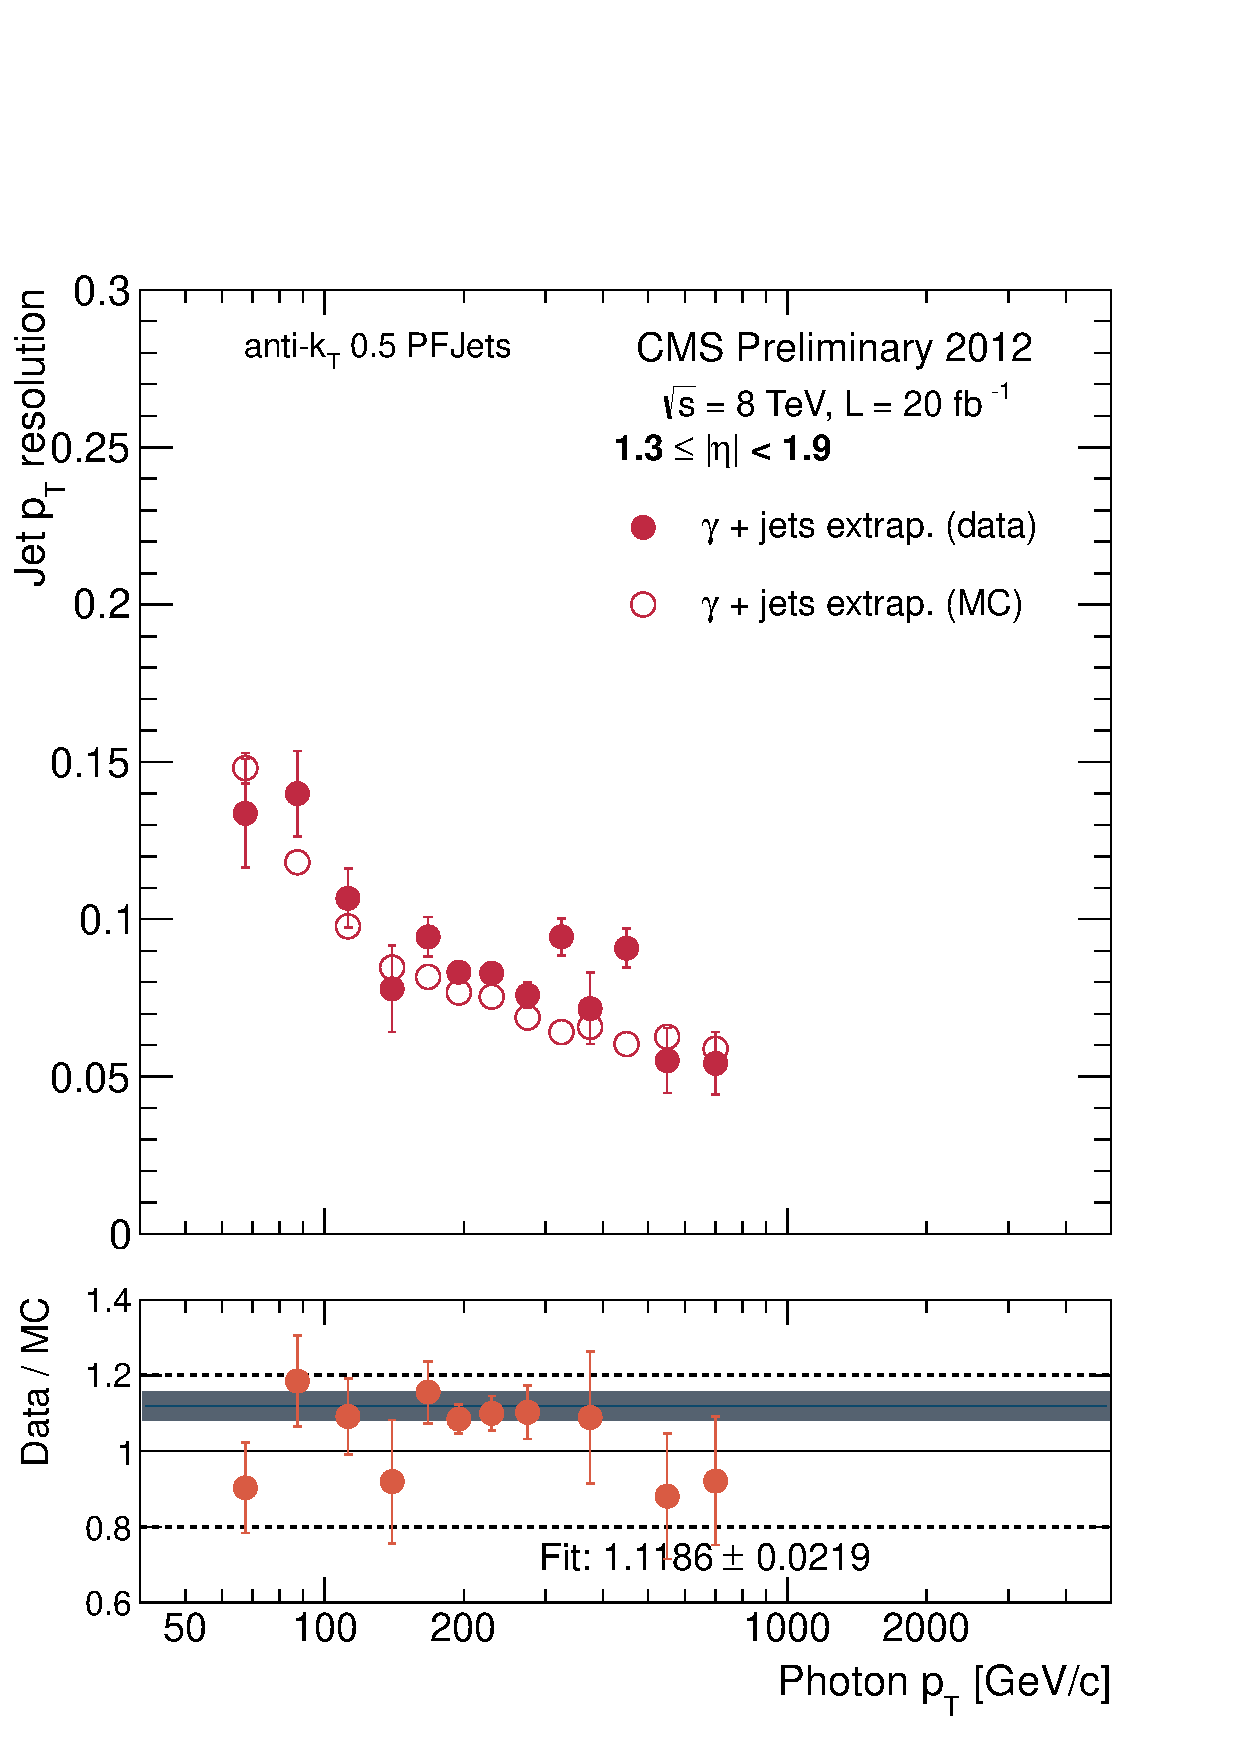
\includegraphics[width=0.45\textwidth]{chapitre4/figs/reso_balancing_extrap/resolution_eta1319_balancing_extrap.pdf}}\hfill
    \subcaptionbox{\label{fig:reso_bal_extrap_eta1925}}[0.45\textwidth]{\includegraphics[width=0.45\textwidth]{chapitre4/figs/reso_balancing_extrap/resolution_eta1925_balancing_extrap.pdf}}
    \caption{Résolutions pour la méthode de la balance, avec extrapolation, pour $\aeta < \num{0.8}$ (\subref{fig:reso_bal_extrap_eta008}), $\num{0.8} \leq \aeta < \num{1.3}$ (\subref{fig:reso_bal_extrap_eta0813}), $\num{1.3} \leq \aeta < \num{1.9}$ (\subref{fig:reso_bal_extrap_eta1319}), et $\num{1.9} \leq \aeta < \num{2.5}$ (\subref{fig:reso_bal_extrap_eta1925}). Le ratio entre les données et la simulation est présenté sous chaque distribution, accompagné d'une interpolation linéaire constante (ligne grise).}
    \label{fig:balancing_extrap_reso}
\end{figure}

On utilise comme réponse moyenne la valeur de l'interpolation pour $\alpha = 0$, et on reproduit la même procédure que section précédente. À haut \pt et haut \aeta, la statistique n'est parfois pas suffisante pour réaliser l'extrapolation. Dans ce cas, le point est simplement ignoré et n'apparait pas dans la distribution des réponses.

On présente \cref{fig:balancing_extrap_resp} les distributions des réponses moyennes après extrapolation pour différentes classes en \aeta, et \cref{fig:balancing_extrap_reso} les résolutions associées. Les facteurs de correction sont récapitulés dans le \cref{tab:res_balancing_extrap}. On constate une légère amélioration des ratios pour toutes les classes en \aeta, sauf la dernière, où la statistique n'est pas suffisante pour effectuer une extrapolation sensée.

\subsubsection{Méthode MPF}

On présente les distributions des réponses moyennes obtenues avec la méthode MPF \cref{fig:mpf_resp}, et les résolutions associées \cref{fig:mpf_reso}. Un récapitulatif des résultats peut être trouvé dans le \cref{tab:res_mpf}.

\begin{table}[h!] \centering
 \begin{tabular}{@{}ccc@{}} \toprule
 Classe en \aeta & ratio & $f$ \\ \midrule
 \num{0} - \num{0.8} & \num{0.9748 \pm 0.0009} & \num{1.0258 \pm 0.0010} \\
 \num{0.8} - \num{1.3} & \num{0.9673 \pm 0.0011} & \num{1.0338 \pm 0.0012} \\
 \num{1.3} - \num{1.9} & \num{0.9649 \pm 0.0012} & \num{1.0364 \pm 0.0013} \\
 \num{1.9} - \num{2.5} & \num{0.9472 \pm 0.0014} & \num{1.0557 \pm 0.0016} \\
 \num{2.5} - \num{3} & \num{0.9270 \pm 0.0026} & \num{1.0788 \pm 0.0030} \\
 \num{3} - \num{3.2} & \num{0.8598 \pm 0.0097} & \num{1.1631 \pm 0.0131} \\
 \num{3.2} - \num{5.2} & \num{0.9191 \pm 0.0103} & \num{1.0881 \pm 0.0122} \\
 \bottomrule
 \end{tabular}
 \caption{Ratios et facteurs de correction pour différentes classes en \aeta obtenus grâce à la méthode MPF.}
 \label{tab:res_mpf}
\end{table}

\begin{figure}[p!]
    \centering
    \subcaptionbox{\label{fig:mpf_eta008}}[0.45\textwidth]{\includegraphics[width=0.45\textwidth]{chapitre4/figs/resp_mpf/response_eta008_mpf.pdf}}\hfill
    \subcaptionbox{\label{fig:mpf_eta0813}}[0.45\textwidth]{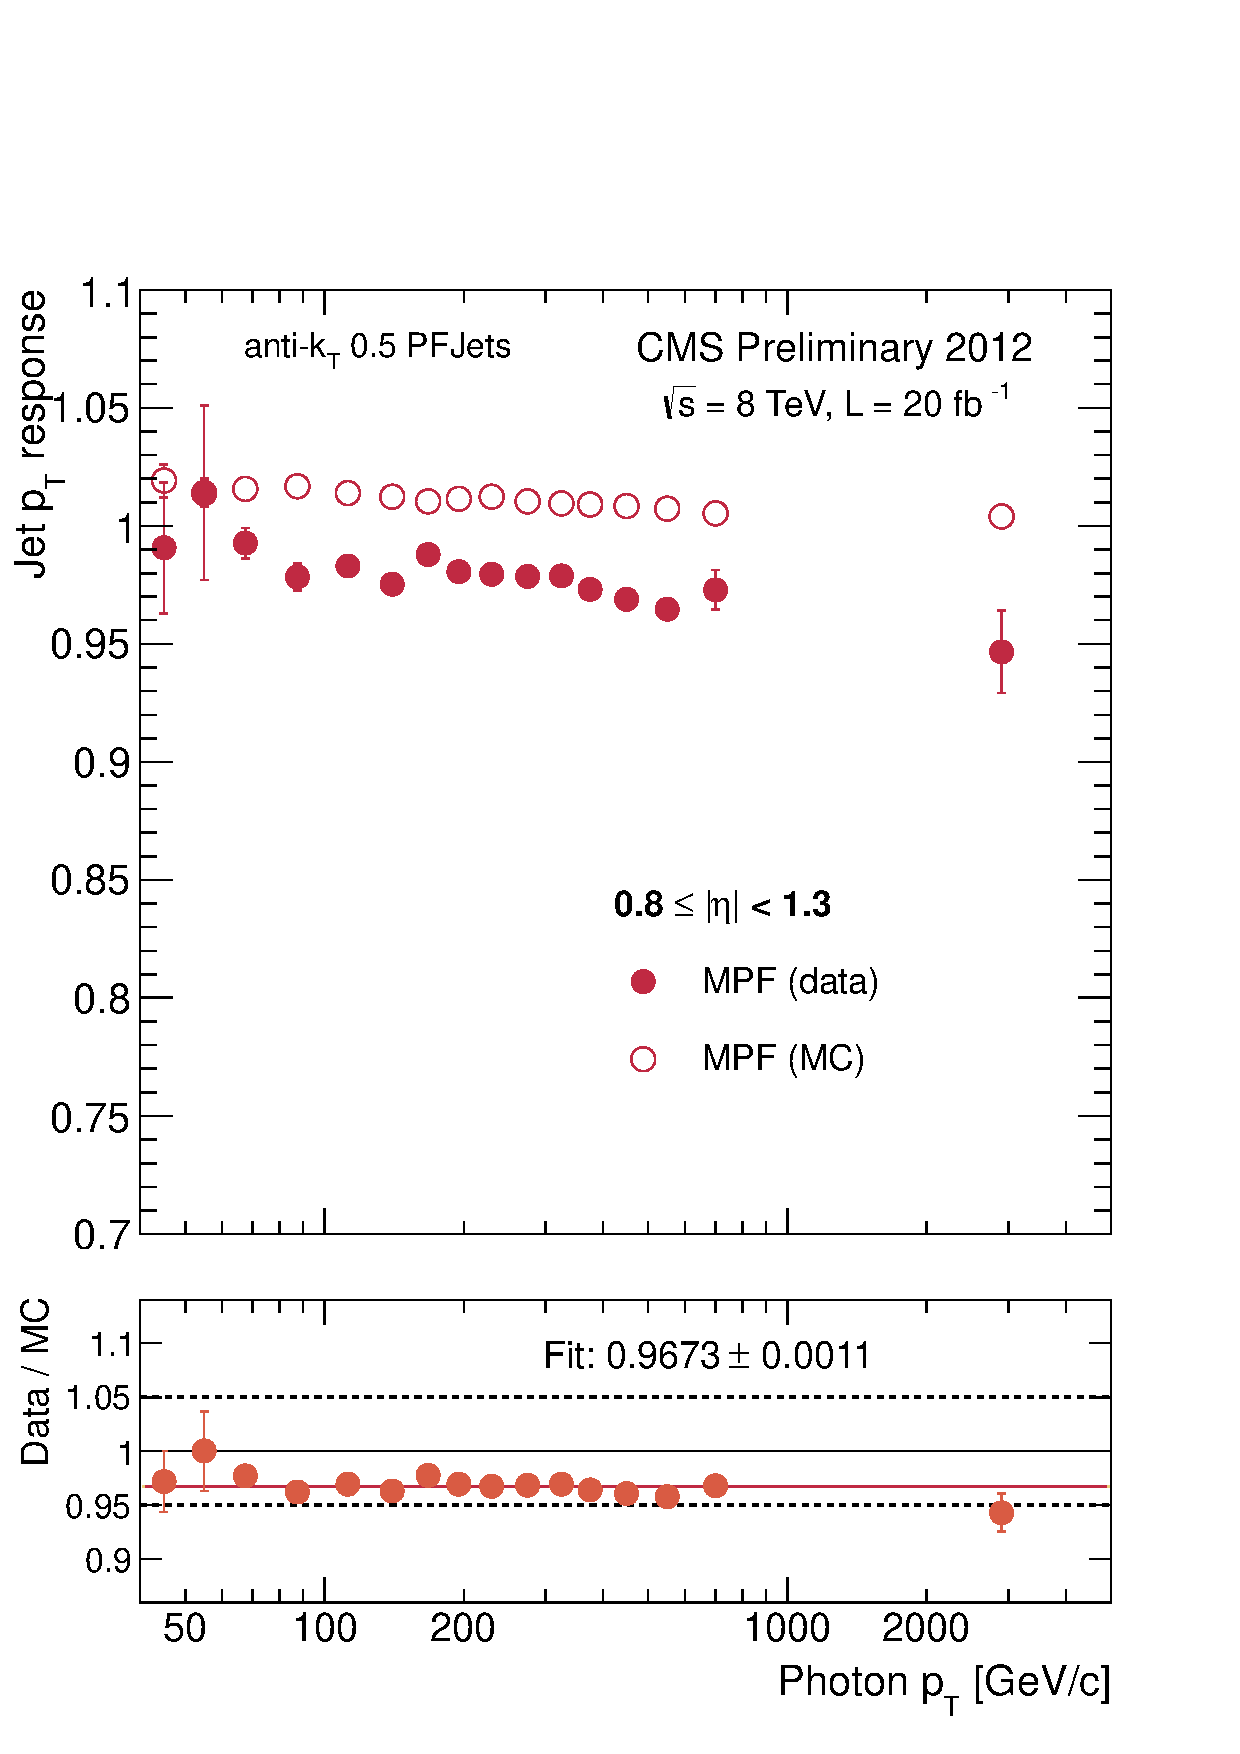
\includegraphics[width=0.45\textwidth]{chapitre4/figs/resp_mpf/response_eta0813_mpf.pdf}}
    \subcaptionbox{\label{fig:mpf_eta1319}}[0.45\textwidth]{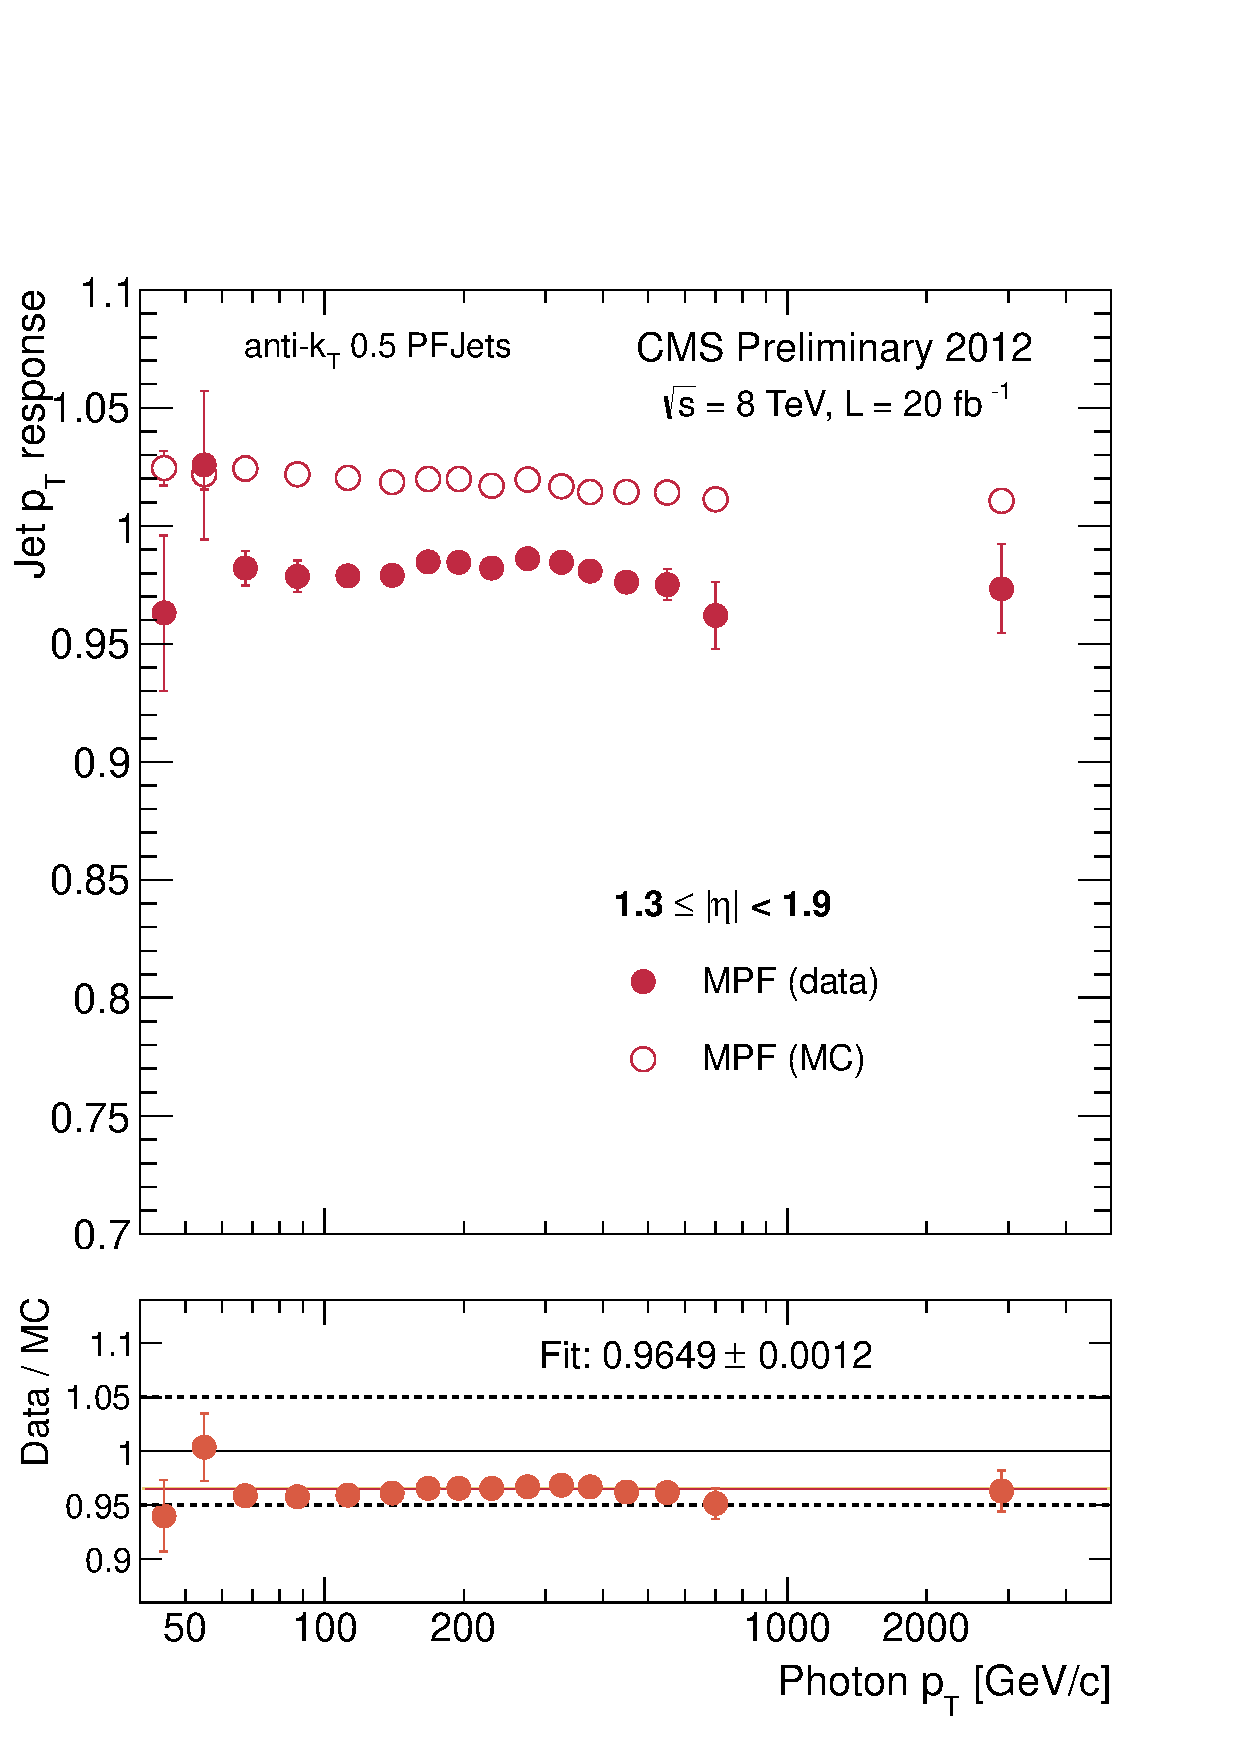
\includegraphics[width=0.45\textwidth]{chapitre4/figs/resp_mpf/response_eta1319_mpf.pdf}}\hfill
    \subcaptionbox{\label{fig:mpf_eta1925}}[0.45\textwidth]{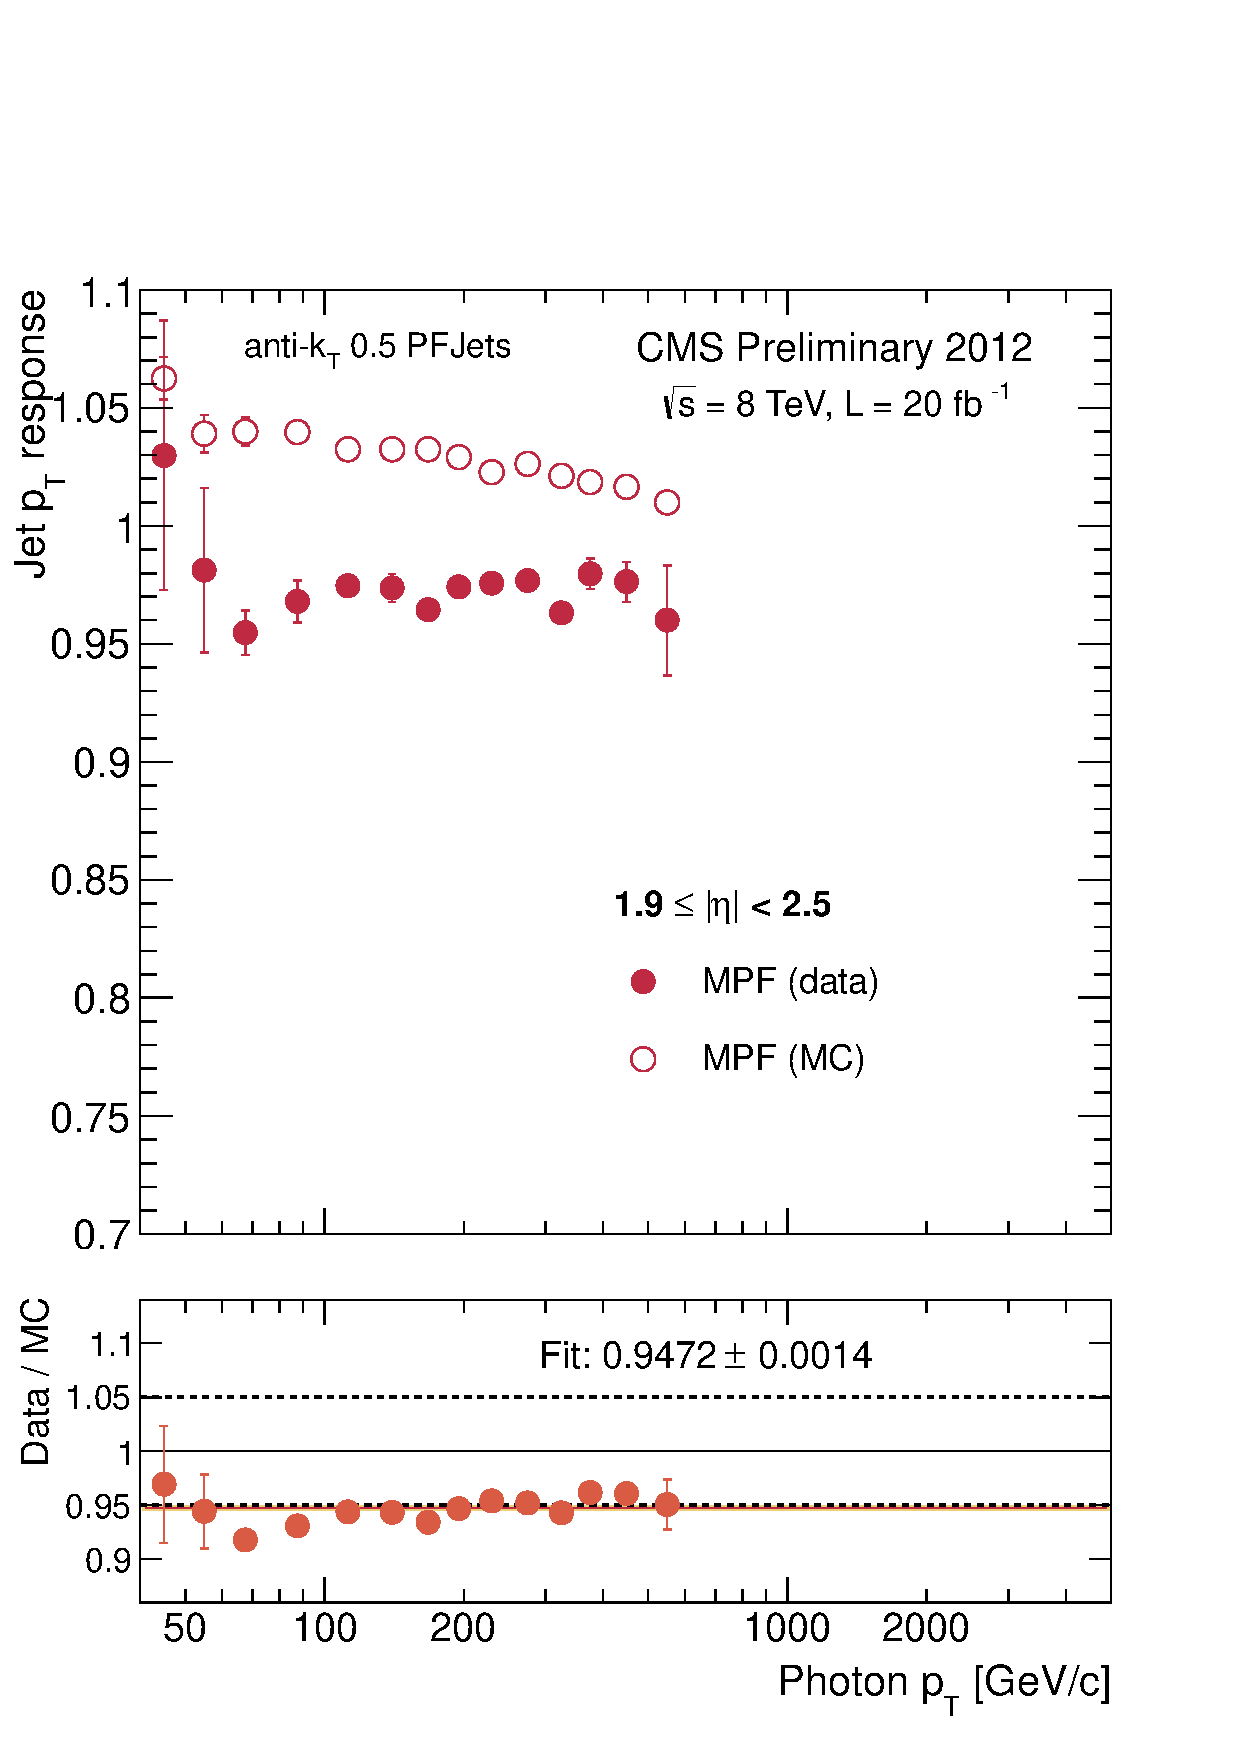
\includegraphics[width=0.45\textwidth]{chapitre4/figs/resp_mpf/response_eta1925_mpf.pdf}}
    \caption{Réponses moyennes pour la méthode MPF, sans extrapolation, pour $\aeta < \num{0.8}$ (\subref{fig:mpf_eta008}), $\num{0.8} \leq \aeta < \num{1.3}$ (\subref{fig:mpf_eta0813}), $\num{1.3} \leq \aeta < \num{1.9}$ (\subref{fig:mpf_eta1319}), et $\num{1.9} \leq \aeta < \num{2.5}$ (\subref{fig:mpf_eta1925}). Le ratio entre les données et la simulation est présenté sous chaque distribution, accompagné d'une interpolation linéaire constante (ligne grise)}
    \label{fig:mpf_resp}
\end{figure}

\begin{figure}[p!]
    \centering
    \subcaptionbox{\label{fig:reso_mpf_eta008}}[0.45\textwidth]{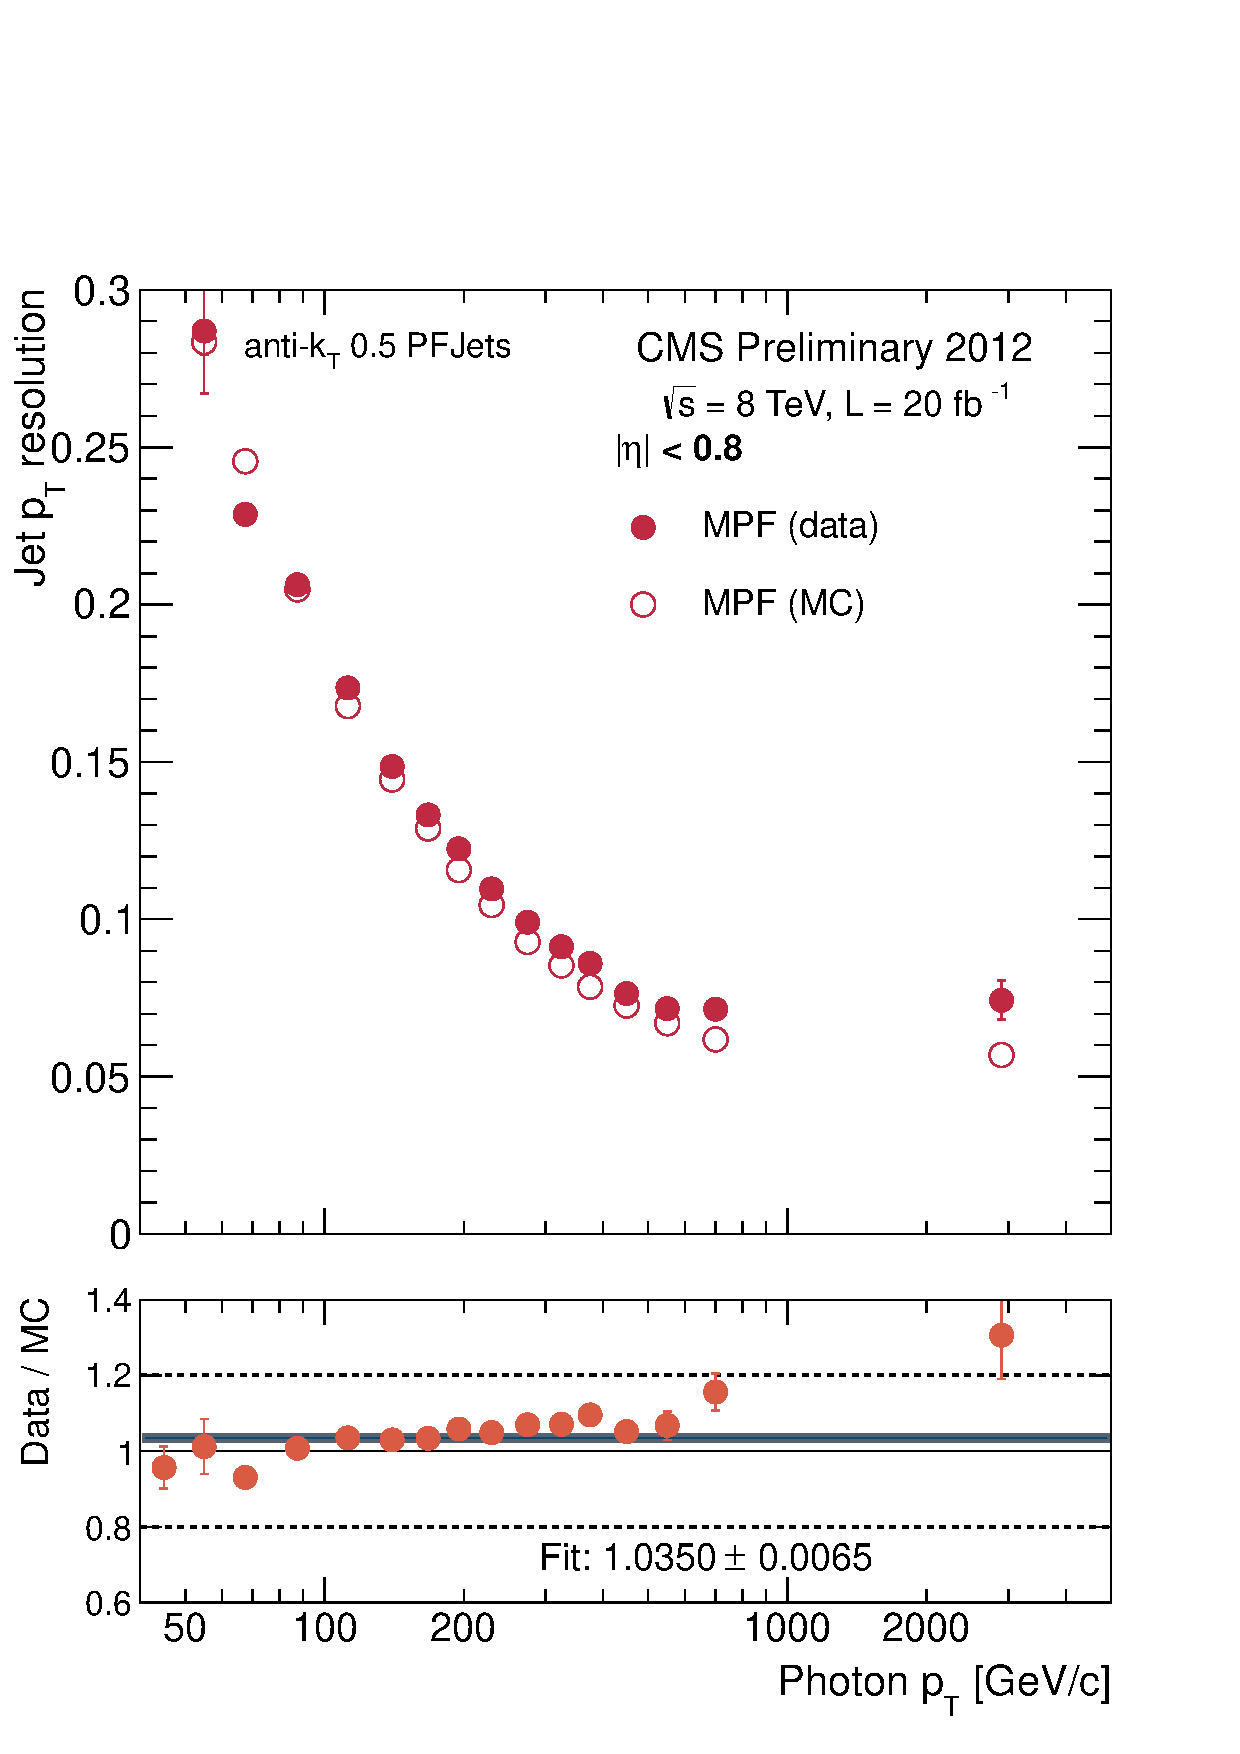
\includegraphics[width=0.45\textwidth]{chapitre4/figs/reso_mpf/resolution_eta008_mpf.pdf}}\hfill
    \subcaptionbox{\label{fig:reso_mpf_eta0813}}[0.45\textwidth]{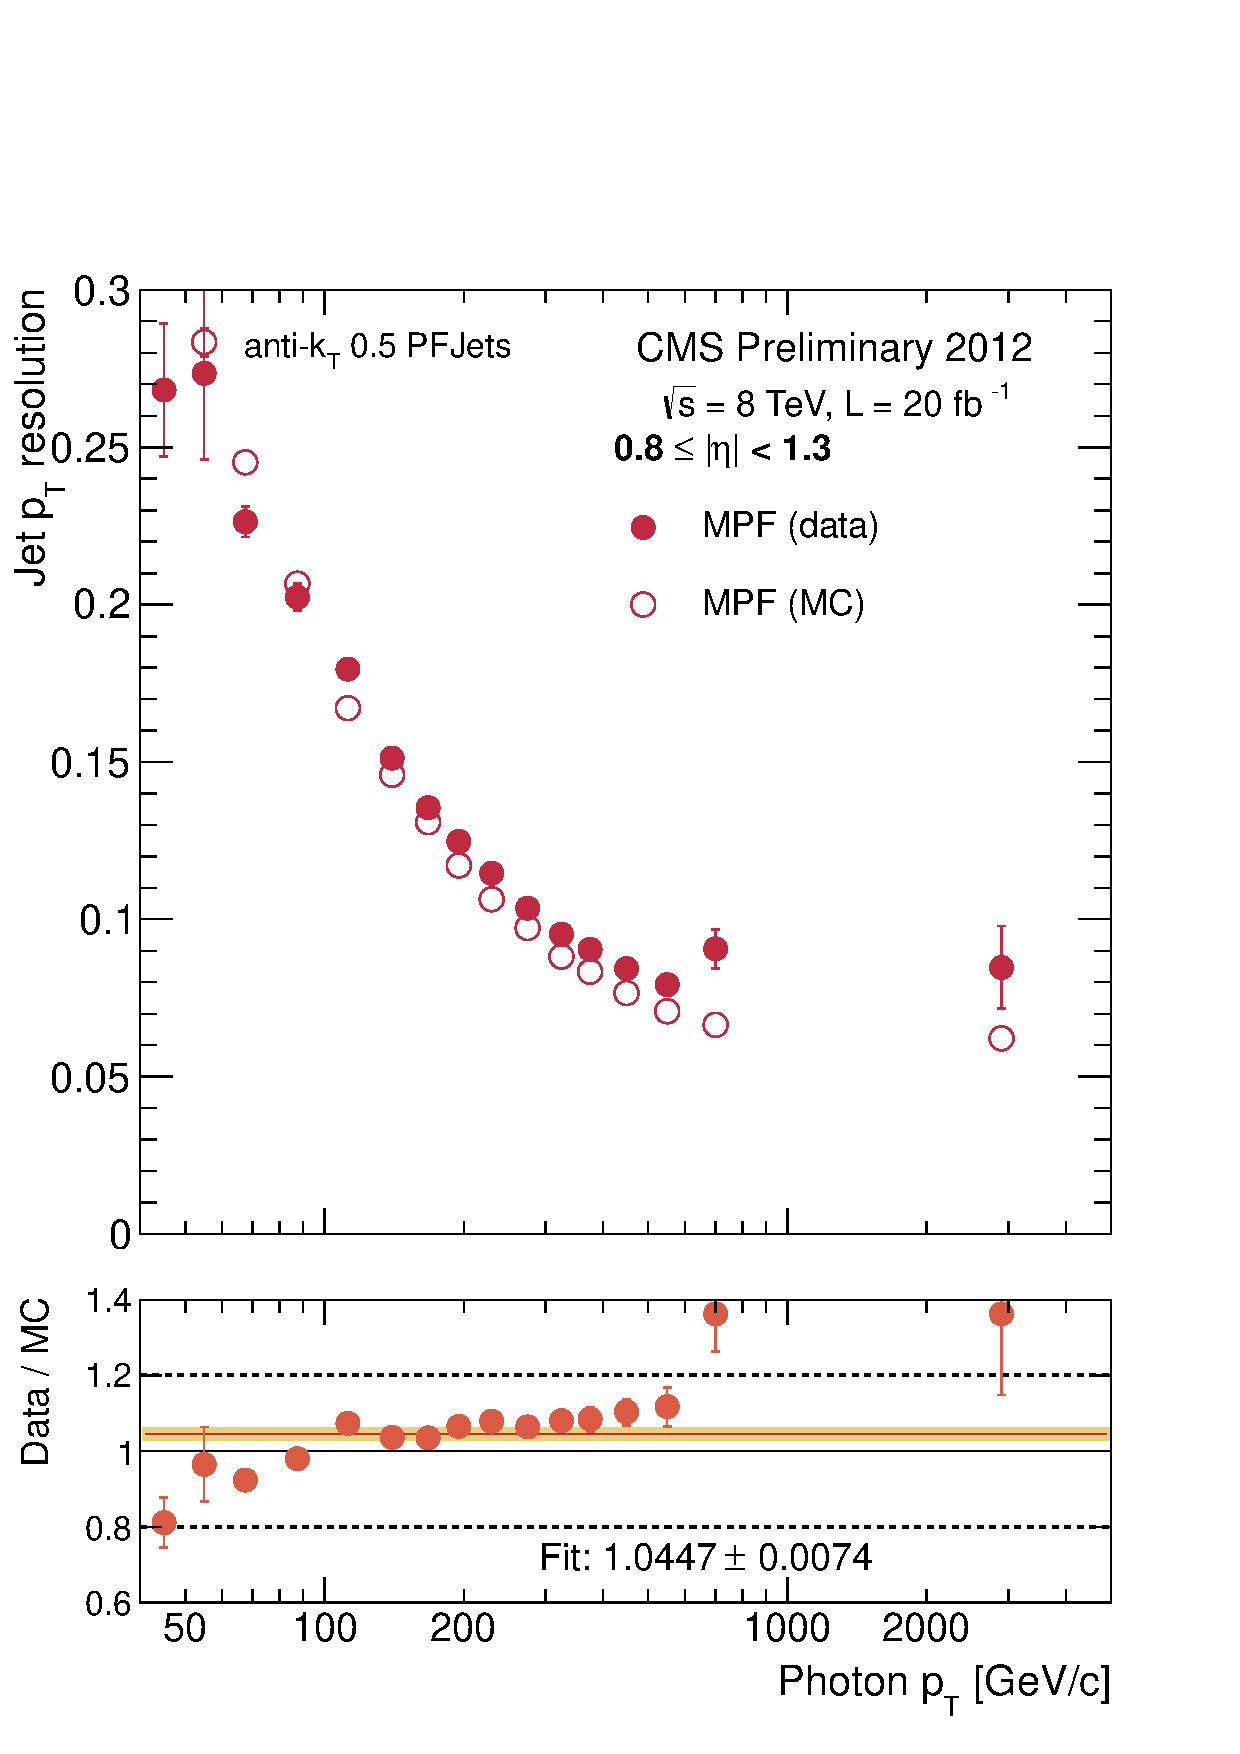
\includegraphics[width=0.45\textwidth]{chapitre4/figs/reso_mpf/resolution_eta0813_mpf.pdf}}
    \subcaptionbox{\label{fig:reso_mpf_eta1319}}[0.45\textwidth]{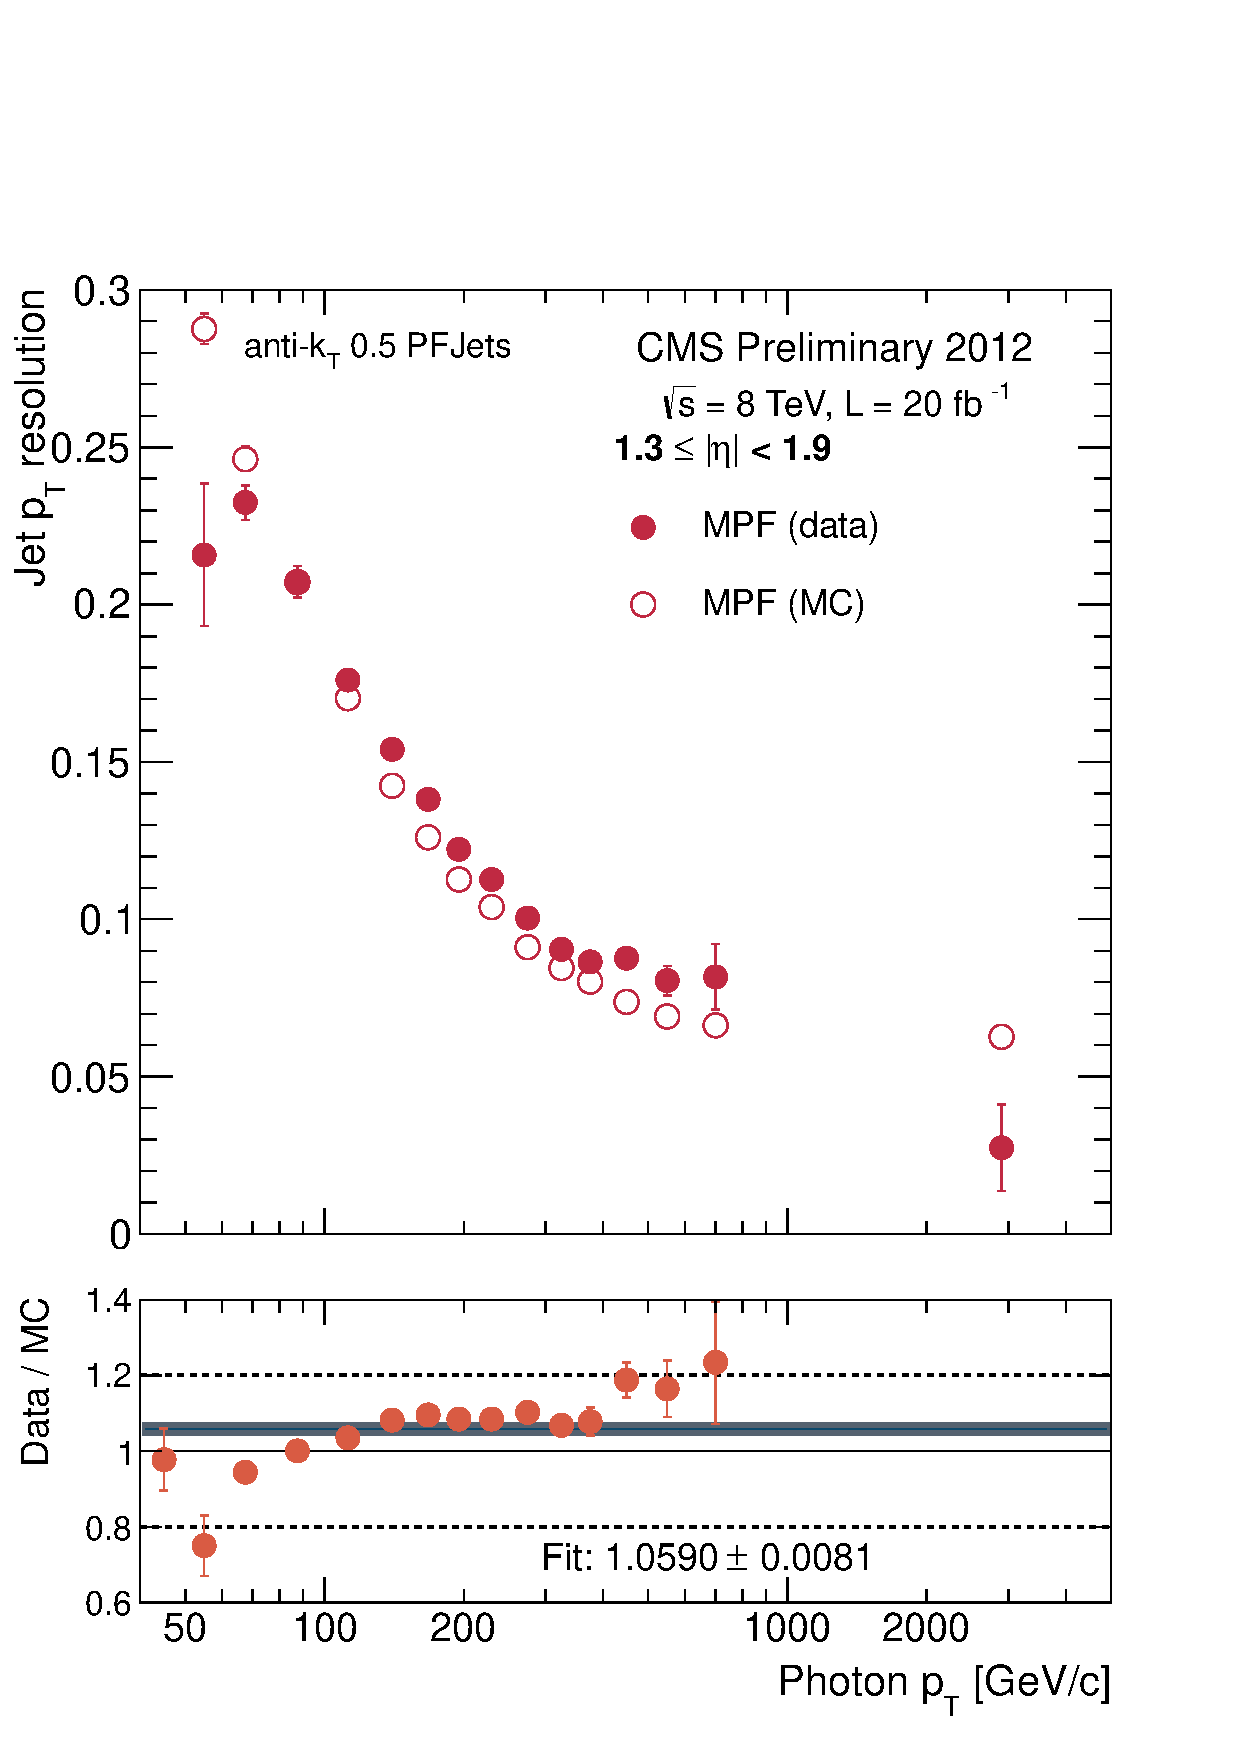
\includegraphics[width=0.45\textwidth]{chapitre4/figs/reso_mpf/resolution_eta1319_mpf.pdf}}\hfill
    \subcaptionbox{\label{fig:reso_mpf_eta1925}}[0.45\textwidth]{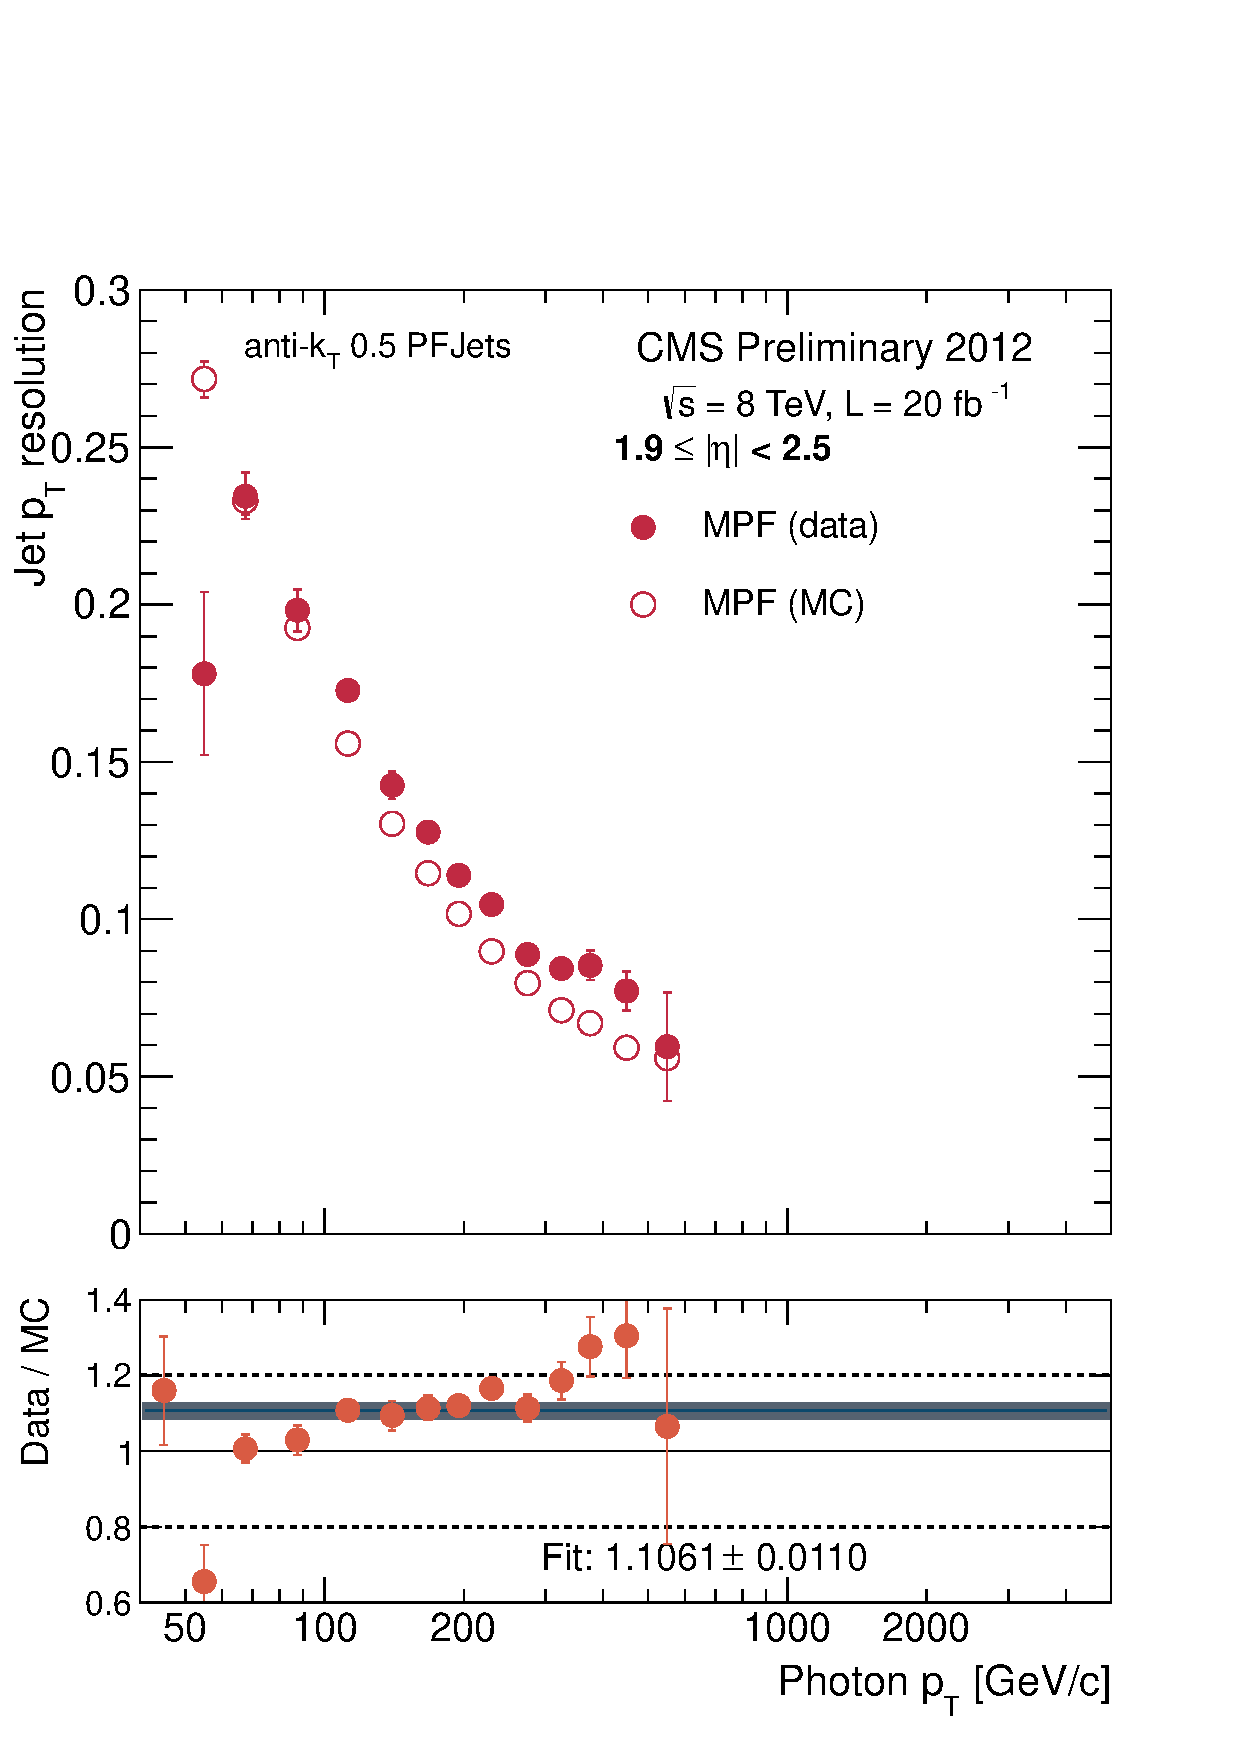
\includegraphics[width=0.45\textwidth]{chapitre4/figs/reso_mpf/resolution_eta1925_mpf.pdf}}
    \caption{Résolutions pour la méthode MPF, sans extrapolation, pour $\aeta < \num{0.8}$ (\subref{fig:reso_mpf_eta008}), $\num{0.8} \leq \aeta < \num{1.3}$ (\subref{fig:reso_mpf_eta0813}), $\num{1.3} \leq \aeta < \num{1.9}$ (\subref{fig:reso_mpf_eta1319}), et $\num{1.9} \leq \aeta < \num{2.5}$ (\subref{fig:reso_mpf_eta1925}). Le ratio entre les données et la simulation est présenté sous chaque distribution, accompagné d'une interpolation linéaire constante (ligne grise)}
    \label{fig:mpf_reso}
\end{figure}

Par rapport à la méthode de la balance, on constate deux améliorations. Premièrement, les ratios sont meilleurs, avec des incertitudes comparables. Deuxièmement, ces ratios sont plus stables en fonction de \aeta, particulièrement à haut \aeta, là où la statistique se réduit.

\begin{figure}[tbp]
    \centering
    \subcaptionbox{\label{fig:npv_bal_eta013}}[0.4\textwidth]{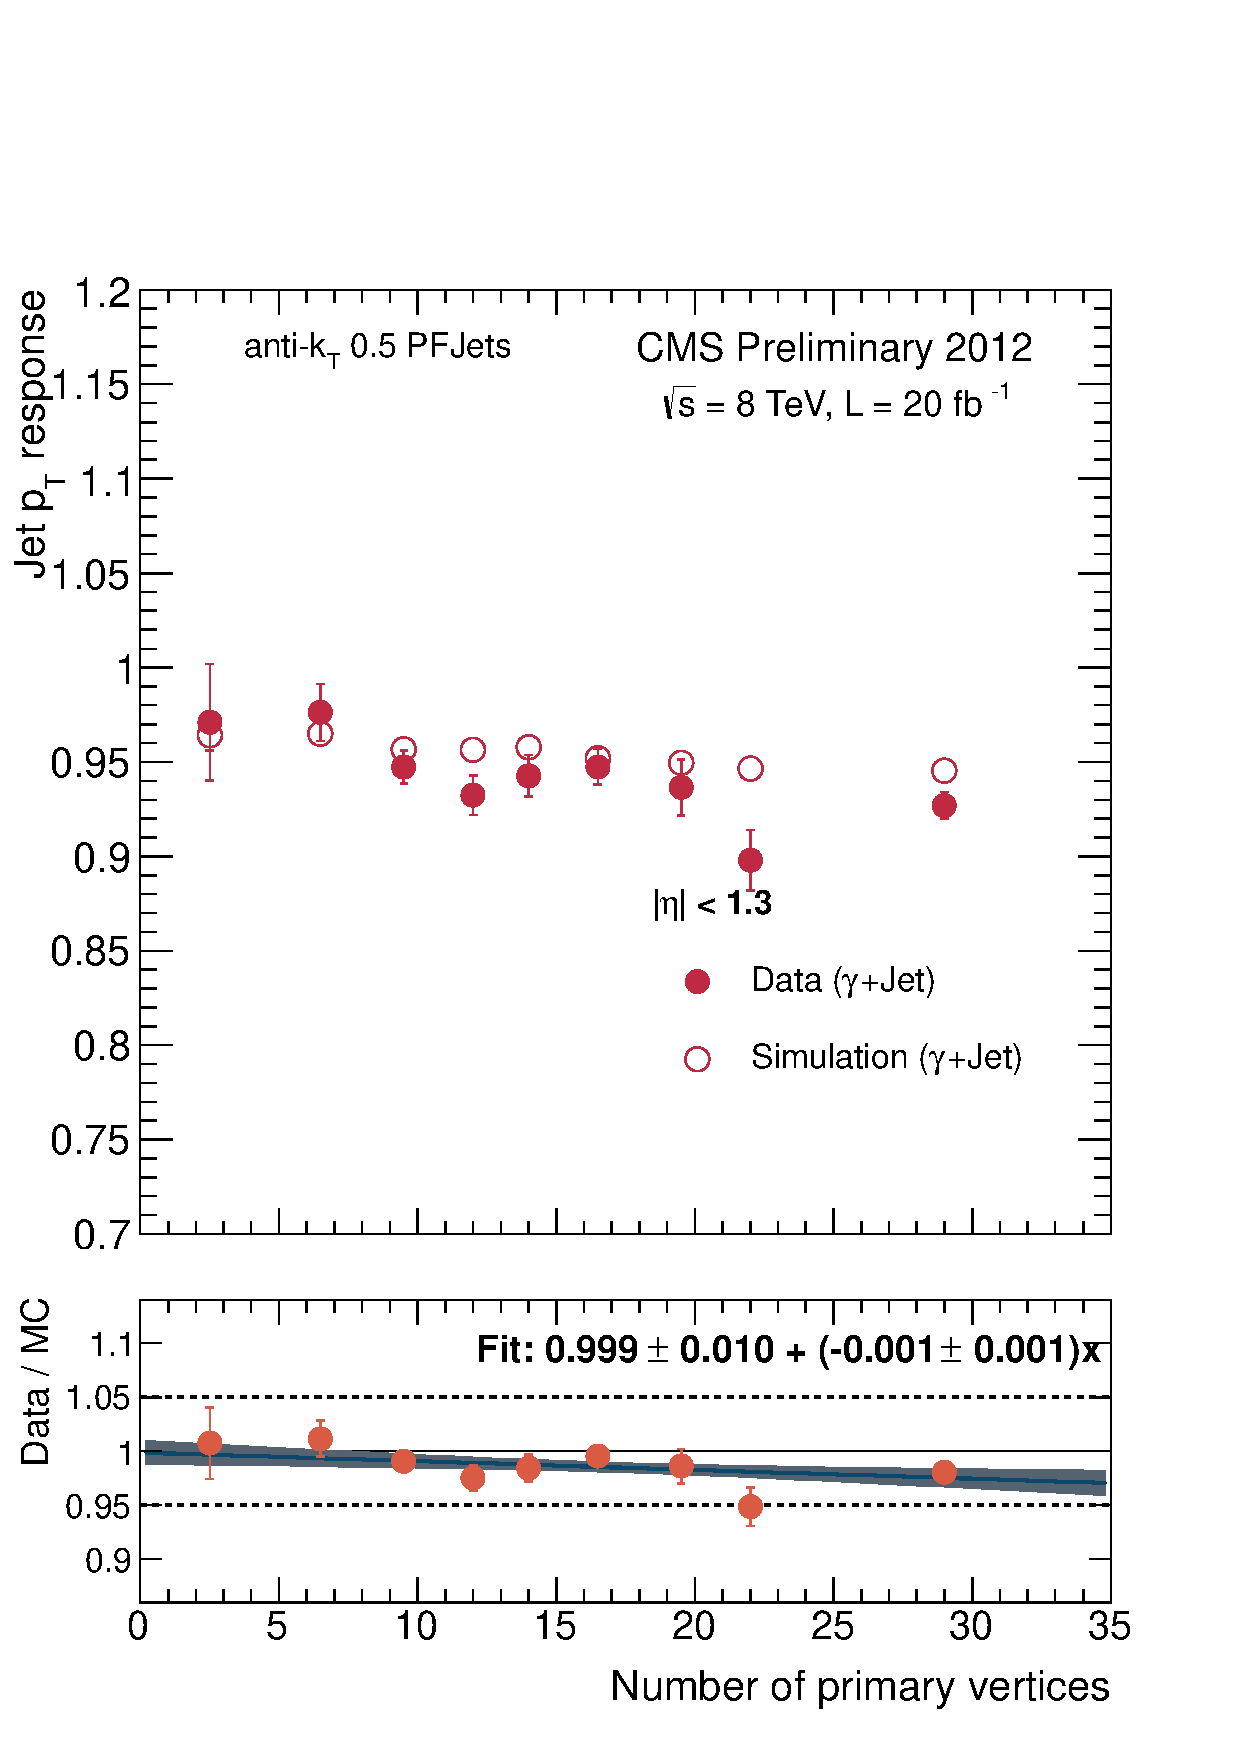
\includegraphics[width=0.4\textwidth]{chapitre4/figs/resp_vs_npv/resp_balancing_eta013_vs_npv_FITLINE.pdf}}\qquad
    \subcaptionbox{\label{fig:npv_mpf_eta013}}[0.4\textwidth]{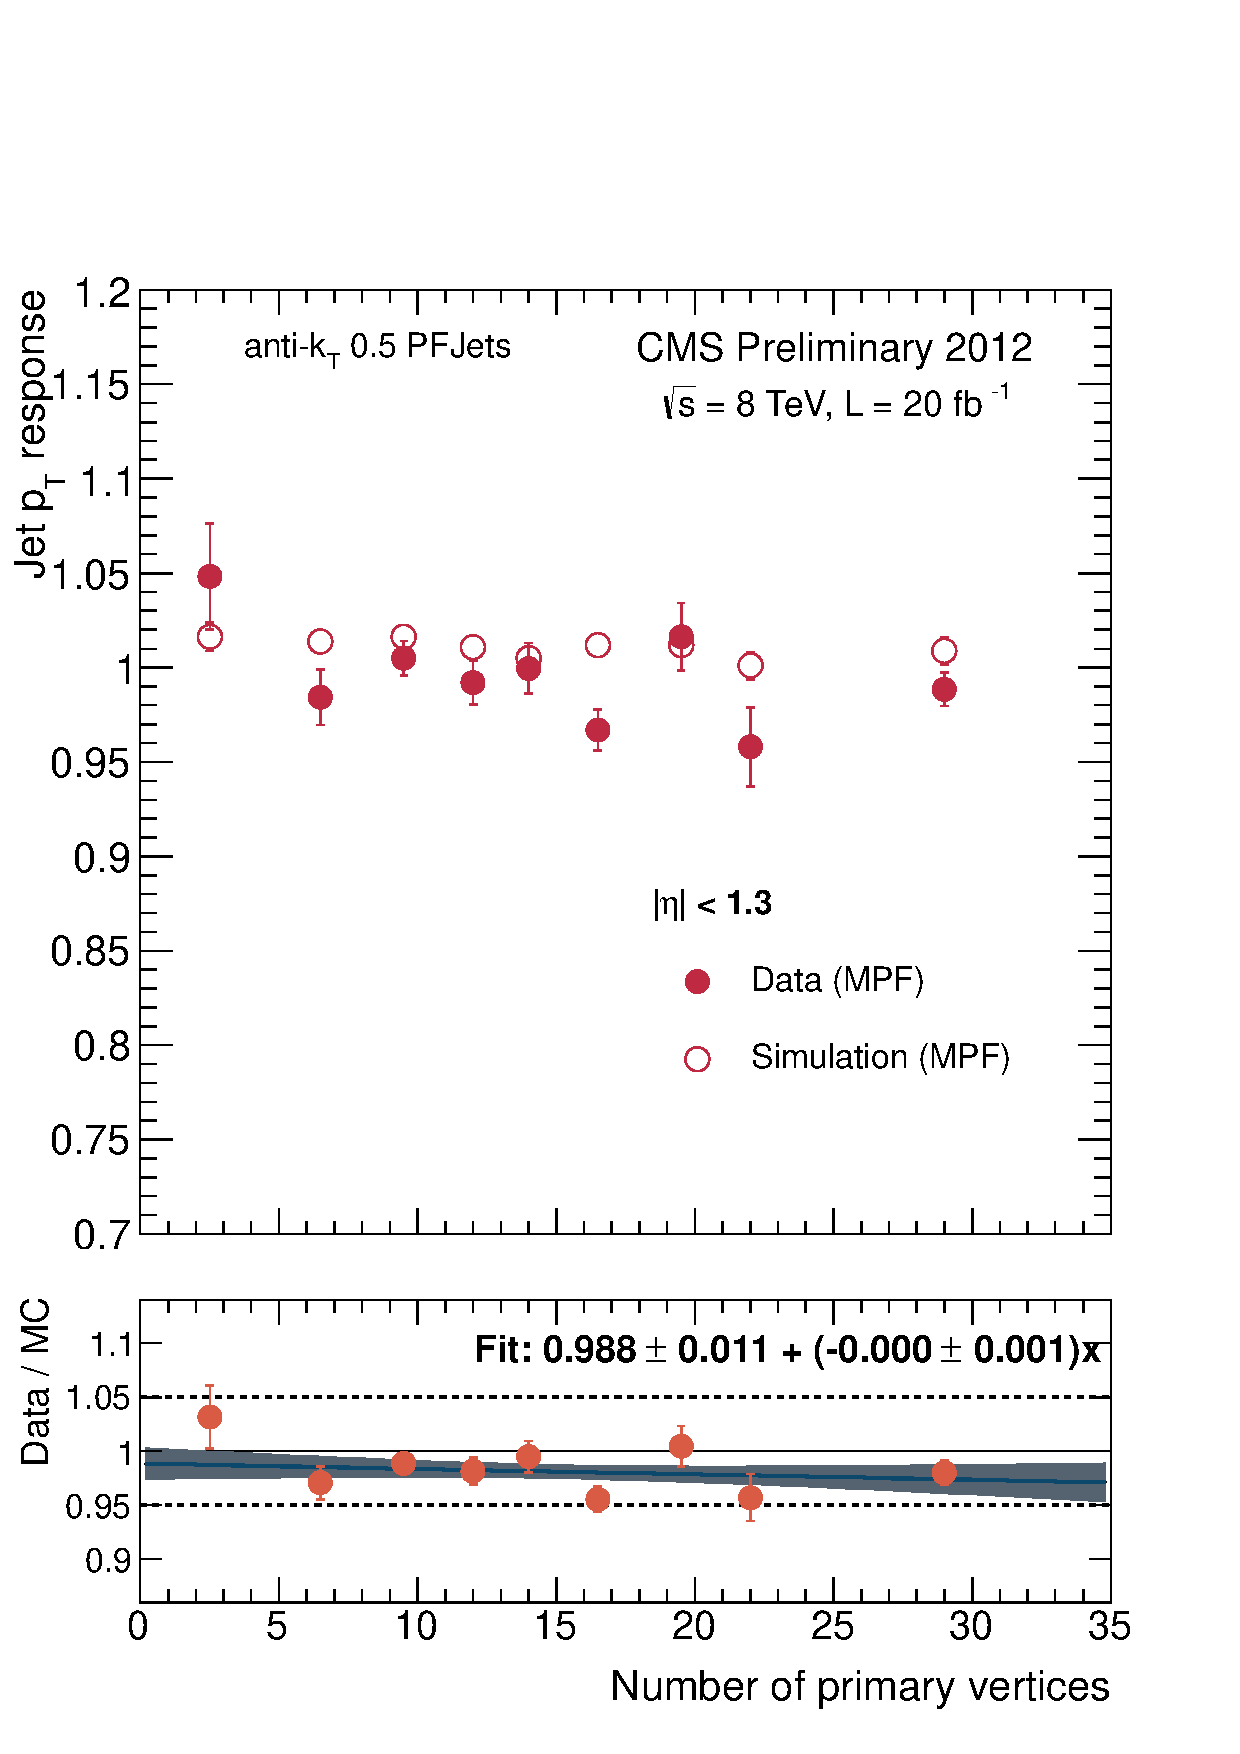
\includegraphics[width=0.4\textwidth]{chapitre4/figs/resp_vs_npv/resp_mpf_eta013_vs_npv_FITLINE.pdf}}
    \caption{Évolution des réponses pour les méthodes de la balance (\subref{fig:npv_bal_eta013}) et MPF (\subref{fig:npv_mpf_eta013}) en fonction du nombre de vertex primaires, variable sensible à la quantité de \pu sans l'événement.}
    \label{fig:resp_vs_npv}
\end{figure}

Au niveau de la résolution, on constate qu'elle est bien meilleure sur les données avec la méthode MPF qu'avec la méthode de la balance. Ce résultat était en effet prévisible, puisqu'on a vu précédemment que la méthode était beaucoup moins sensible à l'activité secondaire dans le détecteur, puisqu'elle utilise dès sa définition la totalité de l'impulsion transverse des particules. Les différences de modélisation du \pu entre données et simulation n'affectent ainsi pas les performances de la méthode MPF. On présente \cref{fig:resp_vs_npv} l'évolution du ratio données sur simulation pour la méthode de la balance et la méthode MPF en fonction du nombre de vertex primaire, variable directement corrélée à la présence de \pu dans la collision. On constate que la réponse de la méthode MPF est plus proche de l'unité, et ce même à haut nombre d'interactions. De plus, le ratio reste stable en fonction du nombre de vertex, contrairement à la méthode de la balance, où on voit une faible évolution.

\subsection{Extraction des corrections résiduelles}

\begin{figure}[tbp]
  \centering
  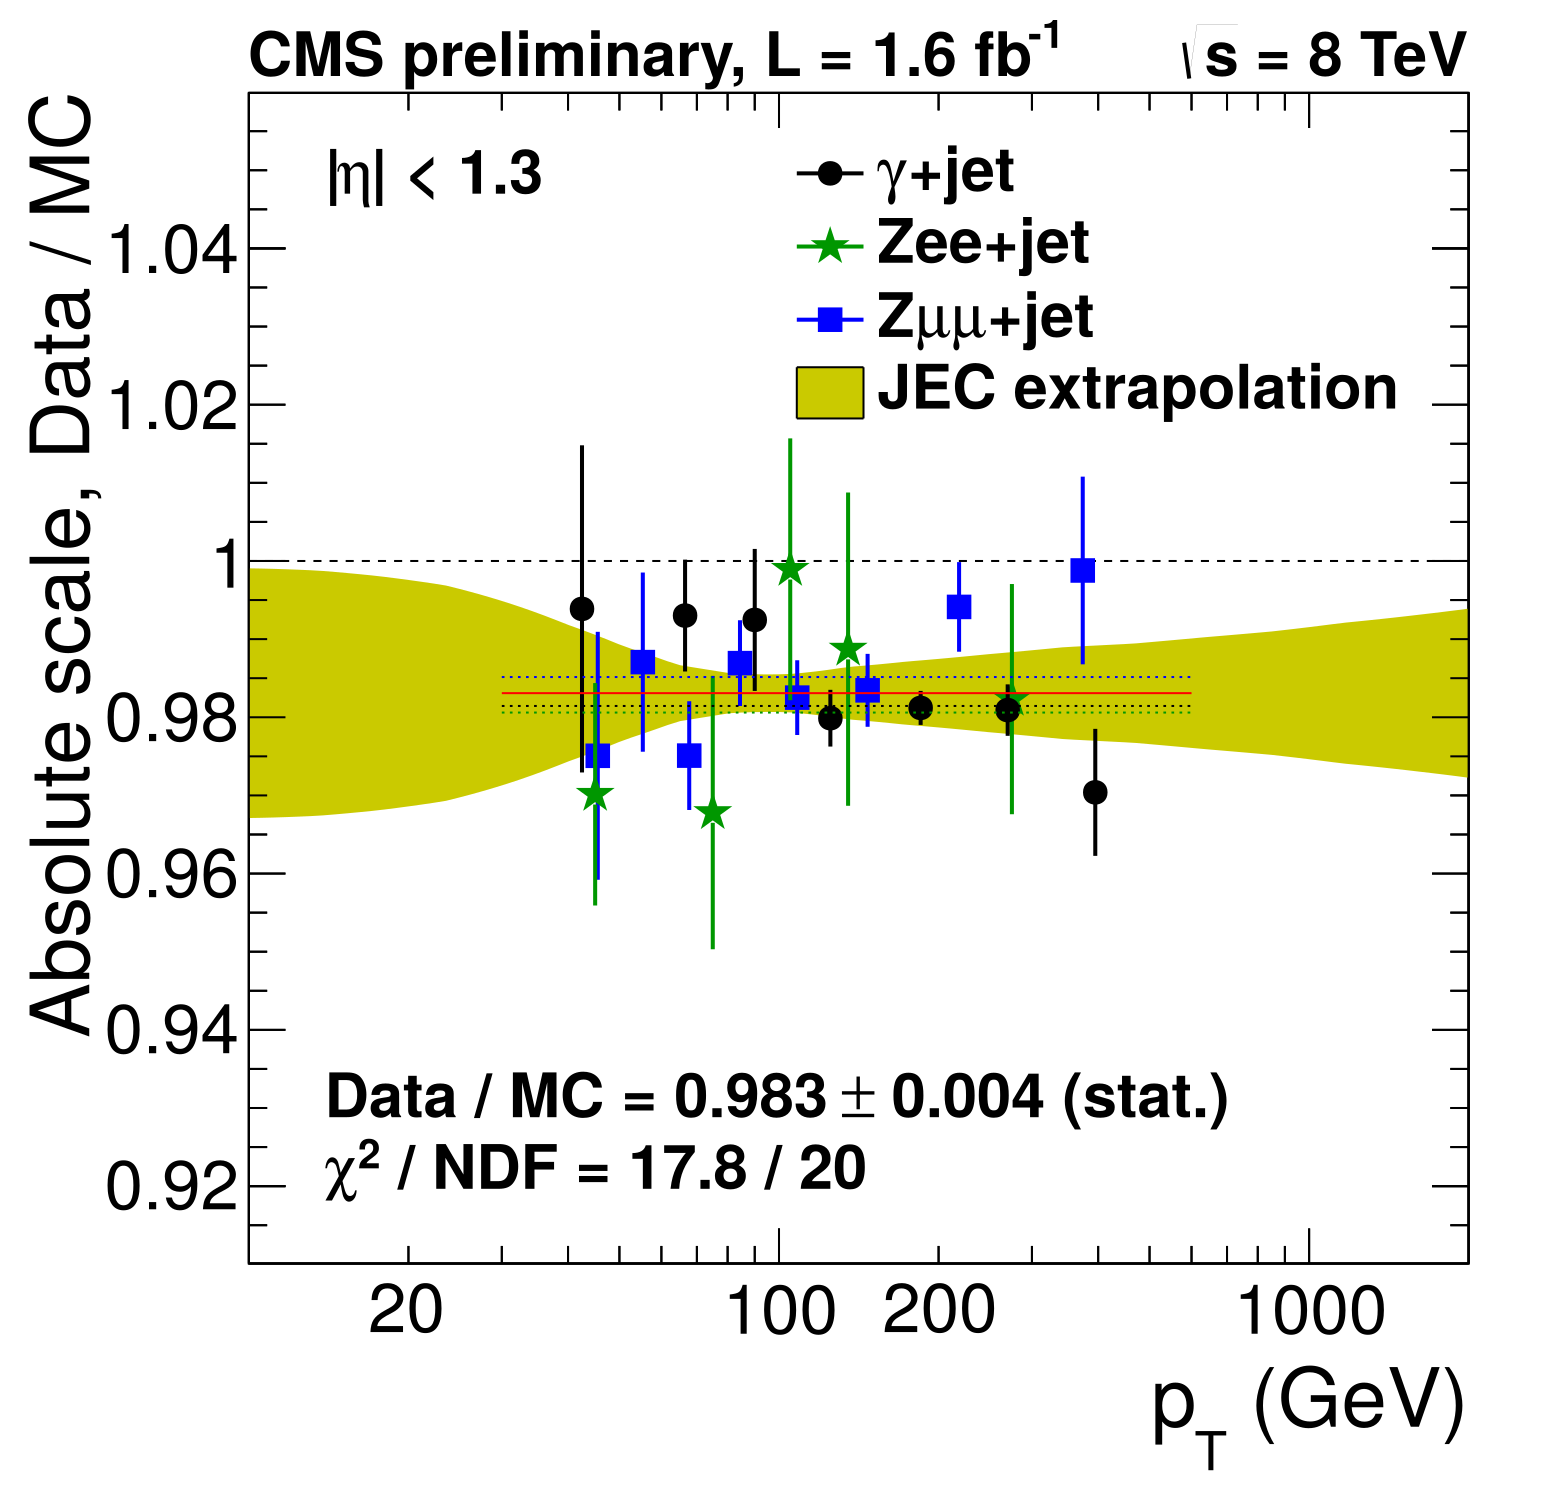
\includegraphics[width=0.5\textwidth]{chapitre4/figs/jec_residuals_combined.pdf}
  \caption{Extraction des facteurs de corrections résiduels grâce à une combinaison entre les analyses $\PZ \rightarrow \Pmuon \APmuon$ + jets, \PZ $\rightarrow$ \Pelectron \APelectron + jets et \Pphoton + jets.}
  \label{fig:jec_residuals_combined}
\end{figure}

Afin d'obtenir les corrections résiduelles finales, on combine les résultats de l'analyse \Pphoton + jets avec les analyses $\PZ \rightarrow \Pmuon \APmuon$ + jets et \PZ $\rightarrow$ \Pelectron \APelectron + jets. L'analyse \PZ $\rightarrow$ \Pelectron \APelectron permet de vérifier directement les résultats obtenus par \Pphoton + jets, puisque ces deux analyses utilisent principalement le calorimètre électromagnétique, et que les objets photons et électrons sont très similaire. L'analyse $\PZ \rightarrow \Pmuon \APmuon$ est plus indépendante des deux autres, et permet de conforter les résultats obtenus avec les autres analyses.

On présente \cref{fig:jec_residuals_combined} la combinaison entre les trois analyses. Une interpolation globale entre les trois résultats permet d'obtenir les facteurs de corrections résiduelles officiels. On constate que tous les résultats sont compatibles entre eux, et on extrait un ratio données sur simulation de \SI{0.983 \pm 0.004}{}. On reproduit la même chose pour chaque classe en \aeta, et on dérive ainsi les corrections résiduelles qui seront utilisés par toute la collaboration.

\subsection{Test d'intégrité (\emph{cross-check})}

\begin{figure}[tbp]
    \centering
    \subcaptionbox{Sans corrections résiduelles\label{fig:mpf_no_residuals_eta013_pt_210_250}}[0.45\textwidth]{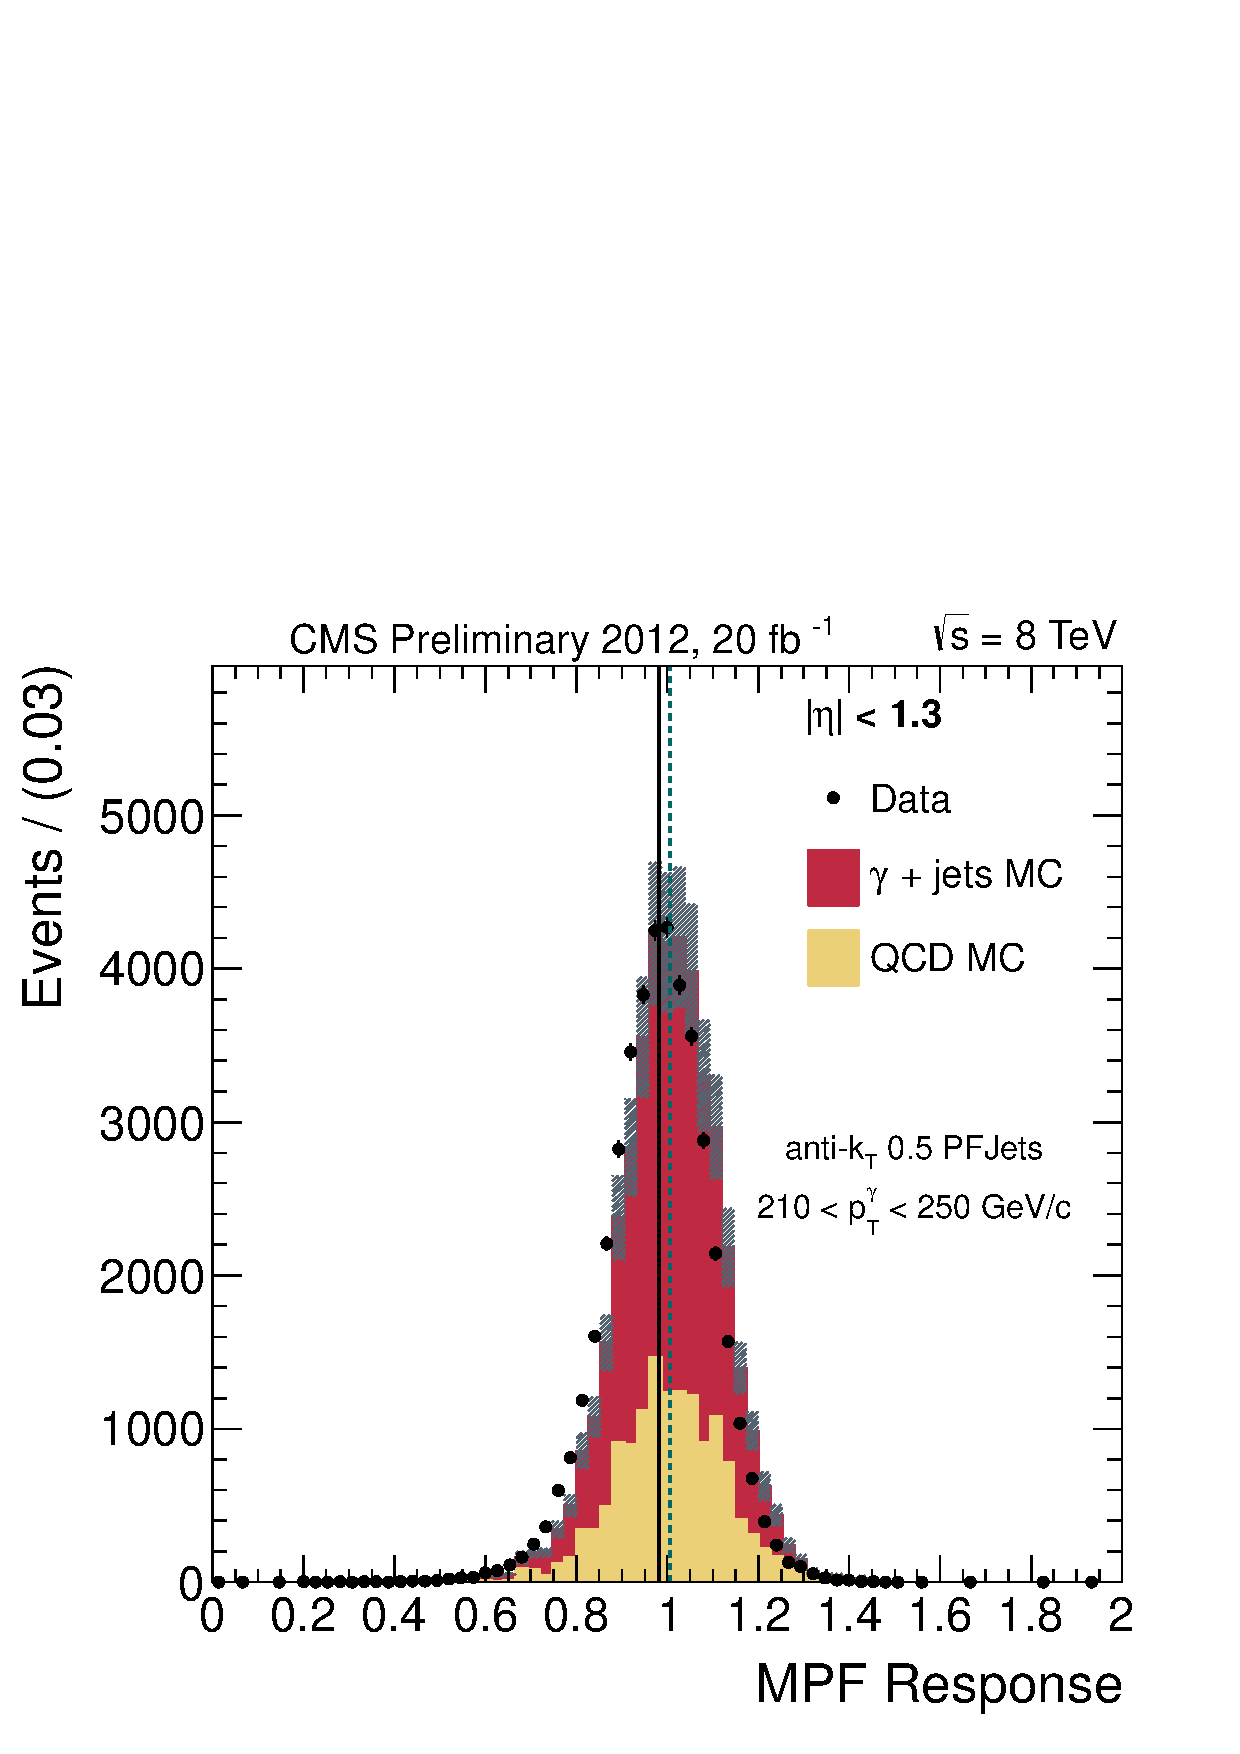
\includegraphics[width=0.45\textwidth]{chapitre4/figs/resp_mpf_eta013_ptPhot_210_250.pdf}} \qquad
    \subcaptionbox{Avec corrections résiduelles\label{fig:mpf_residuals_eta013_pt_210_250}}[0.45\textwidth]{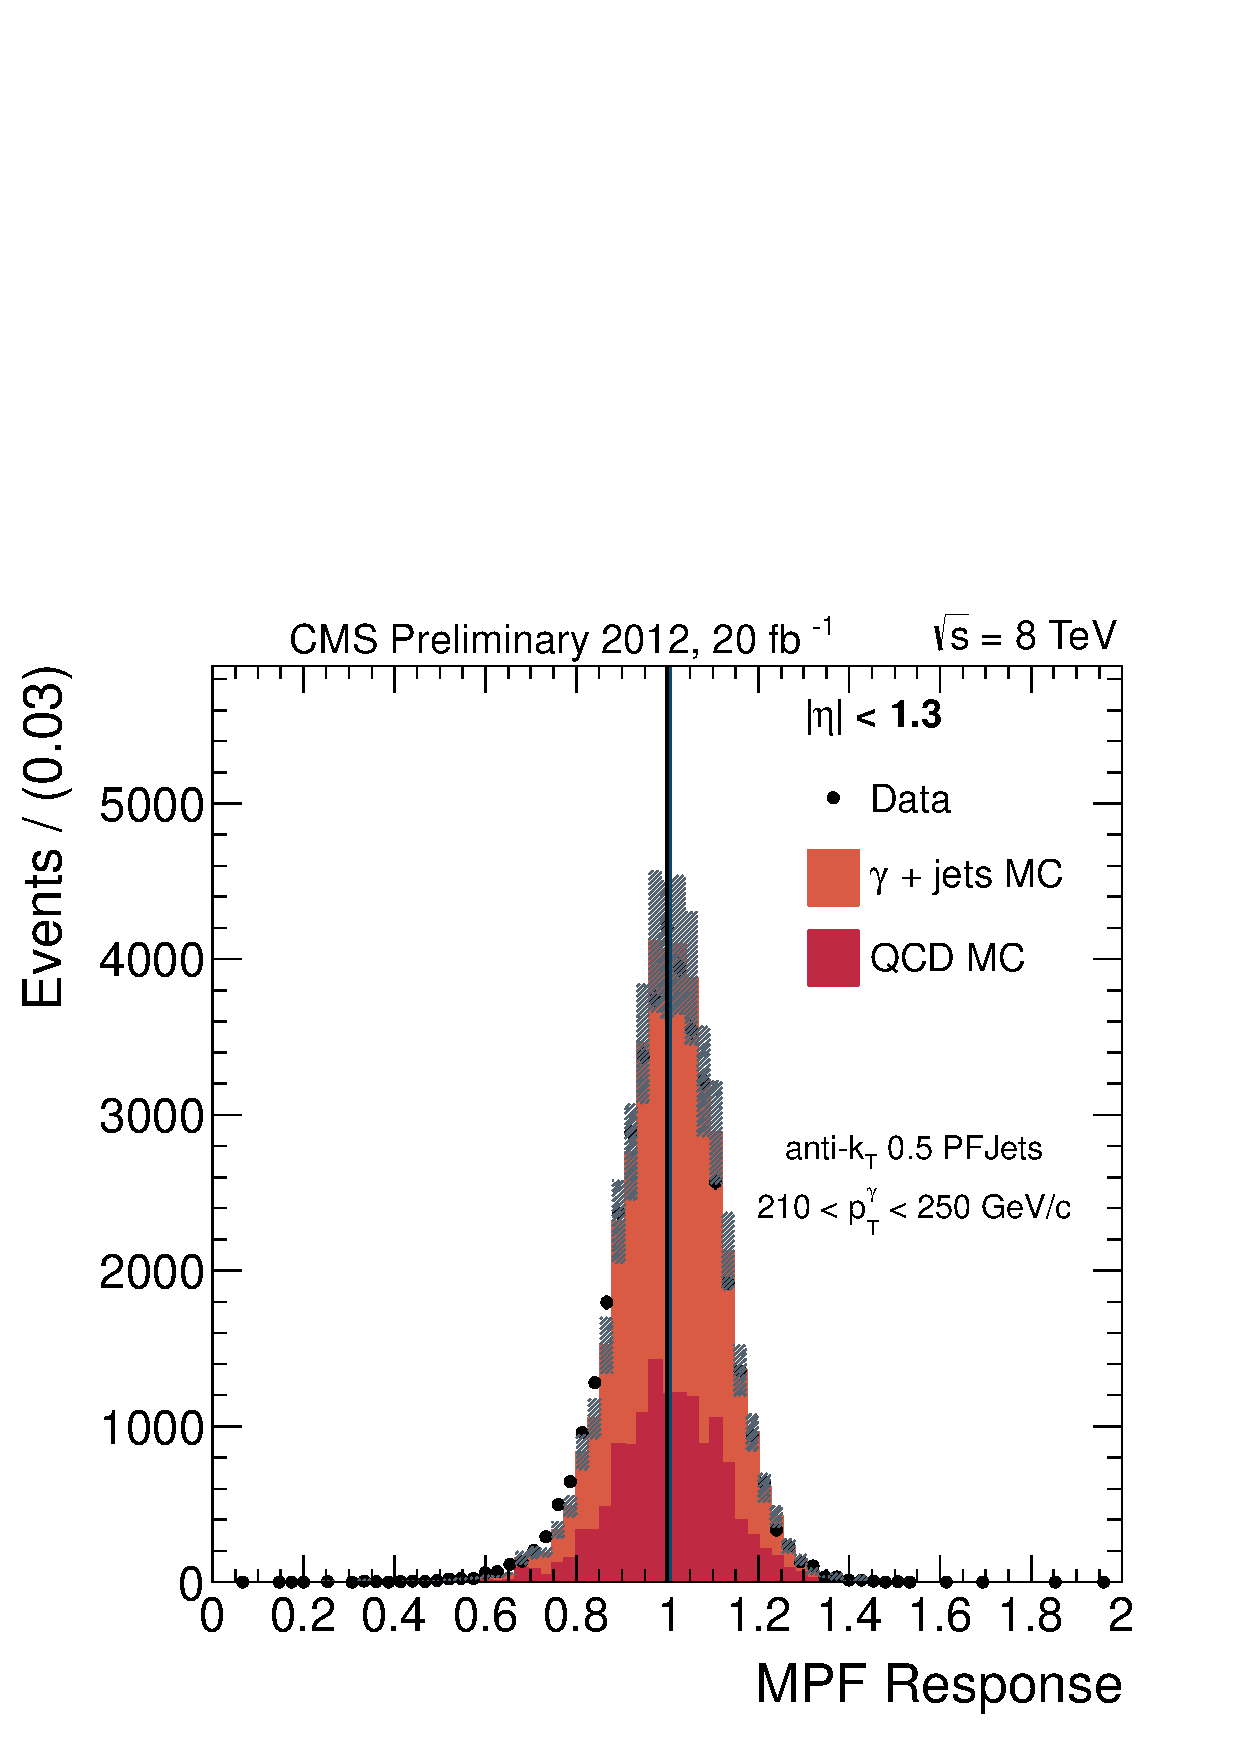
\includegraphics[width=0.45\textwidth]{chapitre4/figs/resp_mpf_eta013_ptPhot_210_250_residuals.pdf}}
    \caption{Réponses pour la méthode MPF pour une en \ptg entre 210 - \SI{250}{\GeV}, pour $\aeta < \num{1.3}$, avec et sans corrections résiduelles.}
    \label{fig:comp_mpf_residuals}
\end{figure}

Les corrections résiduelles déterminées, on peut maintenant vérifier l'effet produit. Pour cela, on recommence l'analyse en corrigeant les jets avec tous les niveaux de corrections disponibles, et on extrait les nouveaux ratios des réponses. Si tout est parfait, on s'attend à obtenir des ratios proche de 1.

On présente \cref{fig:comp_mpf_residuals} la distribution des réponses pour une classe en \ptg entre 210 - \SI{250}{\GeV} pour la méthode MPF, sans corrections résiduelles (\subref{fig:mpf_no_residuals_eta013_pt_210_250}) et avec (\subref{fig:mpf_residuals_eta013_pt_210_250}). On constate bien une amélioration de la réponse moyenne sur les données grâce à l'ajour des corrections résiduelles : le décalage observé précédemment entre les distributions des réponses données et simulation a disparu. Afin de confirmer cette observation, on peut voir \cref{fig:comp_mpf_residuals_2} les distributions des réponses moyennes après application des corrections résiduelles. Comme prévu, le ratio est amélioré par rapport au \cref{tab:res_mpf}. Néanmoins, le ratio n'est pas égal à 1, même avec les incertitudes. En effet, les corrections résiduelles sont extraites en combinant 3 analyses différentes, ce qui explique qu'on ne retrouve pas un ratio de 1, comme cela aurait été le cas si les corrections étaient dérivées uniquement avec l'analyse \Pphoton + jets. Les corrections sont donc validées.

\begin{figure}[tbp]
    \centering
    \subcaptionbox{\label{fig:resp_mpf_residuals_eta008}}[0.45\textwidth]{\includegraphics[width=0.45\textwidth]{chapitre4/figs/resp_mpf_residuals/response_eta008_mpf.pdf}} \qquad
    \subcaptionbox{\label{fig:resp_mpf_residuals_eta0813}}[0.45\textwidth]{\includegraphics[width=0.45\textwidth]{chapitre4/figs/resp_mpf_residuals/response_eta0813_mpf.pdf}}
    \caption{Réponses moyennes pour la méthode MPF, après corrections résiduelles, pour deux classes \aeta : $\num{< 0.8}$ et \num{0.8} - \num{1.3}.}
    \label{fig:comp_mpf_residuals_2}
\end{figure}

\section{Conclusion}

Au travers de ce chapitre, on a vu en détails comment CMS corrige l'énergie des jets. L'enjeu est en effet important, puisqu'une mauvaise calibration des jets peut avoir d'énormes conséquences. Ainsi, l'expérience CDF du Tevatron publie en 2011 un nouveau résultat et annonce la mise en évidence d'une nouvelle résonance dans le spectre de masse di-jet, à environ \SI{125}{\GeV} \citep{CDF_old}. Cependant, l'expérience partenaire au Tevatron, D0, ne voit elle aucun signe de cette résonance dans ces propres données. Il s'avère qu'il s'agissait en réalité d'un problème de corrections en énergie des jets entre les jets de gluons et les jets de quarks, confirmé il y a peu \citep{CDF_new}. Il est donc capital de maitriser le mieux possible ces corrections en jets.

\bigskip

Les événements \Pphoton + jets sont de puissants outils pour déterminer les facteurs de corrections résiduelles des jets. On utilise en effet l'excellente reconstruction des photons pour contraindre l'énergie des jets. On obtient ainsi des facteurs de corrections, utilisés globalement par toute la collaboration CMS. On verra d'ailleurs dans les prochains chapitres que ces corrections sont utilisés dans nos autres analyses afin de corriger efficacement nos jets.

\bigskip

D'autres travaux sont actuellement en cours dans CMS pour la correction des jets. Ainsi, des études sont menées pour déterminer des facteurs de corrections dépendants de la saveur des jets (jet de \Pbottom, jet de gluon, \ldots), et des améliorations sont aussi attendus au niveau des corrections de niveau 1 afin de réduire encore plus la dépendance en fonction du nombre de \pu.